% !TeX encoding = UTF-8
% !TeX program = pdflatex
% IEEEtran Journal Template -- Migrated from Elsevier cja-template.tex
\documentclass[lettersize,journal]{IEEEtran}

%% ---- Packages (only those compatible with IEEEtran) ----
\usepackage{amsmath,amsfonts,amssymb}
\usepackage{algorithm}
\usepackage{algorithmic}    % IEEEtran recommends algorithmic (not algorithmicx)
\usepackage{array}
\usepackage{bm}
\usepackage{booktabs}
\usepackage{multirow}
\usepackage{graphicx}
\usepackage{url}
\usepackage{cite}           % IEEE-style numeric citations
\usepackage{textcomp}
\usepackage{stfloats}       % allows figure* at bottom
\usepackage{placeins}       % keep each case's figures within its subsection
% \usepackage[caption=false,font=normalsize,labelfont=sf,textfont=sf]{subfig}
\usepackage[caption=false,font=footnotesize,labelfont=sf,textfont=sf]{subfig}
\usepackage{siunitx}

% ---- Clean submission version: revision markup removed ----
% Graphics used by the revised manuscript are consolidated in all_fig
\graphicspath{{all_fig/}}
% 3D (V10) result figures for the revised simulation section
\newcommand{\vfig}[1]{all_fig/#1}
% Updated PN results for the two maneuvering-target cases
\newcommand{\pncasefig}[1]{all_fig/#1}

% theorem/lemma environments
\newtheorem{theorem}{Theorem}
\newtheorem{lemma}{Lemma}

\hyphenation{op-tical net-works semi-conduc-tor IEEE-Xplore}

% ----------------------------------------------------------------
\begin{document}

% ---- Title ----
% \title{Multi-Agent Reinforcement Learning-Based Cooperative Interception Strategy
%   for Maneuvering Swarm Attack Targets with Considering Target Assignment}

% \title{Trust-Aware Multi-Agent Reinforcement Learning-Based Cooperative Interception Strategy for Maneuvering Swarm Attack Targets Considering Rapid Consensus Target Assignment}
\title{Trust-Aware Multi-Agent Reinforcement Learning-Based Cooperative Interception Strategy for Maneuvering Swarms with Target Assignment}

% ---- Authors ----
% \author{Shuyi~Gao,~Defu~Lin,~Duo~Zheng,~and~Zhichen~Chu%
% \thanks{S. Gao, D. Lin, D. Zheng, and Z. Chu are with the School of Aerospace
% Engineering, Beijing Institute of Technology, Beijing 100081, China
% (e-mail: zhengduohello@126.com).}%
% \thanks{Manuscript received 2025.}}

%----双盲投稿--
\author{}
\markboth{Under review}%
{Anonymous Submission}

% ---- Running heads ----
\markboth{IEEE Transactions on Automation Science and Engineering}%
{Gao \MakeLowercase{\textit{et al.}}: MARL-Based Cooperative Interception for Maneuvering Swarm Targets}

\maketitle

% ---- Abstract ----
\begin{abstract}
The swarm attack of unmanned aerial vehicles (UAVs) poses a significant threat to future
battlefield operations.
Achieving efficient and precise cooperative interception against attacking UAV swarms with
highly dynamic maneuvering capabilities and adaptive penetration strategies poses a critical
challenge for UAV interceptor swarms.
This study addresses the cooperative interception of maneuvering targets in swarm attacks by
decomposing the problem into two key tasks: target assignment and cooperative interception
guidance.
For target assignment, an Improved Dung Beetle Optimization (IDBO) algorithm is proposed to
dynamically balance exploration and exploitation, achieving highly efficient and rapid
assignments.
% For cooperative interception guidance, a multi-agent deep reinforcement learning-based method
% is developed to achieve precise and time-coordinated interception of adversarial UAV swarms
% employing advanced penetration strategies.
% For cooperative interception guidance, a multi-agent deep reinforcement learning framework—augmented by kinematics-aware attention mechanisms and trust-modulated exploration—is developed to achieve precise and time-coordinated interception of adversarial UAV swarms employing advanced penetration strategies.
For cooperative interception guidance, an Attention-Residual and Trust-aware Multi-Agent Proximal Policy Optimization (ART-MAPPO) framework is developed to achieve precise and time-coordinated interception of adversarial UAV swarms employing advanced penetration strategies.
The simulation results validate the effectiveness of the proposed intelligent cooperative
interception method, demonstrating superior convergence speed, robustness, and significantly
improved interception success rates in swarm UAV cooperative interception scenarios.
\end{abstract}

{\linespread{0.9}\selectfont
\hspace*{0.0em}\textbf{\textit{Note to Practitioners—}}\textbf{This paper is motivated by practical UAV swarm defense scenarios, where multiple interceptors must cooperatively engage maneuvering aerial targets under limited communication and onboard maneuver constraints. In such applications, target assignment and guidance are closely coupled, and conventional centralized approaches may be difficult to implement efficiently as the engagement scale increases. To address this issue, this paper develops a two-stage cooperative interception framework that combines distributed target assignment with a trust-aware multi-agent reinforcement learning guidance method. The proposed approach is intended to improve coordination consistency among interceptors assigned to the same target and to enhance robustness against target maneuvers while considering maneuver saturation and command smoothness. This work may be useful for practical large-scale multi-UAV interception and other cooperative autonomous systems requiring scalable distributed decision-making and coordinated guidance.}\par\vspace{0.5\baselineskip}
}

% ---- Keywords ----
\begin{IEEEkeywords}
Cooperative interception, deep reinforcement learning, centralized training with decentralized
execution, target assignment, UAV swarm.
\end{IEEEkeywords}


%% ===========================================================
\section{Introduction}
\label{sec:introduction}
\IEEEPARstart{A}{s} warfare evolves toward intelligent swarm operations, the likelihood of
encountering attacks from adversarial UAV swarms significantly increases during combat.
Consequently, the efficient interception of incoming swarm targets becomes a critical
imperative for future battlefield operations.
To address the challenge of cooperative interception against maneuvering attacking swarms with
adaptive penetration strategies, there is an urgent need to advance academic research in swarm
target interception technologies.
This study aims to enhance interceptors with intelligent cooperative interception capabilities,
enabling effective navigation of complex challenges in modern battlefield environments.

Multi-target cooperative interception encompasses two key tasks: target assignment and
cooperative interception.
The effectiveness of multi-target interception hinges on the optimality of target assignment,
establishing it as a primary focus in swarm target interception strategies.
As the number of UAVs increases, the complexity of target assignment escalates significantly,
resulting in a multi-constrained, multi-parameter optimization problem.
The objective is to develop a rapid and efficient target assignment method for allocating
specific attacking targets to interceptors in operational scenarios~\cite{KLINE2019226}.
The target assignment problem involves complex constraints, and the non-dominated sorting
algorithm can dynamically generate a set of reference points with good convergence and
distribution performance~\cite{WANG2025952,bai2024hybrid,zou2024moea}.
Moreover, employing an online operator selection mechanism can enhance the efficiency of the
algorithm~\cite{ahmad2024fuzzy,ming2024constrained}.
The target assignment problem can be solved using multi-information particle swarm optimization
to find the solution that yields the highest gain~\cite{mishra2015weapon,wei2020particle}.
Introducing information from surrounding particles can enhance the stability of the traditional
particle swarm algorithm while also addressing the issue of local convergence in the target
assignment problem~\cite{long2024improved}.
The genetic algorithm is a common approach for solving the target assignment
problem~\cite{he4914655modelling,li2020multi,sun2022multi,chang2018solving}, and a GA with a
novel crossover operator can further enhance algorithmic efficiency~\cite{weng2024diversity}.
Ant colony optimization is also an effective strategy for solving the target assignment
problem~\cite{li2024comprehensive}, and its combination with a greedy algorithm can improve
the accuracy of parallel computation~\cite{yi2024solving}.
Under multiple constraints, researchers have proposed various heuristic algorithms to solve the
target assignment problem, such as neural networks~\cite{li2024comprehensive}, auction
algorithm~\cite{wang2024collaborative}, tabu search~\cite{yao2024tabu}, simulated annealing
algorithm~\cite{khurshid2024hybrid}, VLSN~\cite{yue2024graph}.
Recent studies have further addressed distributed task allocation
and safe coordination in networked robot teams
~\cite{miele2025distributed}, dynamic multi-UAV assignment under weak
communication~\cite{yu2025dynamic}, and real-time task allocation for UAV
swarms in complex environments~\cite{wang2026realtime}.
However, in cooperative interception scenarios, the aforementioned algorithms struggle to
handle the highly dynamic nature of the battlefield due to their high time complexity, and they
fail to meet the dual requirements of both speed and optimality.

The effectiveness of the terminal guidance phase in multi-target interception is significantly
influenced by the cooperative guidance law, a critical factor requiring thorough consideration.
The target assignment strategy transforms swarm operations into a coordinated multi-to-one
interception problem, with current research focusing on three key areas: angular coordination,
temporal coordination, and intelligent cooperation.
Significant progress has been made in temporal coordination.
Classical proportional navigation-based guidance laws enable synchronized multi-missile attacks
on a single target~\cite{tao2024analytical}.
Adaptive control methods adjust attack timing based on real-time operational conditions, making
them suitable for intercepting maneuvering targets~\cite{wang2025generalized,zhang2022multiple}.
Sliding Mode Control (SMC) is widely adopted for cooperative
interception~\cite{sinha2020supertwisting}, with SMC incorporating miss distance and attack
time constraints enhancing interception
accuracy~\cite{shen2025three,jin2025cooperative,hu2019sliding}.
Considerable research has also been conducted on angular coordination.
From a traditional control perspective, backstepping control~\cite{li2024adaptive} and
leader-follower cooperative methods~\cite{he2017impact} significantly improve interception
efficiency.
SMC with angular constraints is prevalent in cooperative interception, encompassing approaches
based on impact angle constraints~\cite{wang2025hybrid} and line-of-sight angle
constraints~\cite{li2024near}.
Optimal control methods applied to impact angle-constrained cooperative guidance enhance
precision by integrating impact angle and line-of-sight angle
constraints~\cite{wang2025adaptive,tao2023optimal}.

Recent advancements in intelligent technologies have driven extensive research into cooperative
interception strategies for UAV swarms, with intelligent algorithms demonstrating substantial
potential in addressing complex multi-target scenarios~\cite{chen2024enhanced,wu2020collaborative}.
Optimization-based approaches, such as Particle Swarm Optimization (PSO), excel in
collaborative attack problems by autonomously optimizing resource allocation and maximizing
operational efficiency~\cite{zhao2024hierarchical,wu2020collaborative}.
Search-based algorithms, like A*~\cite{liao2024research}, enable efficient path planning for
coordinated attacks.
Control-based methods, including Model Predictive Control
(MPC)~\cite{kim2024adaptive}, provide robust guidance under dynamic constraints.
Moreover, the integration of neural networks with reinforcement learning, particularly deep
reinforcement learning (DRL), enhances the adaptability and intelligence of interception
strategies~\cite{luo2022uav,zhan2022multiple,wang2021uav}.
DRL enables UAV swarms to learn complex policies from high-dimensional data, optimizing target
assignment and maneuvering in real-time to counter maneuvering targets~\cite{sun2024memory}.
Recent studies have further investigated attention-based
reinforcement learning for adaptive UAV-swarm flocking
~\cite{mu2026attention} and reinforcement-learning-based multi-agent path
planning with formation containment~\cite{li2026path}.
In contrast, conventional cooperative interception guidance methods rely heavily on
linearization and simplifying assumptions to design feasible guidance laws~\cite{zhao2025global}.
These methods often struggle to address the complexity of dynamic, non-linear environments
involving maneuvering swarm targets.
Data-driven intelligent cooperative interception methods, by contrast, leverage extensive
datasets to learn adaptive strategies, significantly reducing dependence on restrictive
assumptions~\cite{fainkich2025cooperative}.
By modeling complex interactions through neural networks and DRL, these methods achieve greater
robustness and flexibility.
Despite advancements, intelligent cooperative interception methods struggle with maneuvering
swarm targets in complex dynamic environments due to limited model generalization, low training
efficiency, and low interception success rates, particularly in large-scale swarm combat
requiring precise temporal coordination~\cite{horyna2023decentralized}.
Addressing these challenges requires further research into scalable, generalizable, and
efficient algorithms to fully realize the potential of intelligent cooperative interception.

In summary, existing cooperative interception methods for countering attacking UAV swarms with
adaptive penetration capabilities suffer from low interception success rates in complex dynamic
environments.
Specifically, target assignment methods exhibit low allocation efficiency, while cooperative
interception guidance strategies struggle with terminal acceleration saturation and insufficient
adaptability to dynamic target maneuvers in practical scenarios, hindering effective swarm
coordination.
Consequently, more research is necessary to address these challenges.

This study proposes a swarm cooperative interception method based on multi-agent reinforcement
learning and IDBO algorithm, enhancing target assignment efficiency and guidance strategy
performance to achieve precise and efficient interception of maneuvering targets.
The proposed intelligent cooperative interception algorithm offers the following advantages.

\begin{enumerate}
\item A distributed consensus-based target assignment scheme is proposed, which integrates an
improved Dung Beetle Optimization (IDBO) algorithm with a combat-dominance assessment model.
This design supports rapid many-to-one allocation under limited communication, leading to more
efficient and reliable target assignment for cooperative interception.

\item ART-MAPPO is proposed as a CTDE-based cooperative interception guidance learning
framework, which employs an attention--residual feature extractor and a GRU temporal encoder,
and integrates trust-modulated exploration with a dual-clip PPO update and adaptive KL
regularization. This design yields faster convergence and improved training efficiency in
highly maneuverable swarm-adversarial environments.

% \item A cooperative interception method augmented with a reinforcement learning-based reward
% function is introduced, enabling precise temporal coordination. This strategy enhances
% interception success rates against large-scale maneuvering swarm targets by addressing dynamic
% coordination challenges.

\item

The time-coordination requirement in cooperative interception is
incorporated into ART-MAPPO through a groupwise time-to-go penalty. This
task-specific formulation converts terminal timing constraints into
stepwise learning feedback, enabling coordinated interceptor arrival under
target maneuvers.


\end{enumerate}

The paper is structured as follows: Section~\ref{sec:method} presents relevant problem modeling. Section~\ref{sec:target_assignment} and Section~\ref{sec:cooperative_algorithm} provide a detailed description of our approach, including its framework, modules, algorithms, and rationale. Section~\ref{sec:simulation} covers experiments, results, and discussions. Lastly, Section~\ref{sec:conclusion} summarizes the paper and outlines future directions.

%% ===========================================================
\section{Backgrounds and Preliminaries}
\label{sec:method}

In this section, we first introduce the modeling of multi-target interception of UAVs, and
then review reinforcement learning methods.

\subsection{Problem Modeling}

The multi-target intelligent interception problem can be decomposed into two subproblems:
target assignment and intelligent cooperative interception, with the swarm combat scenario
illustrated in Fig.~\ref{fenpei}.
In this scenario, the attacking swarm aims to penetrate a high-value target area, while the
defending swarm seeks to fully intercept the incoming UAVs.
During the target assignment phase, the defending swarm assesses its own flight status and
that of the attacking swarm using onboard sensors, subsequently allocating each defender to an
appropriate interception target via the target assignment strategy.
In the intelligent cooperative interception phase, defenders assigned to the same target employ
coordinated maneuvering strategies to intercept and neutralize the target.

\begin{figure}[!t]
\centering
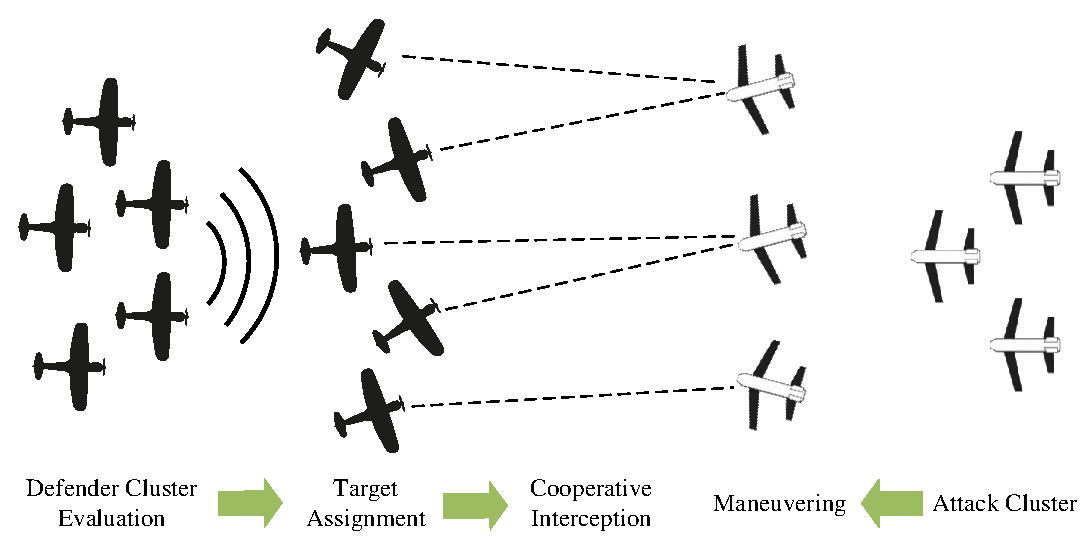
\includegraphics[width=2.8in]{fenpei.pdf}
\caption{Cluster target interception problem.}
\label{fenpei}
\end{figure}

The object of study in this paper is the fixed-wing UAV, and the interception problem is
formulated in three-dimensional space,
as shown in Fig.~\ref{jianmo} .

\begin{figure}[!t]
\centering
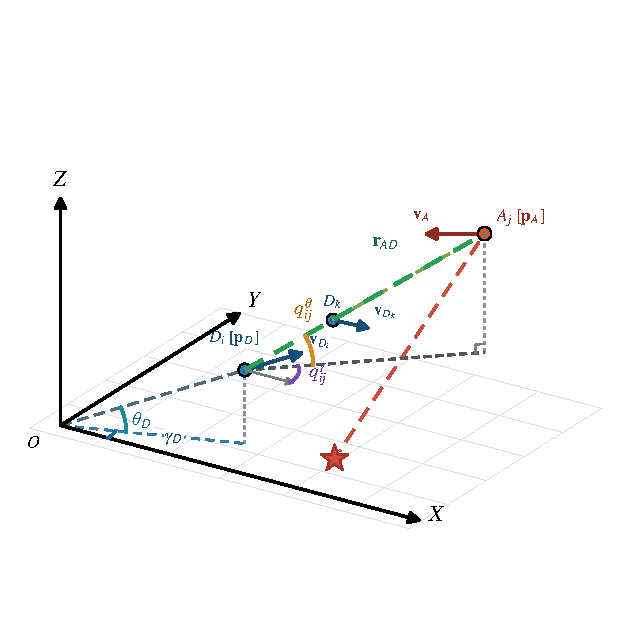
\includegraphics[width=3.3in]{pic02-3d.pdf}
\caption{Schematic diagram of confrontation and interception.}
\label{jianmo}
\end{figure}

The kinematic model of a single UAV can be simplified as
\begin{equation}
\label{yundongxue3d}
{\left\{\begin{aligned}
\dot{x}&=V\cos\theta\cos\gamma,\\
\dot{y}&=V\cos\theta\sin\gamma,\\
\dot{z}&=V\sin\theta,
\end{aligned}\right.}
\end{equation}
where %
$(x,y,z)$ are the three-dimensional position coordinates, $V$ is the velocity magnitude,
$\gamma$ is the heading angle, and $\theta$ is the flight-path angle.

In an interception mission, let $\mathbf{p}_A,\mathbf{p}_D\in\mathbb{R}^3$ and
$\mathbf{v}_A,\mathbf{v}_D\in\mathbb{R}^3$ denote the attacker and defender states. Their
three-dimensional relative geometry is
\begin{equation}
\label{gongfang3d}
{\begin{aligned}
\mathbf{r}_{AD}&=\mathbf{p}_A-\mathbf{p}_D,\qquad
r=\|\mathbf{r}_{AD}\|_2,\\
\boldsymbol{\ell}_{AD}&=\mathbf{r}_{AD}/r,\qquad
\dot{r}=\boldsymbol{\ell}_{AD}^{\top}(\mathbf{v}_A-\mathbf{v}_D).
\end{aligned}}
\end{equation}
%
where $r$ and $\boldsymbol{\ell}_{AD}$ denote the three-dimensional relative distance
and LOS unit vector, respectively. As illustrated in Fig.~\ref{jianmo},
$q_{ij}^{\gamma}$ and $q_{ij}^{\theta}$ are the corresponding LOS azimuth and elevation angles.

In the interception phase, the relationship between UAV flight state and acceleration is:
\begin{equation}
\label{guozai3d}
{\left\{\begin{aligned}
\dot{V}&=n_x g,\\
\dot{\gamma}&=\frac{n_y g}{V\cos\theta},\\
\dot{\theta}&=\frac{n_z g}{V},
\end{aligned}\right.}
\end{equation}
where $n_x$, $n_y$, and $n_z$ denote the axial, lateral, and normal
accelerations, and $g$ denotes gravitational acceleration.
In the multi-agent setting of Section~\ref{sec:cooperative_algorithm}, these variables carry
an agent subscript $i$.

During cooperative interception, the remaining impact time is defined as
\begin{equation}
\label{shijian}
t_{go}=\frac{r}{\left|\dot{r}\right|}
\end{equation}

The Zero-Effort Miss (ZEM) is defined as
\begin{equation}
\label{ZEM3d}
{\operatorname{ZEM}=\left\|\mathbf{r}_{AD}+(\mathbf{v}_A-\mathbf{v}_D)\,t_{go}\right\|_2.}
\end{equation}

\subsection{Reinforcement Learning}

Reinforcement learning (RL) is built on the Markov Decision Process (MDP), comprising state
space $\mathcal{S}$, action space $\mathcal{A}$, reward function $R$, policy $\pi$, and state
transition function $P$.
At each step, the agent selects action $a$ from state $s$, receives reward $r$, and
transitions to $s'$.
The key value functions are:
\begin{equation}
\label{RLV}
V^{\pi}(s)=E_{\pi}\left[\sum_{t=0}^{\infty}\gamma_{\mathrm{RL}}^{t}r_{t}\mid s_{0}=s\right]
\end{equation}
\begin{equation}
\label{RLQ}
Q^{\pi}(s,a)=E_{\pi}\left[\sum_{t=0}^{\infty}\gamma_{\mathrm{RL}}^{t}r_{t}\mid s_{0}=s,a_{0}=a\right]
\end{equation}
where $\gamma_{\mathrm{RL}}\in[0,1]$ is the discount factor.






\section{Target Assignment via Distributed Consensus-Based IDBO Algorithm}
\label{sec:target_assignment}

This section formulates the cooperative target assignment as a weighted bipartite matching problem and solves it via an Improved Dung Beetle Optimization (IDBO) algorithm embedded in a distributed consensus framework.

\subsection{Problem Formulation}
\label{subsec:problem_formulation}

Let $\mathcal{U} = \{u_1, u_2, \dots, u_M\}$ and $\mathcal{T} = \{t_1, t_2, \dots, t_N\}$ denote the interceptor and target sets, respectively. Figure \ref{km} illustrates the bipartite assignment structure.

\begin{figure}[!t]
\centering
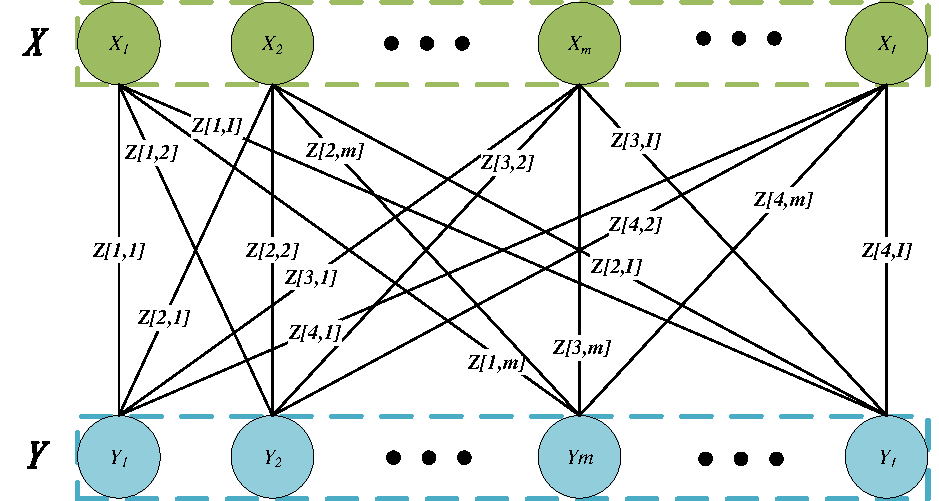
\includegraphics[width=2.5in]{KM1.pdf}
\caption{Schematic diagram of weighted dichotomy.}
\label{km}
\end{figure}

The binary decision variable $X_{ij}=1$ if UAV $u_i$ is assigned to target $t_j$ and 0 otherwise. The edge weight $P_{ij}$ quantifies the interception probability:

\begin{equation}
\label{eq:interception_probability}
P_{ij} = w_{1,\mathrm{IDBO}} \cdot P_{\text{ZEM}}(i,j) + w_{2,\mathrm{IDBO}} \cdot P_{\sigma}(i,j)
\end{equation}
where $w_{1,\mathrm{IDBO}}+w_{2,\mathrm{IDBO}}=1$, $w_{1,\mathrm{IDBO}},w_{2,\mathrm{IDBO}}\geq0$. The Zero-Effort Miss (ZEM) component is:

\begin{equation}
\label{eq:zem_prob}
P_{\text{ZEM}}(i,j) = \exp\left[-\frac{1}{2}\left(\frac{\text{ZEM}(i,j)}{\overline{\text{ZEM}}}\right)^2\right]
\end{equation}
where $\overline{\text{ZEM}} = \frac{1}{MN}\sum_{i=1}^{M}\sum_{j=1}^{N} \text{ZEM}(i,j)$.

The angular advantage component is:

\begin{equation}
\label{eq:angular_prob}
P_{\sigma}(i,j) = \exp\left[-\frac{1}{2}\left(\frac{S_{\sigma}(i,j)}{\overline{S_{\sigma}}}\right)^2\right]
\end{equation}
where $\overline{S_{\sigma}} = \frac{1}{MN}\sum_{i=1}^{M}\sum_{j=1}^{N} S_{\sigma}(i,j)$, with $S_{\sigma}(i,j) = \sqrt{(\gamma_i - q_{ij}^{\gamma})^2 + (\theta_i - q_{ij}^{\theta})^2}$ denoting the three-dimensional angular error. 
The weight $w_{1,\mathrm{IDBO}}$ prioritizes ZEM-based reachability, whereas $w_{2,\mathrm{IDBO}}$ prioritizes three-dimensional angular alignment. A sensitivity analysis of these weights is presented in Section~\ref{subsec:parameter_sensitivity}.
The objective minimizes the expected number of surviving targets. Under many-to-one assignment, the joint survival probability of target $t_j$ is the product of individual failure probabilities:

\begin{equation}
\label{eq:optimization_formulation}
\begin{aligned}
\min_{\mathbf{X}} \quad & J = \sum_{j=1}^{N} \left[ \prod_{i=1}^{M} \left(1 - P_{ij}\right)^{X_{ij}} \right] \\
\text{s.t.} \quad & \sum_{j=1}^{N} X_{ij} = 1, \quad \forall i \in \{1,\dots,M\} \\
& \sum_{i=1}^{M} X_{ij} \geq 1, \quad \forall j \in \{1,\dots,N\} \\
& \sum_{i=1}^{M} X_{ij} \leq L_{\max}, \quad \forall j \in \{1,\dots,N\} \\
& X_{ij} \in \{0,1\}, \quad \forall i,j
\end{aligned}
\end{equation}
where $\prod_{i=1}^{M} (1 - P_{ij})^{X_{ij}}$ yields the survival probability of $t_j$, which decreases geometrically with the number of assigned interceptors.


\subsection{Distributed Consensus-Based IDBO Framework}
\label{subsec:idbo_algorithm}

The IDBO algorithm solves \eqref{eq:optimization_formulation} by alternating between local metaheuristic optimization and distributed consensus-based conflict resolution. Let $\mathbf{X}^{(k)} = [x_{ij}^{(k)}] \in \{0,1\}^{M \times N}$ denote the assignment matrix at iteration $k$, where $x_{ij}^{(k)}=1$ indicates UAV $u_i$ is assigned to target $t_j$. The integrated optimization is:

\begin{equation}
\label{eq:hierarchical}
\mathcal{A}_{\text{IDBO}}^{(k+1)} = \mathcal{G}_{\text{consensus}} \circ \mathcal{F}_{\text{optimizer}} \left( \mathbf{X}^{(k)}, \boldsymbol{\Theta}^{(k)} \right)
\end{equation}
where $\mathcal{F}_{\text{optimizer}}$ denotes the improved DBO operator and $\mathcal{G}_{\text{consensus}}$ the consensus-based conflict resolver. The parameter set $\boldsymbol{\Theta}^{(k)} = \{\mathbf{A}^{(k)}, \mathbf{P}^{(k)}, \mathbf{V}^{(k)}\}$ aggregates the adversarial advantage, interception probability, and velocity matrices at iteration $k$.

Each UAV $u_i$ maintains a preference vector $\mathbf{x}_i \in [0,1]^{N}$, where $x_{ij}$ encodes the normalized affinity for target $t_j$. The fitness function balances interception efficiency against resource saturation:

\begin{equation}
\label{eq:idbo_fitness}
\begin{split}
\mathcal{F}_i(\mathbf{x}_i) =& \sum_{j=1}^{N} \sigma(x_{ij}) \cdot P_{ij} + \lambda_1 \sum_{j=1}^{N} \sigma(x_{ij}) \cdot A_{ij} \\
&- \lambda_2 \sum_{j=1}^{N} \Psi_{ij}(\mathbf{x}_i, \hat{\mathbf{X}}_{\mathcal{N}_i})
\end{split}
\end{equation}
where the three terms correspond to interception probability, adversarial advantage ($\lambda_1$-weighted), and an over-saturation penalty ($\lambda_2$-weighted). The penalty $\Psi_{ij}$ is:

\begin{equation}
\label{eq:saturation_penalty}
\begin{split}
\Psi_{ij}(\mathbf{x}_i, \hat{\mathbf{X}}_{\mathcal{N}_i}) =& \sigma(x_{ij}) \cdot \max\Biggl(0, \Biggl(\sum_{k \in \mathcal{N}_i, k \neq i} \sigma(\hat{x}_{kj}) \\
&+ \sigma(x_{ij})\Biggr) - L_{\max}\Biggr)
\end{split}
\end{equation}
where $\mathcal{N}_i$ is the neighbor set of $u_i$, $\hat{x}_{kj}$ the estimated preference of neighbor $u_k$, and $L_{\max}$ the per-target interceptor capacity. 
The penalty activates only when the estimated assignment count exceeds $L_{\max}$, steering the swarm toward capacity-feasible solutions.
In intuitive terms, each interceptor increases its preference
for targets that combine high interception likelihood with a strong
tactical advantage, while the saturation penalty redirects the local search
when neighboring preferences indicate that a target has reached its
allocation capacity.


The adversarial advantage $A_{ij}$ fuses temporal, energetic, and geometric factors:

\begin{equation}
\label{eq:adversarial_advantage}
\begin{split}
A_{ij} =& \exp\left(-\frac{\Delta t_{ij}}{T_{\max}}\right) \cdot \left(1 - \frac{\|\mathbf{v}_i - \mathbf{v}_j\|_2}{v_{\max}}\right) \\
&\cdot \max\left(0,
\frac{\mathbf{v}_i^{\top}(\mathbf{p}_j-\mathbf{p}_i)}
{\|\mathbf{v}_i\|_2\,\|\mathbf{p}_j-\mathbf{p}_i\|_2}\right) \\
&- \sum_{k\neq i} \frac{P_{kj}}{P_{ij} + P_{kj}} \cdot \sigma(\hat{x}_{kj})
\end{split}
\end{equation}
where $\Delta t_{ij}$ is the estimated time-to-intercept; $\mathbf{p}_i=[x_i,y_i,z_i]^\top$ and $\mathbf{v}_i=[\dot{x}_i,\dot{y}_i,\dot{z}_i]^\top$ denote the three-dimensional position and velocity vectors of interceptor $u_i$, while $\mathbf{p}_j=[x_j,y_j,z_j]^\top$ and $\mathbf{v}_j=[\dot{x}_j,\dot{y}_j,\dot{z}_j]^\top$ denote those of target $t_j$; and $v_{\max}$ is the maximum reference speed used for normalization. 
The normalized inner product is the cosine of the three-dimensional angle between the interceptor velocity and the LOS to target $t_j$; the maximum operator assigns zero geometric advantage when the target lies outside the interceptor's forward hemisphere. The three multiplicative factors encode temporal, energetic, and geometric advantage, respectively, while the subtracted term penalizes competition from other interceptors with high preferences for the same target.



The IDBO update mechanism enhances the standard DBO through four adversarial-information-driven operations:

\begin{align}
\text{Rolling:} \quad & \mathbf{x}_i^{(t+1)} = \mathbf{x}_i^{(t)} + \alpha \cdot \nabla_{\mathbf{x}_i} \mathcal{F}_i(\mathbf{x}_i^{(t)}) \circ \mathbf{A}_i \nonumber \\
& \quad + \beta \cdot \boldsymbol{\xi}_i \cdot \mathrm{e}^{-t/T} \label{eq:rolling_update} \\
\text{Dancing:} \quad & \mathbf{x}_i^{(t+1)} = \mathbf{x}_i^{(t)} \odot \exp\left(\gamma_{\mathrm{IDBO}} \cdot \tanh(\mathbf{A}_i - \bar{A}_i)\right) \nonumber \\
& \quad + \mathbf{n}_i, \quad \mathbf{n}_i \sim \mathcal{N}(0, \sigma_d^2 \mathbf{I}) \label{eq:dancing_update} \\
\text{Breeding:} \quad & \mathbf{x}_i^{(t+1)} = \mathbf{x}_i^{(t)} + \delta \cdot \left(\mathbf{x}_{\text{best}}^{(t)} - \mathbf{x}_i^{(t)}\right) \odot \mathbf{A}_i \nonumber \\
& \quad + \delta' \cdot \left(\mathbf{x}_{\text{second}}^{(t)} - \mathbf{x}_i^{(t)}\right) \label{eq:breeding_update} \\
\text{Stealing:} \quad & \mathbf{x}_i^{(t+1)} = \mathbf{x}_i^{(t)} \nonumber \\
& \quad + \eta_{\mathrm{IDBO}} \cdot \sum_{k \in \mathcal{K}_i} \frac{A_{ij}}{\sum_{l \in \mathcal{K}_i} A_{lj}} \cdot \left(\mathbf{x}_k^{(t)} - \mathbf{x}_i^{(t)}\right) \label{eq:stealing_update}
\end{align}
where $\mathbf{A}_i = [A_{i1}, A_{i2}, \dots, A_{iN}]^\top$, $\bar{A}_i$ is the mean of $\mathbf{A}_i$, $\boldsymbol{\xi}_i$ and $\mathbf{n}_i$ are random vectors, $\mathcal{K}_i$ represents UAVs competing for the same targets as $u_i$, and $\alpha, \beta, \gamma_{\mathrm{IDBO}}, \delta, \delta', \eta_{\mathrm{IDBO}}$ are adaptive coefficients that decay linearly with iteration $t$. 
The coefficients
$\alpha,\beta,\gamma_{\mathrm{IDBO}},\delta,\delta',
\eta_{\mathrm{IDBO}}$, together with the dancing-noise scale $\sigma_d$,
follow the common linear schedule $c_t=c_0(1-t/T)$, where $T$ denotes the
local IDBO search horizon. During each local search, the candidate
preferences are projected onto $[0,1]^N$, and the best-so-far candidate is
retained unless a strictly better candidate is obtained. The coefficient
schedule progressively attenuates both the directed update terms and the
stochastic perturbations. In particular, the rolling perturbation
$\beta\boldsymbol{\xi}_i\mathrm{e}^{-t/T}$ and the dancing perturbation
$\mathbf{n}_i\sim\mathcal{N}(0,\sigma_d^2\mathbf{I})$ vanish as $t$
approaches $T$, suppressing late-stage fluctuations in the preference
population. The schedule therefore satisfies the vanishing-gain condition
$c_t\to0$ used in Robbins--Monro-type stochastic approximation
\cite{robbins1951stochastic}. At $c_T=0$, the four update operators reduce
to the identity map, while elitist retention prevents the incumbent from
being replaced by an inferior candidate. Consequently, once no strictly
improving candidate is generated, the retained solution remains invariant
and constitutes a stable fixed point of the implemented local search.
Continuous preferences are binarized via advantage-adaptive thresholding:

\begin{equation}
\label{eq:thresholding}
X_{ij} = 
\begin{cases}
1, & \text{if } \sigma(x_{ij}) > \tau \cdot \left(1 + \frac{A_{ij}}{\max_k A_{ik}}\right) \\
0, & \text{otherwise}
\end{cases}
\end{equation}
where $\tau \in (0,1)$ is a base threshold. Each UAV maintains a bundle $\mathcal{B}_i$, bid vector $\mathbf{c}_i = [c_{i1}, \dots, c_{iN}]$, winner list $\mathbf{z}_i = [z_{i1}, \dots, z_{iN}]$, and timestamp vector $\mathbf{y}_i = [y_{i1}, \dots, y_{iN}]$. The bid for target $t_j$ governs the distributed auction:

\begin{equation}
\label{eq:bid_formulation}
c_{ij} = \mathcal{F}_i(\mathbf{x}_i) \cdot \sigma(x_{ij}) \cdot \exp\left(\frac{A_{ij} - \bar{A}_i}{\sigma_A}\right)
\end{equation}
where $\bar{A}_i$ and $\sigma_A$ are the mean and standard deviation of $u_i$'s adversarial advantages. The fitness--preference product captures local assignment quality, while the exponential term amplifies bids for targets where $u_i$ holds above-average advantage. To support cooperative saturation attacks, the consensus mechanism employs top-$K$ bidding. Each UAV maintains a winner list $\mathcal{Z}_{j} = \{(u_k, c_{kj})\}$ for $t_j$, containing up to $L_{\max}$ highest bids:

\begin{equation}
\label{eq:cbba_update}
\mathcal{Z}_{j}^{(k+1)} = \text{Top}_{L_{\max}} \left( \mathcal{Z}_{j}^{(k)} \cup \bigcup_{l \in \mathcal{N}_i} \mathcal{Z}_{j,l}^{(k)} \cup \{(u_i, c_{ij}^{(k+1)})\} \right)
\end{equation}
where $\text{Top}_{L_{\max}}(\cdot)$ retains the $L_{\max}$ highest-bid entries. UAV $u_i$ secures a slot for $t_j$ if $|\mathcal{Z}_{j}| < L_{\max}$ or its bid exceeds $\min_{(u_k, c_{kj}) \in \mathcal{Z}_{j}} c_{kj}$, thereby displacing the weakest contributor and prioritizing the most capable interceptors.
Equations~\eqref{eq:thresholding}--\eqref{eq:cbba_update}
convert the continuous preferences into local assignment candidates. Each
consensus update exchanges the current bids among neighboring interceptors
and retains at most the $L_{\max}$ strongest bids for each target. Once the
local search has stabilized and the bids no longer change, repeated consensus
updates propagate the winner information through the connected network and
bring the local winner lists into agreement.

As depicted in the procedural flowchart (Fig.~\ref{fig:idbo_flowchart}), the algorithm iterates over three interleaved phases—local optimization (Eqs.~\ref{eq:rolling_update}--\ref{eq:stealing_update}), consensus resolution (Eqs.~\ref{eq:thresholding}--\ref{eq:cbba_update}), and advantage update—until convergence:

\begin{align}
\text{Phase 1: } & \mathbf{x}_i^{(k+1)} = \mathcal{F}_{\text{optimizer}}\left(\mathbf{x}_i^{(k)}, \mathcal{F}_i, \mathbf{A}_i^{(k)}, \mathbf{P}^{(k)}\right) \label{eq:phase1} \\
\text{Phase 2: } & \{\mathbf{z}_i^{(k+1)}, \mathcal{B}_i^{(k+1)}\} = \nonumber \\ 
& \mathcal{G}_{\text{consensus}}\left(\{\sigma(\mathbf{x}_i^{(k+1)})\}, \{\mathbf{c}_i^{(k+1)}\}, \{\mathbf{y}_i^{(k)}\}\right) \label{eq:phase2} \\
\text{Phase 3: } & \mathbf{A}_i^{(k+1)} = \mathcal{H}\left(\mathbf{z}_i^{(k+1)}, \mathcal{B}_i^{(k+1)}, \mathbf{V}_i^{(k+1)}, \mathbf{V}_T^{(k+1)}\right) \label{eq:phase3}
\end{align}

\begin{figure}[!t]
\centering
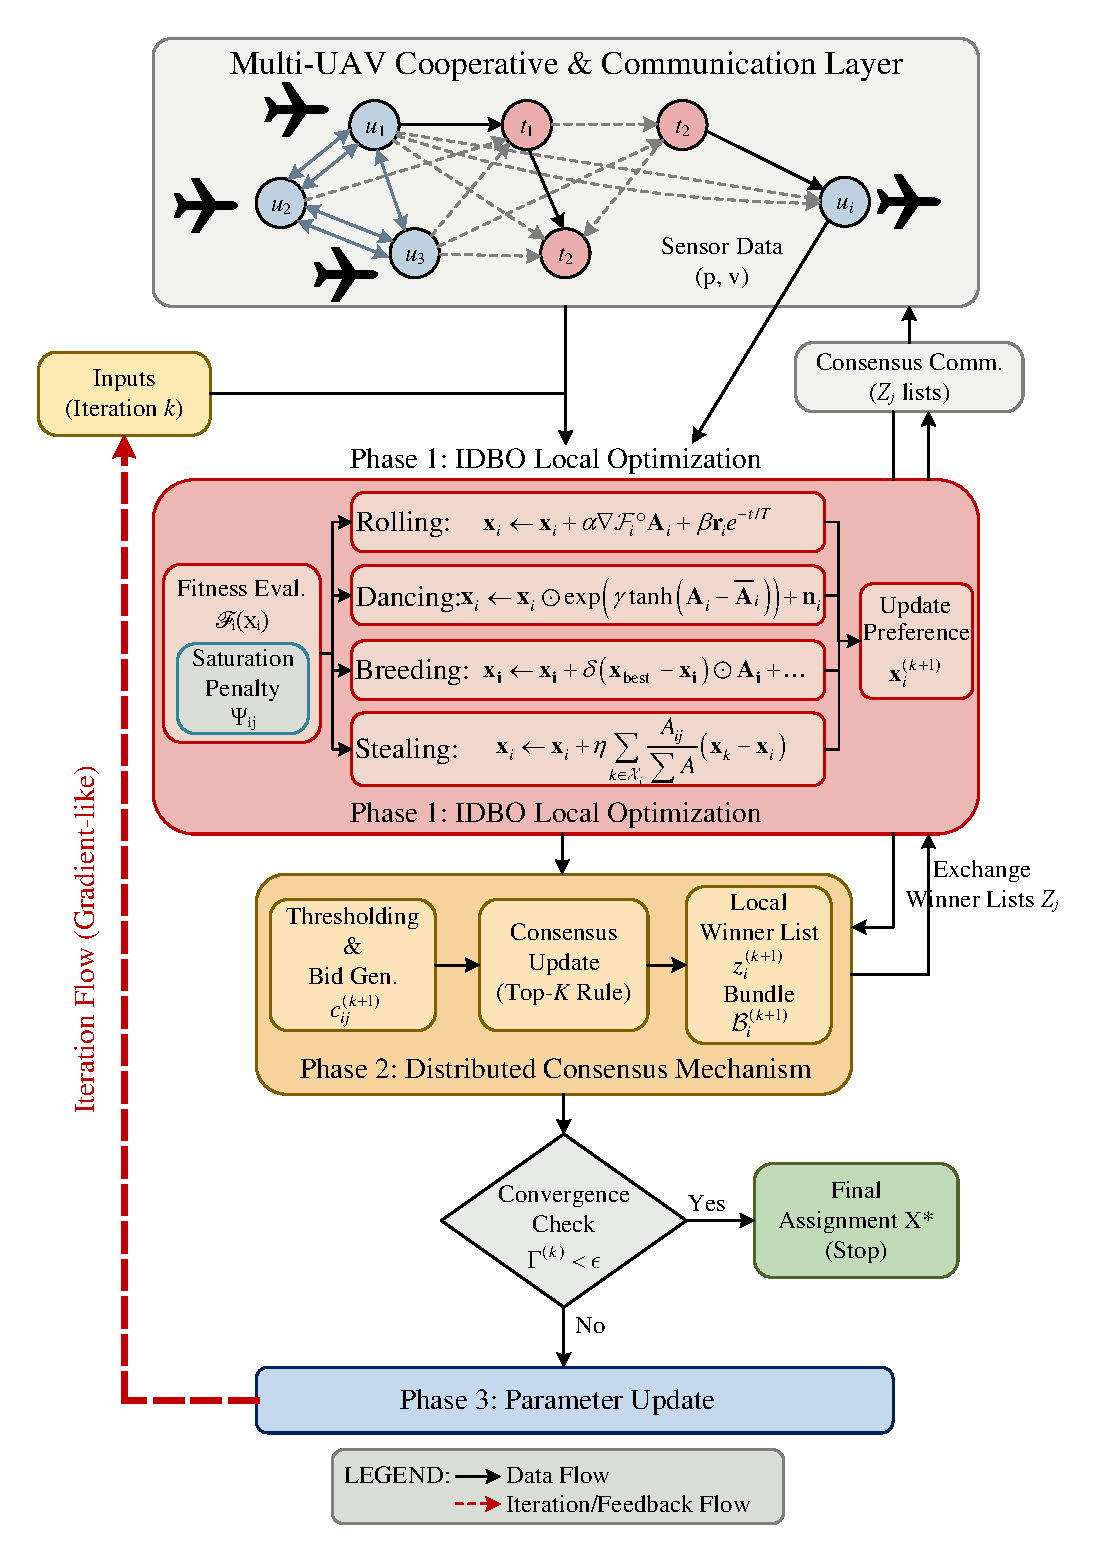
\includegraphics[width=3.2in]{assignment.pdf}
\caption{Flowchart of the distributed consensus-based IDBO algorithm, illustrating the algorithmic iteration flow across local metaheuristic optimization, auction-based consensus, and adversarial information updates.}
\label{fig:idbo_flowchart}
\end{figure}

Here, $\mathcal{H}$ updates adversarial advantages given the consensus assignment and velocity vectors $\mathbf{V}_i$, $\mathbf{V}_T$. Following the iteration flow in Fig.~\ref{fig:idbo_flowchart}, convergence is declared when the swarm-wide assignment disagreement falls below $\epsilon_{\mathrm{IDBO}}$:

\begin{equation}
\label{eq:convergence}
\Gamma^{(k)} = \frac{1}{M} \sum_{i=1}^{M} \left\| \mathbf{z}_i^{(k)} - \frac{1}{|\mathcal{N}_i|} \sum_{j \in \mathcal{N}_i} \mathbf{z}_j^{(k)} \right\|_0 < \epsilon_{\mathrm{IDBO}}
\end{equation}
where $\|\cdot\|_0$ counts disagreeing entries and $\epsilon_{\mathrm{IDBO}}$ is a convergence threshold.  
% Three properties characterize this iteration under a connected communication graph with bounded message delay and elitist retention of best-so-far solutions. First, the \emph{incumbent} (best-so-far) swarm fitness $\Phi_{\mathrm{best}}^{(k)}=\max_{k'\le k}\sum_{i=1}^{M}\mathcal{F}_i(\mathbf{x}_i^{(k')})$ is non-decreasing by construction, and because the decaying schedule $c_t=c_0(1-t/T)$ drives the operators' stochastic amplitude to zero while retaining an ascent direction, the working assignment settles at a fixed point rather than orbiting it---the standard Robbins--Monro condition for stochastic-approximation convergence~\cite{robbins1951stochastic}. Second, the auction-based consensus phase~\eqref{eq:bid_formulation}--\eqref{eq:cbba_update} inherits the guarantees of the consensus-based bundle algorithm~\cite{choi2009consensus}: with a diminishing-marginal-gain (submodular) score it reaches a conflict-free assignment in at most $N\!\cdot\!D$ communication rounds ($D$: graph diameter). Third, the resulting fixed point $\mathbf{X}^\ast$ is $\epsilon_{\mathrm{IDBO}}$-\emph{stable}---no interceptor can raise its own fitness by more than $\epsilon_{\mathrm{IDBO}}$ through a unilateral reassignment, $\mathcal{F}_i(\mathbf{x}_i^\ast)\ge\mathcal{F}_i(\mathbf{x}_i')-\epsilon_{\mathrm{IDBO}}$ for all $\mathbf{x}_i'\in\mathcal{X}_i$ and all $i$, which follows directly from the auction best-response at the converged bid prices~\cite{choi2009consensus}. The empirical convergence of the swarm-disagreement metric $\Gamma^{(k)}$ and the near-linear growth of consensus rounds with $D$ are reported in the supplementary response material. The complete per-interceptor procedure is summarized in Algorithm~\ref{alg:idbo}.}
The local optimization and consensus phases have distinct limiting
properties. The diminishing coefficient schedule and elitist retention
stabilize the local search as described above. For the consensus phase,
suppose that the bids remain fixed, the communication graph is connected
with diameter $D$, messages are delivered with bounded delay, and equal bids
are resolved deterministically. Under these conditions, the top-$L_{\max}$
winner information propagates by at least one communication hop in each
successful round. Consequently, all interceptors obtain the same winner list
for each target after at most $D$ successful communication rounds. Bounded
delay increases the elapsed consensus time but does not alter the resulting
winner lists. Once agreement is reached, further applications of
\eqref{eq:cbba_update} leave the winner lists unchanged; hence, they form a
consensus fixed point. Each list contains at most $L_{\max}$ interceptors, and,
provided that a feasible assignment exists, the subsequent conflict-resolution
step enforces the constraints in \eqref{eq:optimization_formulation}. Here,
$\epsilon_{\mathrm{IDBO}}$ specifies the numerical tolerance for winner-list
disagreement.



\begin{algorithm}[!t]
\caption{IDBO Target Assignment}
\label{alg:idbo}
\begin{algorithmic}[1]
\REQUIRE Interceptor and target sets $\mathcal{U},\mathcal{T}$; engagement states; communication graph; capacity $L_{\max}$; local population size $N_{\mathrm{pop}}$; local search horizon $T$; tolerance $\epsilon_{\mathrm{IDBO}}$
\ENSURE Feasible consensus assignment $\mathbf{X}^{\ast}$
\STATE Each interceptor $u_i$ initializes a local preference population, assignment replica, bid/winner records, and timestamps; set $k\!\leftarrow\!0$
\REPEAT
  \STATE Evaluate $\mathbf{P}$ using~\eqref{eq:interception_probability} and the adversarial advantages using~\eqref{eq:adversarial_advantage}
  \FOR{$t=1$ to $T$}
    \STATE Set the linearly decaying coefficients $c_t=c_0(1-t/T)$ for the four IDBO operators
    \STATE Evaluate all local candidates with $\mathcal{F}_i$~\eqref{eq:idbo_fitness}
    \STATE Generate candidates using the rolling, dancing, breeding, and stealing operators according to \eqref{eq:rolling_update}--\eqref{eq:stealing_update}
    \STATE Project the candidate preferences onto $[0,1]^N$ and retain the current best candidate unless a strictly better candidate is obtained
  \ENDFOR
  \STATE Select and binarize the best local preference using~\eqref{eq:thresholding}; compute the target bids using~\eqref{eq:bid_formulation}
  \STATE Exchange local records with $\mathcal{N}_i$, update the top-$L_{\max}$ winner lists using~\eqref{eq:cbba_update}, and resolve assignment conflicts subject to the constraints in~\eqref{eq:optimization_formulation}
  \STATE Update the local feasible assignment replica and adversarial information; evaluate consensus disagreement; $k\!\leftarrow\!k+1$
\UNTIL{the disagreement falls below $\epsilon_{\mathrm{IDBO}}$}
\STATE Set $\mathbf{X}^{\ast}$ to the common feasible assignment replica
\STATE \textbf{return} $\mathbf{X}^{\ast}$
\end{algorithmic}
\end{algorithm}

The per-UAV per-iteration complexity decomposes as:

\begin{equation}
\label{eq:complexity}
C_{\text{total}} = O(T \cdot P \cdot N^2) + O(N \cdot |\mathcal{N}_i|) + O(N)
\end{equation}
where $T$ is the IDBO iteration count, $P = O(N)$ the population size, and $|\mathcal{N}_i|$ the neighborhood size. The three terms account for optimization, consensus communication, and advantage update, respectively. Communication cost is $O(N \cdot |\mathcal{N}_i|)$ and memory is $O(P \cdot N + N)$ per UAV. 
% Because the target set faced by each interceptor and its neighborhood size $|\mathcal{N}_i|$ are fixed by the engagement and the communication topology rather than by the swarm size $M$, the per-UAV per-iteration cost above is independent of $M$; the total per-round cost of the swarm therefore grows only linearly with $M$. Scalability is governed not by this arithmetic cost but by how fast the distributed consensus in \eqref{eq:convergence} settles. Under a connected graph with a per-hop communication latency $T_{\mathrm{comm}}$, each target's winning bids propagate across the network in at most $D$ hops ($D$: graph diameter), so the wall-clock time to reach consensus scales as $O(N\!\cdot\!D\!\cdot\!T_{\mathrm{comm}})$. Empirically, the consensus time increases approximately linearly with the communication delay and with $D$. Bounded delay slows but does not prevent convergence for a static assignment snapshot; under time-varying cooperative deflection, the consensus time must remain shorter than the reallocation interval. Detailed complexity, scalability, and communication-delay measurements are reported in Section~\ref{subsec:assignment_results}.}
As $M$ and $N$ increase together, the overall computational workload
also increases, as quantified by the scalability results in
Section~\ref{subsec:assignment_results}. Communication-side scalability is
governed by the convergence efficiency of the distributed consensus process.
Once the bids have stabilized, the winner lists for all $N$ targets are
exchanged together and propagate through a connected graph of diameter $D$
within at most $D$ successful communication rounds. The corresponding
communication time scales as $O(DT_{\mathrm{comm}})$ under bounded per-hop
delay $T_{\mathrm{comm}}$, while the per-round communication processing cost
is $O(N|\mathcal{N}_i|)$. The experiments in
Section~\ref{subsec:assignment_results} show that increasing communication
delay increases both the mean communication steps and the consensus time,
while all tested cases reach common top-$L_{\max}$ winner lists.





%% ===========================================================
\section{ART-MAPPO: Attention-Residual and Trust-Aware MAPPO for Cooperative Swarm Interception}
\label{sec:cooperative_algorithm}

% Building on the distributed consensus-based IDBO target assignment, we propose the Attention-Residual and Trust-aware MAPPO (ART-MAPPO) algorithm for the cooperative guidance of defending UAV swarms under the Centralized Training with Decentralized Execution (CTDE) paradigm. ART-MAPPO augments the standard MAPPO framework with three synergistic modules: a kinematics-aware attention-residual network for extracting cross-coupled engagement features, a trust-modulated exploration mechanism for discovering cooperative tactics within the safe flight envelope, and a dual-clip PPO with adaptive KL penalty for constraining guidance command variations against actuator saturation.

Building on the distributed consensus-based IDBO target assignment, we propose
the Attention-Residual and Trust-aware MAPPO (ART-MAPPO) algorithm for the
cooperative guidance of defending UAV swarms under the Centralized Training
with Decentralized Execution (CTDE) paradigm. ART-MAPPO augments the standard
MAPPO framework with two
task-oriented modules: a kinematics-aware attention-residual network for
extracting cross-coupled engagement features and a
trust-modulated exploration mechanism for discovering cooperative tactics
within the safe flight envelope. Dual-Clip PPO and adaptive KL regularization are used to
stabilize policy updates during training.

\subsection{Enhanced Situational Awareness via Attention-Residual Network}
\label{subsec:attention_residual}

The highly dynamic nature of swarm interception requires interceptors to process complex, coupled kinematic states. Let $\mathbf{o}_i^{(t)} \in \mathbb{R}^{n_o}$ denote the observation vector for interceptor $i$ at time step $t$, as defined in Section~\ref{subsec:state_reward}. A base feature encoder $f_{\mathrm{enc}}$, comprising a two-layer MLP with hidden dimension $d_{\mathrm{enc}}$ and Layer Normalization, projects the raw observation into a high-dimensional latent space:
\begin{equation}
\label{eq:encoder}
\begin{split}
\mathbf{h}^{(0)} =& \operatorname{LN}\Bigl(\operatorname{ReLU}\bigl(\mathbf{o}_i^{(t)}\mathbf{W}_{\mathrm{enc}}^{(1)} + \mathbf{b}_{\mathrm{enc}}^{(1)}\bigr) \\
&\cdot \mathbf{W}_{\mathrm{enc}}^{(2)} + \mathbf{b}_{\mathrm{enc}}^{(2)}\Bigr) \in \mathbb{R}^{d}
\end{split}
\end{equation}
where $\mathbf{W}_{\mathrm{enc}}^{(1)} \in \mathbb{R}^{n_o \times d_{\mathrm{enc}}}$ and $\mathbf{W}_{\mathrm{enc}}^{(2)} \in \mathbb{R}^{d_{\mathrm{enc}} \times d}$ are learnable projection matrices.

\emph{1) Kinematics-Aware Multi-Head Attention:} To capture the nonlinear spatio-temporal coupling among engagement variables (e.g., the interdependence of the LOS azimuth and elevation rates $\dot{q}^{\gamma}$ and $\dot{q}^{\theta}$ with time-to-go synchronization), we reshape $\mathbf{h}^{(0)}$ into a sequence of $n_o$ feature tokens $\mathbf{H}^{(0)} \in \mathbb{R}^{n_o \times (d/n_o)}$ and apply multi-head self-attention. For each head $j \in \{1, \dots, H\}$, the query, key, and value projections are:
\begin{equation}
\label{eq:qkv}
\mathbf{Q}_j = \mathbf{H}^{(0)}\mathbf{W}_j^{Q}, \quad \mathbf{K}_j = \mathbf{H}^{(0)}\mathbf{W}_j^{K}, \quad \mathbf{V}_j = \mathbf{H}^{(0)}\mathbf{W}_j^{V}
\end{equation}
where $\mathbf{W}_j^{Q}, \mathbf{W}_j^{K} \in \mathbb{R}^{(d/n_o) \times d_k}$ and $\mathbf{W}_j^{V} \in \mathbb{R}^{(d/n_o) \times d_v}$, with $d_k = d_v = d/H$. The scaled dot-product attention for head $j$, incorporating an observability mask $\mathbf{M} \in \mathbb{R}^{n_o \times n_o}$, is:
\begin{align}
\mathbf{A}_j &= \mathrm{softmax}\!\left(\frac{\mathbf{Q}_j\mathbf{K}_j^\top}{\sqrt{d_k}} + \mathbf{M}\right) \in \mathbb{R}^{n_o \times n_o} \label{eq:attention} \\
\mathrm{head}_j &= \mathbf{A}_j\mathbf{V}_j \in \mathbb{R}^{n_o \times d_v} \nonumber
\end{align}
where $M_{u,v} = -\infty$ isolates unobservable kinematic channels (e.g., LOS rate during sensor blanking) and $M_{u,v} = 0$ permits information flow. The multi-head outputs are concatenated, projected, and added back via a residual shortcut:
\begin{equation}
\label{eq:mha_out}
\begin{split}
\mathbf{h}_{\mathrm{attn}} =& \mathbf{h}^{(0)} + \mathrm{Dropout}_{p}\Bigl(\operatorname{Flatten}\bigl( \\
&\left[\mathrm{head}_1 \| \cdots \| \mathrm{head}_H\right]\bigr) \mathbf{W}^{O}\Bigr)
\end{split}
\end{equation}
where $\mathbf{W}^{O} \in \mathbb{R}^{(n_o d) \times d}$  is the output projection and $\operatorname{Flatten}(\cdot)$ reshapes the concatenated token sequence into $\mathbb{R}^{n_o d}$.
Each row of $\mathbf{A}_j$ specifies how the observable
kinematic features contribute to the update of one feature token. After the
head outputs are concatenated and flattened, $\mathbf{W}^{O}$ maps the
attended information from all feature tokens back to the $d$-dimensional
latent space for residual fusion with $\mathbf{h}^{(0)}$.
The residual connection ensures that primitive flight-state components propagate losslessly to downstream layers.

\emph{2) Residual Block with Layer Normalization:} To deepen the nonlinear representational capacity without gradient vanishing---a critical issue when extreme acceleration commands produce large-magnitude gradients---a stack of $L$ residual blocks follows the attention module. For the $\ell$-th block ($\ell \in \{1, \dots, L\}$) with input $\mathbf{h}^{(\ell)}$ (where $\mathbf{h}^{(1)} = \mathbf{h}_{\mathrm{attn}}$), the forward pass is:
\begin{align}
\mathbf{z}_1^{(\ell)} &= \operatorname{ReLU} \left( \operatorname{LN}_1^{(\ell)} \left( \mathbf{h}^{(\ell)}\mathbf{W}_1^{(\ell)} + \mathbf{b}_1^{(\ell)} \right) \right) \label{eq:res_block_inner1} \\
\mathbf{z}_2^{(\ell)} &= \operatorname{LN}_2^{(\ell)} \left( \mathbf{z}_1^{(\ell)}\mathbf{W}_2^{(\ell)} + \mathbf{b}_2^{(\ell)} \right) \label{eq:res_block_inner2} \\
\mathbf{h}^{(\ell+1)} &= \operatorname{ReLU} \left( \mathbf{z}_2^{(\ell)} + \mathbf{h}^{(\ell)} \right) \label{eq:res_block_out}
\end{align}
where $\mathbf{W}_1^{(\ell)}, \mathbf{W}_2^{(\ell)} \in \mathbb{R}^{d \times d}$ are orthogonally initialized. 
The nonlinear branch refines the attended representation, while
the shortcut carries the incoming engagement features directly to the next
block. This structure reduces the need to reconstruct unchanged kinematic
information at every layer.
The identity shortcut yields the Jacobian:
\begin{equation}
\label{eq:jacobian}
\begin{split}
\frac{\partial \mathbf{h}^{(\ell+1)}}{\partial \mathbf{h}^{(\ell)}} =& \operatorname{diag}\!\left(\mathbb{I}\!\left[\mathbf{z}_2^{(\ell)} + \mathbf{h}^{(\ell)} > \mathbf{0}\right]\right) \\
&\cdot \left(\mathbf{I} + \frac{\partial \mathbf{z}_2^{(\ell)}}{\partial \mathbf{h}^{(\ell)}}\right)
\end{split}
\end{equation}
Since the ReLU gate preserves the identity component on active units, gradient norms satisfy $\left\|\frac{\partial \mathbf{h}^{(\ell+1)}}{\partial \mathbf{h}^{(\ell)}}\right\| \geq \left\|\operatorname{diag}(\mathbb{I}[\cdot])\right\| > 0$, preventing vanishing gradients across $L$ blocks.

\emph{3) End-to-End Guidance Command Generation:} The refined feature $\mathbf{h}^{(L+1)}$ is fed into a GRU cell to integrate temporal engagement history:
\begin{equation}
\label{eq:gru}
\mathbf{c}_t = \operatorname{GRU}\!\left(\mathbf{h}^{(L+1)},\, \mathbf{c}_{t-1};\, \mathbf{W}_{\mathrm{GRU}}\right), \quad \mathbf{c}_t \in \mathbb{R}^{d_{\mathrm{rnn}}}
\end{equation}
where $\mathbf{W}_{\mathrm{GRU}}$ denotes the GRU parameters and $\mathbf{c}_{t-1}$ is the hidden state from the previous guidance step. The actor network then parameterizes a diagonal Gaussian over the continuous acceleration action space:
\begin{equation}
\label{eq:actor_dist}
\begin{split}
\pi_{\boldsymbol{\vartheta}_i}\!\left(\mathbf{a}_i \mid \mathbf{o}_i^{(t)}\right) &= \mathcal{N}\!\left(\boldsymbol{\mu}_{\boldsymbol{\vartheta}_i}(\mathbf{c}_t),\; \operatorname{diag}\!\left(\boldsymbol{\sigma}_{\boldsymbol{\vartheta}_i}^2(\mathbf{c}_t)\right)\right) \\
\mathbf{a}_i &= [n_{x_i},\,n_{y_i},\,n_{z_i}]^\top \in \mathcal{A}\subset\mathbb{R}^3
\end{split}
\end{equation}
where $\boldsymbol{\mu}_{\boldsymbol{\vartheta}_i}, \boldsymbol{\sigma}_{\boldsymbol{\vartheta}_i}^2: \mathbb{R}^{d_{\mathrm{rnn}}} \to \mathbb{R}^3$ are linear output heads. 
The policy mean specifies the nominal three-axis acceleration
command, while the diagonal variance controls the spread of the sampled
commands.
The three-dimensional acceleration action is clipped to the feasible envelope $\mathcal{A}$ after sampling. Concurrently, the centralized critic shares the same attention-residual backbone but receives the concatenated global state:
\begin{equation}
\label{eq:critic_input}
s_t = \left[\mathbf{o}_1^{(t)} \| \mathbf{o}_2^{(t)} \| \cdots \| \mathbf{o}_M^{(t)}\right] \in \mathbb{R}^{M \cdot n_o}
\end{equation}
to produce the state-value estimate $V_\phi(s_t) \in \mathbb{R}$, enabling centralized advantage computation during training while each actor executes independently from local observations $\mathbf{o}_i^{(t)}$ at deployment.

\subsection{Trust-Modulated Tactical Exploration}
\label{subsec:trust_exploration}

Based on the high-fidelity features extracted by the attention-residual backbone, we introduce a trust-based mechanism to dynamically modulate the exploration policy. This mechanism mathematically balances the exploitation of known guidance laws against the discovery of complex cooperative tactics (e.g., flanking or simultaneous impact).

\emph{1) Trust Evolution:} Let $R_i^{(k)} = \sum_{t=0}^{T} \gamma_{\mathrm{RL}}^t r_i^{(t)}$ be the discounted cumulative return of interceptor $i$ in episode $k$, where $\gamma_{\mathrm{RL}} \in (0,1)$ is the RL discount factor (distinct from the heading angle $\gamma_{D_i}$) and $T$ is the episode horizon. The swarm-level running statistics are maintained as exponential moving averages:
\begin{align}
\mu_R &\leftarrow (1-\rho)\,\mu_R + \rho\,\frac{1}{M}\sum_{i=1}^{M} R_i^{(k)} \label{eq:running_stats_mu} \\
\sigma_R^2 &\leftarrow (1-\rho)\,\sigma_R^2 + \rho\,\frac{1}{M}\sum_{i=1}^{M}\!\left(R_i^{(k)} - \mu_R\right)^2 \label{eq:running_stats_sigma}
\end{align}
where $\rho \in (0,1)$ is the statistics update rate. The normalized relative performance of interceptor $i$ is then:
\begin{equation}
\label{eq:trust_normalized}
\tilde{R}_i^{(k)} = \frac{R_i^{(k)} - \mu_R}{\sqrt{\sigma_R^2 + \epsilon_0}}
\end{equation}
where $\epsilon_0 > 0$ is a numerical stabilizing constant. The trust level $\mathcal{T}_i^{(k)} \in (0,1)$ evolves via first-order exponential smoothing with a sigmoid activation:
\begin{equation}
\label{eq:trust_evolution}
\mathcal{T}_i^{(k+1)} = (1-\alpha_T)\,\mathcal{T}_i^{(k)} + \alpha_T\,\sigma\!\left(\tau_T \tilde{R}_i^{(k)}\right)
\end{equation}
where $\sigma(x)=1/(1+e^{-x})$, $\alpha_T\in(0,1)$ is the trust update rate,
and $\tau_T>0$ is the temperature parameter controlling the sensitivity of
trust to performance deviations.
The sigmoid term maps the normalized relative return
$\tilde{R}_i^{(k)}$ to a bounded performance reference in $(0,1)$.
Equation~\eqref{eq:trust_evolution} combines the previous trust level and
the current performance reference with the weights $1-\alpha_T$ and
$\alpha_T$, respectively, yielding a smoothed trust estimate. The
smoothing process tracks changes in relative performance while attenuating
episode-to-episode return fluctuations. Sustained above-average returns
keep the performance reference above $0.5$ and bias the smoothed trust
estimate toward a correspondingly higher level, thereby reducing the
probability assigned to the guided exploratory policy; sustained
below-average returns produce the opposite allocation.


\emph{2) Blended Exploration Policy:} The final action for interceptor $i$ is drawn from a two-component mixture: with probability $1-\beta(\mathcal{T}_i)$ from the learned policy, and with probability $\beta(\mathcal{T}_i)$ from a structured heuristic distribution, i.e.,
\begin{equation}
\label{eq:exploration_policy}
\mathbf{a}_i \sim \begin{cases} \pi_{\boldsymbol{\vartheta}_i}(\cdot \mid \mathbf{o}_i^{(t)}) & \text{with prob. } 1 - \beta(\mathcal{T}_i) \\ \pi_{\mathrm{guided}}^{i}(\cdot \mid \mathbf{o}_i^{(t)}) & \text{with prob. } \beta(\mathcal{T}_i) \end{cases}
\end{equation}
where the modulation factor $\beta(\mathcal{T}_i) = 1 - \mathcal{T}_i \in (0,1)$ is monotonically decreasing in trust. The heuristic distribution $\pi_{\mathrm{guided}}^{i}$ is a discrete mixture over three tactically informative actions within the feasible command space $\mathcal{A} = [n_{x}^{\min},n_{x}^{\max}] \times [n_{y}^{\min},n_{y}^{\max}] \times [n_{z}^{\min},n_{z}^{\max}]$:
\begin{equation}
\label{eq:guided}
\begin{split}
\pi_{\mathrm{guided}}^{i}(\mathbf{a}_i \mid \mathbf{o}_i^{(t)}) =& \omega_1\,\delta(\mathbf{a}_i - \mathbf{a}_{\mathrm{opt}}) + \omega_2\,\delta(\mathbf{a}_i - \mathbf{a}_{\mathrm{probe}}) \\
&+ \omega_3\,\mathcal{U}(\mathcal{A}), \quad \sum_{k=1}^3\omega_k=1
\end{split}
\end{equation}
Here, $\mathbf{a}_{\mathrm{opt}} = \arg\max_{\mathbf{a} \in \mathcal{A}} Q_\phi(\mathbf{o}_i^{(t)}, \mathbf{a})$ mimics the classical proportional navigation command for exploitation, $\mathbf{a}_{\mathrm{probe}} = \arg\min_{\mathbf{a} \in \mathcal{A}} Q_\phi(\mathbf{o}_i^{(t)}, \mathbf{a})$ deliberately executes extreme boundary maneuvers to probe the aerodynamic envelope, and $\mathcal{U}(\mathcal{A})$ maintains stochastic coverage of the remaining action space. The expected action under the full mixture policy is:
\begin{equation}
\label{eq:expected_action}
\begin{split}
\mathbb{E}[\mathbf{a}_i] =& \bigl(1-\beta(\mathcal{T}_i)\bigr)\,\boldsymbol{\mu}_{\boldsymbol{\vartheta}_i}(\mathbf{c}_t) \\
&+ \beta(\mathcal{T}_i)\,\bigl(\omega_1\,\mathbf{a}_{\mathrm{opt}} + \omega_2\,\mathbf{a}_{\mathrm{probe}} + \omega_3\,\bar{\mathbf{a}}_{\mathcal{A}}\bigr)
\end{split}
\end{equation}
where $\bar{\mathbf{a}}_{\mathcal{A}} = \frac{1}{2}[n_x^{\min}+n_x^{\max},\;n_y^{\min}+n_y^{\max},\;n_z^{\min}+n_z^{\max}]^\top$ is the centroid of $\mathcal{A}$.

\subsection{Robust Optimization via Dual-Clip and Adaptive KL}
\label{subsec:dual_clip_kl}

% Aggressive exploration inherently induces substantial variations in the importance-sampling ratio $r_t(\boldsymbol{\vartheta}) = \pi_{\boldsymbol{\vartheta}}(\mathbf{a}_t \mid o_t) / \pi_{\boldsymbol{\vartheta}_{\mathrm{old}}}(\mathbf{a}_t \mid o_t)$, leading to oscillatory terminal lateral-acceleration commands $n_{y_i}$ that can severely compromise flight stability. We stabilize policy gradient optimization using a dual-clip surrogate objective combined with an adaptive KL divergence penalty.
Aggressive exploration
can induce
substantial variations in the importance-sampling ratio
$r_t(\boldsymbol{\vartheta}) =
\pi_{\boldsymbol{\vartheta}}(\mathbf{a}_t \mid o_t) /
\pi_{\boldsymbol{\vartheta}_{\mathrm{old}}}(\mathbf{a}_t \mid o_t)$,
increasing the variance of policy updates.
We stabilize policy gradient optimization using a dual-clip surrogate
objective combined with an adaptive KL divergence penalty.


\emph{1) Generalized Advantage Estimation:} The advantage $\hat{A}_t$ is computed via GAE with discount $\gamma_{\mathrm{RL}}$ and trace-decay $\lambda_{\mathrm{GAE}} \in [0,1]$:
\begin{align}
\hat{A}_t &= \sum_{l=0}^{T-t-1} (\gamma_{\mathrm{RL}}\lambda_{\mathrm{GAE}})^l \delta_{t+l} \label{eq:gae_A} \\
\delta_t &= r_i^{(t)} + \gamma_{\mathrm{RL}} V_\phi(s_{t+1}) - V_\phi(s_t) \label{eq:gae_delta}
\end{align}
where $\delta_t$ is the TD residual. The corresponding value target is $\hat{V}_t^{\mathrm{targ}} = \hat{A}_t + V_\phi(s_t)$.

\emph{2) Dual-Clip PPO Objective:} The standard clipped surrogate is:
\begin{equation}
\label{eq:standard_clip}
\begin{split}
L^{\mathrm{CLIP}}(\boldsymbol{\vartheta}) = \min \Bigl( &r_t(\boldsymbol{\vartheta})\hat{A}_t, \\
&\operatorname{clip}\!\left(r_t(\boldsymbol{\vartheta}), 1-\epsilon, 1+\epsilon\right)\hat{A}_t \Bigr)
\end{split}
\end{equation}
% where $\epsilon \in (0,1)$ is the clipping threshold. When $\hat{A}_t < 0$, the standard clip permits $r_t(\boldsymbol{\vartheta}) \to \infty$, causing catastrophic over-correction of acceleration commands. The Dual-Clip objective addresses this by introducing a floor $c > 1+\epsilon$ applied only when $\hat{A}_t < 0$:
where $\epsilon \in (0,1)$ is the clipping threshold. When
$\hat{A}_t < 0$, the standard clip permits
$r_t(\boldsymbol{\vartheta}) \to \infty$,
allowing large-ratio negative-advantage samples to exert
disproportionate influence on a mini-batch update. The Dual-Clip
objective addresses this by introducing a floor $c > 1+\epsilon$
applied only when $\hat{A}_t < 0$:

\begin{equation}
\label{eq:dual_clip_final}
J^{\mathrm{DC}}(\boldsymbol{\vartheta}) = \mathbb{E}_{t} \left[
\begin{cases}
\max\!\left( L^{\mathrm{CLIP}}(\boldsymbol{\vartheta}),\; c\,\hat{A}_t \right) & \hat{A}_t < 0 \\[4pt]
L^{\mathrm{CLIP}}(\boldsymbol{\vartheta}) & \hat{A}_t \geq 0
\end{cases}
\right]
\end{equation}
For a negative-advantage sample, an exceptionally large
probability ratio can otherwise dominate the mini-batch update. The
additional maximum limits this negative surrogate contribution, while
positive-advantage samples retain the standard clipped objective.
When $\hat{A}_t < 0$, the $\max$ with $c\,\hat{A}_t$ bounds $r_t(\boldsymbol{\vartheta}) \leq c$, preventing the policy from over-penalizing actions that only marginally degrade performance. When $\hat{A}_t \geq 0$, the standard pessimistic clip suffices. The effective constraint on $r_t(\boldsymbol{\vartheta})$ under the dual-clip is therefore:
\begin{equation}
\label{eq:rt_bound}
r_t(\boldsymbol{\vartheta}) \in \begin{cases} \left[\frac{1}{c},\; c\right] & \hat{A}_t < 0 \\[4pt] \left[1-\epsilon,\; 1+\epsilon\right] & \hat{A}_t \geq 0 \end{cases}
\end{equation}

\emph{3) Adaptive KL Regularization:} To continuously constrain policy deviation between updates, the KL divergence is approximated as:
\begin{equation}
\label{eq:kl_approx}
\begin{split}
\hat{D}_{\mathrm{KL}}\!\left(\pi_{\boldsymbol{\vartheta}_{\mathrm{old}}} \| \pi_{\boldsymbol{\vartheta}}\right) &= \mathbb{E}_t\!\left[\log\frac{\pi_{\boldsymbol{\vartheta}_{\mathrm{old}}}(\mathbf{a}_t \mid o_t)}{\pi_{\boldsymbol{\vartheta}}(\mathbf{a}_t \mid o_t)}\right] \\
&= \mathbb{E}_t\!\left[\log\pi_{\boldsymbol{\vartheta}_{\mathrm{old}}}(\mathbf{a}_t \mid o_t)\right] \\
&\quad - \mathbb{E}_t\!\left[\log\pi_{\boldsymbol{\vartheta}}(\mathbf{a}_t \mid o_t)\right]
\end{split}
\end{equation}
The penalty coefficient $\beta_{\mathrm{KL}}$ is updated after each training epoch $k$ via:
\begin{equation}
\label{eq:kl_adapt}
\beta_{\mathrm{KL}}^{(k+1)} =
\begin{cases}
\min\!\left(1.5\,\beta_{\mathrm{KL}}^{(k)},\; \beta_{\max}\right), & \hat{D}_{\mathrm{KL}} > 2\,\delta_{\mathrm{targ}} \\[6pt]
\max\!\left(0.9\,\beta_{\mathrm{KL}}^{(k)},\; \beta_{\min}\right), & \hat{D}_{\mathrm{KL}} < 0.5\,\delta_{\mathrm{targ}} \\[6pt]
\beta_{\mathrm{KL}}^{(k)}, & \text{otherwise}
\end{cases}
\end{equation}
% where $\delta_{\mathrm{targ}}$ is the target KL constraint, and $\beta_{\max}=10$, $\beta_{\min}=10^{-4}$ prevent the regularization from dominating or vanishing. 
% When $\hat{D}_{\mathrm{KL}} > 2\delta_{\mathrm{targ}}$, the acceleration commands} have shifted too aggressively between updates, risking acceleration-limit exceedance}; the $1.5\times$ increase dampens subsequent updates. When $\hat{D}_{\mathrm{KL}} < 0.5\delta_{\mathrm{targ}}$, the $0.9\times$ decay permits finer trajectory refinement.
where $\delta_{\mathrm{targ}}$ is the target KL constraint, and
$\beta_{\max}=10$, $\beta_{\min}=10^{-4}$ prevent the regularization from
dominating or vanishing. When
$\hat{D}_{\mathrm{KL}}>2\delta_{\mathrm{targ}}$, the
policy distribution has shifted
excessively between updates; the $1.5\times$ increase
strengthens regularization in
subsequent updates. When
$\hat{D}_{\mathrm{KL}}<0.5\delta_{\mathrm{targ}}$, the $0.9\times$ decay
permits further policy refinement.

\emph{4) Overall Loss Formulation:} The critic value loss over a mini-batch of size $B$ is:
\begin{equation}
\label{eq:value_loss}
L_V(\phi) = \frac{1}{B}\sum_{t=1}^{B} \left(V_\phi(s_t) - \hat{V}_t^{\mathrm{targ}}\right)^2
\end{equation}
Combining the dual-clip surrogate, adaptive KL penalty, value loss, and policy entropy bonus $S[\pi_{\boldsymbol{\vartheta}}] = -\mathbb{E}_t[\log\pi_{\boldsymbol{\vartheta}}(\mathbf{a}_t \mid o_t)]$, the unified loss minimized by AdamW with cosine annealing is:
\begin{equation}
\label{eq:total_loss}
\mathcal{L}(\boldsymbol{\vartheta},\phi) = - J^{\mathrm{DC}}(\boldsymbol{\vartheta}) + \beta_{\mathrm{KL}}\,\hat{D}_{\mathrm{KL}} + c_v\,L_V(\phi) - c_e\,S[\pi_{\boldsymbol{\vartheta}}]
\end{equation}
where $c_v > 0$ and $c_e > 0$ are the value and entropy weighting coefficients. 
Minimizing this loss updates the actor through the Dual-Clip
objective, while the KL and entropy terms regulate policy change and
exploration. The value-loss term trains the centralized critic.
Dual-Clip and adaptive KL regularization are confined to offline
training and are absent from the inference path of the deployed actor.
Consequently, they introduce no incremental computational overhead during
real-time execution.
The learning rate follows a cosine annealing schedule $\eta(k) = \eta_{\min} + \frac{1}{2}(\eta_0 - \eta_{\min})(1 + \cos(\pi k / K))$, facilitating coarse trajectory optimization early in training and fine-grained terminal-guidance refinement in later epochs.



The complete ART-MAPPO workflow, integrating all three modules described above, is illustrated in Fig.~\ref{fig:algorithm_flow}. 
The pseudocode of ART-MAPPO is presented in Algorithm~\ref{alg:artmappo}.

\begin{figure*}[!t]
\centering
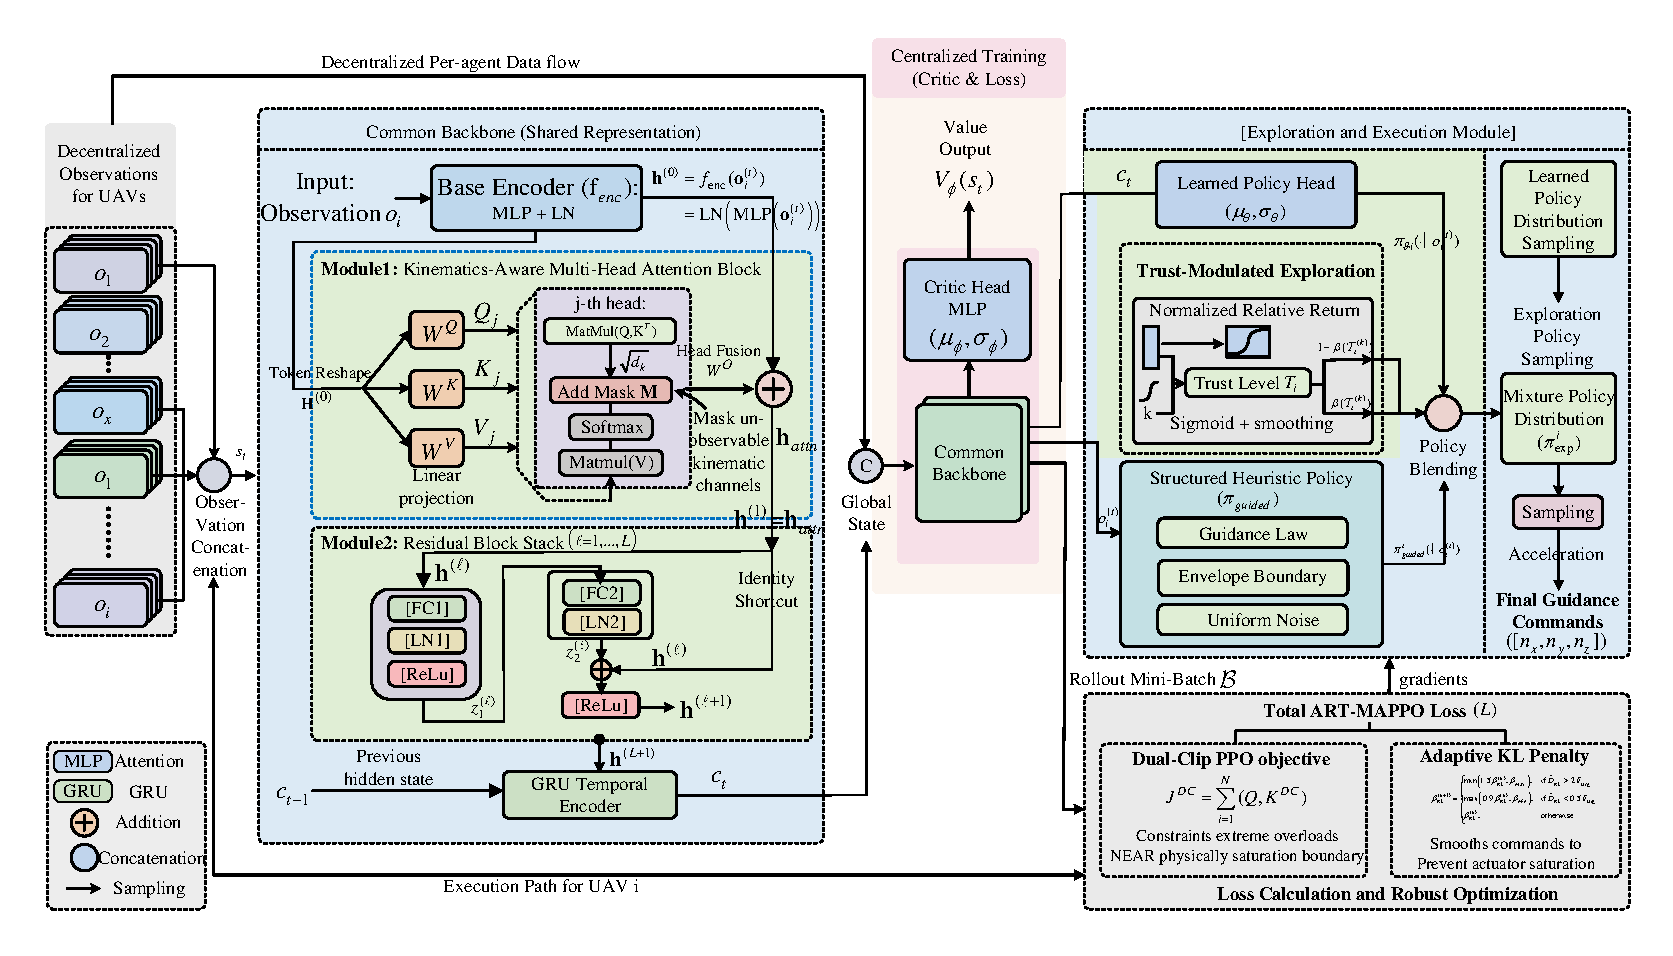
\includegraphics[width=7.3in]{rlsuanfa_3d.pdf}
\caption{Overall workflow of the ART-MAPPO algorithm for cooperative swarm interception, showing the interaction among the attention-residual network, trust-modulated exploration, dual-clip adaptive KL optimization, and the three-dimensional acceleration-command output.}
\label{fig:algorithm_flow}
\end{figure*}


\begin{algorithm}[!t]

\caption{ART-MAPPO for Cooperative Swarm Interception}
\label{alg:artmappo}
\begin{algorithmic}[1]

\REQUIRE Actor parameters $\{\boldsymbol{\vartheta}_i\}_{i=1}^{M}$;
centralized critic parameters $\phi$; episode horizon $T$;
training episodes $K$; PPO clip parameter $\epsilon$;
dual-clip floor $c$; target KL divergence $\delta_{\mathrm{targ}}$;
trust parameters $\alpha_T$, $\rho$, and $\tau_T$;
optimizer parameters

\ENSURE Trained decentralized policies
$\{\pi_{\boldsymbol{\vartheta}_i}\}_{i=1}^{M}$

\STATE Initialize $\{\boldsymbol{\vartheta}_i\}_{i=1}^{M}$ and $\phi$;
set $\mathcal{T}_i \leftarrow 0.5$ for each interceptor;
initialize $\beta_{\mathrm{KL}}$ and the running return statistics
$\mu_R$ and $\sigma_R^2$

\FOR{episode $k=1$ to $K$}

    \STATE Reset the environment, clear the rollout buffer,
    and reset $\mathbf{c}_{i,0}$ for each interceptor

    \STATE Set $\boldsymbol{\vartheta}_{i,\mathrm{old}} \leftarrow
    \boldsymbol{\vartheta}_i$ for all $i=1,\ldots,M$

    \STATE {\itshape // Decentralized rollout collection}

    \FOR{$t=0$ to $T-1$}

        \FOR{all interceptors $i=1,\ldots,M$ in parallel}

            \STATE Encode $\mathbf{o}_i^{(t)}$ using the
            attention--residual network according to
            \eqref{eq:encoder}--\eqref{eq:res_block_out},
            and update the temporal state $\mathbf{c}_{i,t}$
            using the GRU in \eqref{eq:gru}

            \STATE Form the policy
            $\pi_{\boldsymbol{\vartheta}_i}
            (\cdot\mid\mathbf{o}_i^{(t)})$
            according to \eqref{eq:actor_dist}, and sample
            $\mathbf{a}_{i,t}$ according to
            \eqref{eq:exploration_policy} and \eqref{eq:guided},
            with $\beta(\mathcal{T}_i)=1-\mathcal{T}_i$

            \STATE Clip $\mathbf{a}_{i,t}$ to the
            three-dimensional feasible action envelope $\mathcal{A}$

        \ENDFOR

        \STATE Step the environment once using the joint action
        $\mathbf{a}_t=
        (\mathbf{a}_{1,t},\ldots,\mathbf{a}_{M,t})$
        and store the joint transition in the rollout buffer

    \ENDFOR

    \STATE {\itshape // Trust update based on episode returns}

    \STATE Update $\mu_R$ and $\sigma_R^2$ using
    \eqref{eq:running_stats_mu} and
    \eqref{eq:running_stats_sigma}, and compute the normalized
    return $\widetilde{R}_i^{(k)}$ using
    \eqref{eq:trust_normalized}

    \STATE Update the trust level
    $\mathcal{T}_i^{(k+1)}$ using
    \eqref{eq:trust_evolution}

    \STATE {\itshape // Centralized optimization using the global state
    defined in \eqref{eq:critic_input}}

    \STATE Compute the GAE advantages $\hat{A}_t$ and value targets
    using \eqref{eq:gae_A} and \eqref{eq:gae_delta}

    \FOR{each mini-batch update}

        \STATE Evaluate the dual-clip surrogate objective
        $J^{\mathrm{DC}}(\boldsymbol{\vartheta})$ using
        \eqref{eq:standard_clip} and
        \eqref{eq:dual_clip_final}

        \STATE Estimate $\widehat{D}_{\mathrm{KL}}$ using
        \eqref{eq:kl_approx}, and compute the value loss
        $L_V(\phi)$ using \eqref{eq:value_loss}

        \STATE Update $\{\boldsymbol{\vartheta}_i\}_{i=1}^{M}$
        and $\phi$ by minimizing the total loss
        $\mathcal{L}(\boldsymbol{\vartheta},\phi)$ in
        \eqref{eq:total_loss} using AdamW with cosine
        learning-rate scheduling

    \ENDFOR

    \STATE Adapt the KL weight
    $\beta_{\mathrm{KL}}^{(k+1)}$ using
    \eqref{eq:kl_adapt}

\ENDFOR

\STATE \textbf{return}
$\{\pi_{\boldsymbol{\vartheta}_i}\}_{i=1}^{M}$

\end{algorithmic}
\end{algorithm}



%% -----------------------------------------------------------------------------------------

% \subsection{Theoretical Comparison with Conventional MAPPO Variants}}
% \label{subsec:theory_comparison}

% Having introduced the three modules, we now position ART-MAPPO against conventional
% MAPPO variants (standard MAPPO, IPPO, and single-clip PPO-penalty schemes) along the three
% axes most relevant to cooperative interception: convergence guarantees, the
% exploration--exploitation balance, and policy robustness. Table~\ref{tab:theory_comparison}
% summarizes the comparison, and each claim is traced to the governing equation.}

% \emph{1) Convergence guarantees.} In standard MAPPO the clipped surrogate
% \eqref{eq:standard_clip} is left-unbounded when $\hat{A}_t<0$: as $r_t(\theta)\!\to\!\infty$
% the term $r_t(\theta)\hat{A}_t\!\to\!-\infty$, so a single mini-batch with off-policy negative
% advantages can drive an arbitrarily large destructive update. In the interception setting these
% are exactly the aggressive terminal-overload samples, so the standard clip admits
% gradient explosions that manifest as the high inter-seed variance reported in
% Section~\ref{subsec:training}. The dual-clip objective \eqref{eq:dual_clip_final}
% floors the surrogate at $c\,\hat{A}_t$ and thereby confines the effective ratio to the compact
% set in \eqref{eq:rt_bound}, $r_t(\theta)\in[1/c,c]$. A per-step objective that is bounded on a
% compact ratio set has a Lipschitz-bounded policy gradient, so the stochastic update converges to
% an $\epsilon$-stationary point of the KL-penalized surrogate under the standard stochastic-approximation
% conditions for nonconvex objectives~\cite{ghadimi2013stochastic}; the bounded per-update policy shift
% that this surrogate enforces is precisely the trust-region principle whose monotonic-improvement bound
% motivates the design~\cite{schulman2015trust}, whereas conventional single-clip MAPPO leaves the ratio
% unbounded for $\hat{A}_t\!<\!0$ and forfeits this property. We claim convergence to a stationary point
% of the penalized surrogate rather than to a global optimum---the honest guarantee available to any
% PPO-family method---and this bounded-gradient behavior is the mechanism behind the $2\times$ smaller
% cross-seed standard deviation ($0.64$ vs.\ $1.34$) and the faster $90\%$-optimality crossing measured
% empirically.}

% \emph{2) Exploration--exploitation balance.} Conventional MAPPO regulates exploration
% with a \emph{fixed}, state-independent entropy bonus: every agent is pushed to explore by the
% same constant amount regardless of how well it is currently performing, and the exploration is
% undirected (isotropic noise on the action). ART-MAPPO instead makes the balance
% \emph{performance-adaptive and structured}. The trust recursion \eqref{eq:trust_evolution} is a
% contraction of modulus $(1-\alpha_T)$ toward the moving equilibrium
% $\mathcal{T}_i^{\star}=\sigma(\tau_T\tilde{R}_i)$, and the exploration weight
% $\beta(\mathcal{T}_i)=1-\mathcal{T}_i$ in \eqref{eq:exploration_policy} therefore shrinks for
% above-average performers and grows for below-average ones---at $\tilde{R}_i=\pm2$ the allocated
% exploration is $0.12$ versus $0.88$. Moreover the exploratory samples are drawn from the
% tactically informative mixture \eqref{eq:guided} (proportional-navigation exploitation, envelope
% probing, and residual coverage) rather than from undirected noise. The result is that
% exploration is spent where it is useful and withdrawn once a competent cooperative policy is
% found, which explains the smooth, monotone entropy decay observed for ART-MAPPO against the
% flatter entropy profile of standard MAPPO.}

% \emph{3) Policy robustness.} Standard MAPPO controls inter-update policy drift with a
% \emph{single, fixed} mechanism---either a constant clip $\epsilon$ or a constant KL weight. No
% single fixed penalty is uniformly adequate: a small weight lets $\hat{D}_{\mathrm{KL}}$ spike far
% outside the trust region during aggressive-exploration bursts (risking the load-factor excursions
% of Section~\ref{subsec:dual_clip_kl}), while a large weight over-regularizes during calm phases
% and stalls terminal-guidance refinement. The adaptive-KL controller \eqref{eq:kl_adapt} closes a
% feedback loop around the target $\delta_{\mathrm{targ}}$, multiplicatively increasing
% $\beta_{\mathrm{KL}}$ when $\hat{D}_{\mathrm{KL}}>2\delta_{\mathrm{targ}}$ and relaxing it when
% $\hat{D}_{\mathrm{KL}}<0.5\delta_{\mathrm{targ}}$, so the realized policy shift is confined to a
% bounded band across both regimes. Coupled with the two-sided ratio bound \eqref{eq:rt_bound}, this
% gives ART-MAPPO a bounded, self-correcting response to the noisy, delayed observations of the
% interception environment---the robustness that the Monte Carlo and hardware-in-the-loop studies
% in Section~\ref{sec:simulation} confirm in closed loop. A quantitative illustration of all three
% mechanisms, computed directly from Eqs.~\eqref{eq:dual_clip_final}, \eqref{eq:trust_evolution},
% and \eqref{eq:kl_adapt}, is provided in the supplementary response material.}

% \begin{table}[!t]
% 
% \centering
% \caption{Theoretical comparison of ART-MAPPO with conventional MAPPO variants.}}
% \label{tab:theory_comparison}
% \renewcommand{\arraystretch}{1.25}
% \resizebox{\columnwidth}{!}{%
% \begin{tabular}{@{}p{2.05cm}p{2.75cm}p{2.95cm}@{}}
% \toprule
% \textbf{Axis} & \textbf{Conventional MAPPO} & \textbf{ART-MAPPO (this work)} \\
% \midrule
% Convergence guarantee &
% Single clip \eqref{eq:standard_clip} unbounded for $\hat{A}_t<0$; large destructive updates possible &
% Dual-clip \eqref{eq:dual_clip_final} floors objective, ratio confined to $[1/c,c]$ \eqref{eq:rt_bound}; bounded gradients \\
% Exploration vs.\ exploitation &
% Fixed entropy bonus; undirected, performance-independent &
% Trust-modulated \eqref{eq:trust_evolution}, \eqref{eq:exploration_policy}; performance-adaptive, tactically structured \eqref{eq:guided} \\
% Policy robustness &
% Fixed penalty; drift not uniformly bounded across regimes &
% Adaptive-KL feedback \eqref{eq:kl_adapt} confines $\hat{D}_{\mathrm{KL}}$ to a band around $\delta_{\mathrm{targ}}$ \\
% Empirical effect &
% Cross-seed $\sigma=1.34$; $90\%$ opt.\ at ep.\ $7654$ &
% Cross-seed $\sigma=0.64$; $90\%$ opt.\ at ep.\ $5591$; $+12.3\%$ reward \\
% \bottomrule
% \end{tabular}%
% }
% \end{table}
%% -----------------------------------------------------------------------------------------


% \subsection{Mechanistic Comparison with Conventional MAPPO Variants}}
% \label{subsec:theory_comparison}

% Having introduced the main components of ART-MAPPO, this subsection compares the proposed framework with conventional MAPPO variants from three perspectives that are particularly relevant to cooperative interception: convergence-related optimization behavior, the exploration--exploitation balance, and policy-update robustness. Standard MAPPO and IPPO mainly differ in the information available to the critic, whereas their actor-side PPO clipping and entropy-regularized exploration mechanisms are generally similar. They are therefore discussed together when comparing these actor-side properties. Fixed-penalty PPO variants are also considered because they regulate policy changes using a constant KL coefficient rather than the feedback-adjusted regularization adopted in ART-MAPPO.}

% \emph{1) Convergence-related optimization behavior.}
% Because the policy and value functions are represented by deep neural networks, neither conventional MAPPO nor ART-MAPPO generally provides a guarantee of convergence to a global optimum. The relevant distinction is therefore not a stronger global convergence theorem, but the manner in which the policy-update objective suppresses excessively large and potentially destructive stochastic updates. For the conventional PPO clipped surrogate in \eqref{eq:standard_clip}, when $\hat{A}_t<0$ and the probability ratio $r_t(\theta)$ becomes sufficiently large, the term $r_t(\theta)\hat{A}_t$ may produce an increasingly negative surrogate contribution. Consequently, a small number of large-ratio negative-advantage samples may exert a disproportionately strong influence on a mini-batch update. In the considered interception problem, such samples may arise from aggressive guidance actions that increase terminal overload, miss distance, or temporal-coordination error.}

% The dual-clip objective in \eqref{eq:dual_clip_final} introduces the additional term $c\hat{A}_t$ for negative-advantage samples. Once the corresponding surrogate contribution becomes more negative than this threshold, it is saturated rather than allowed to decrease indefinitely. Thus, Dual-Clip limits the effective contribution of large-ratio negative-advantage samples to the policy-gradient update. This statement concerns the surrogate contribution and does not imply that the actual probability ratio of every sample is subject to an additional hard interval constraint. The adaptive KL penalty further discourages an excessive average deviation between successive policies. Together, these mechanisms reduce sensitivity to abnormal mini-batches and high-variance advantage estimates, thereby promoting a more controlled optimization process. They follow the trust-region motivation of restricting abrupt policy changes~\cite{schulman2015trust}, but should be interpreted as update-stabilization mechanisms rather than as a formal guarantee of monotonic improvement or global convergence.}

% \emph{2) Exploration--exploitation balance.}
% Conventional MAPPO commonly maintains exploration through an entropy bonus with a fixed coefficient. Although entropy regularization prevents the policy from becoming deterministic too early, its exploration strength is not explicitly adjusted according to the relative performance of individual agents. Moreover, the entropy term itself does not specify which exploratory actions are tactically meaningful for cooperative interception. Consequently, agents that have already learned effective guidance behavior and agents that remain trapped in inferior strategies may receive similar exploration incentives.}

% ART-MAPPO instead employs the trust-modulated mechanism in \eqref{eq:trust_evolution} and \eqref{eq:exploration_policy}. For a fixed normalized return, the trust recursion moves the current trust value toward a performance-dependent target. During training, it acts as an exponentially smoothed tracker of the relative performance of each agent. An agent whose recent return exceeds the swarm average gradually assigns greater weight to its learned policy, whereas a below-average agent retains a larger exploratory component. The amount of exploration is therefore adjusted according to the learning status of each agent rather than being uniformly prescribed.}

% In addition, the exploratory component is drawn from the task-informed mixture in \eqref{eq:guided}, which combines policy-preferred actions, flight-envelope probing actions, and residual action-space coverage. The proposed mechanism therefore regulates both the intensity and the structure of exploration. It promotes broad strategy discovery during the early training stage while progressively emphasizing exploitation after an effective cooperative policy has emerged. Compared with the fixed entropy mechanism used in conventional MAPPO, this performance-adaptive exploration strategy allocates additional exploration to agents whose policies remain inadequate and reduces unnecessary perturbations for agents that have already acquired effective cooperative behavior. The entropy reduction and reward improvement reported in Section~\ref{subsec:training} are consistent with this intended transition from exploration to exploitation.}

% \emph{3) Policy-update robustness.}
% Conventional MAPPO normally regulates policy updates using a fixed clipping threshold. PPO-penalty variants may additionally employ a constant KL penalty coefficient. However, a fixed regularization strength may not be equally suitable throughout the complete training process. A weak penalty may permit an excessive policy shift during aggressive exploratory updates, whereas an overly strong penalty may unnecessarily suppress policy refinement after the strategy has entered a comparatively stable region.}

% The adaptive KL mechanism in \eqref{eq:kl_adapt} introduces feedback regulation based on the empirical KL divergence between successive policies. When $\hat{D}_{\mathrm{KL}}$ exceeds the prescribed target range, the KL coefficient is increased so that subsequent policy changes receive a stronger penalty. When the observed divergence remains substantially below the target, the coefficient is reduced to permit further policy refinement. The adaptive mechanism does not impose a strict hard bound on the KL divergence in every update; instead, it continually steers the average policy deviation toward the desired operating range.}

% When combined with the Dual-Clip safeguard, adaptive KL regularization reduces the sensitivity of policy optimization to noisy mini-batches, delayed advantage estimates, and occasional large-ratio negative-advantage samples. In this subsection, policy robustness primarily refers to the numerical stability of policy optimization and the suppression of abrupt inter-update policy changes. Robustness to sensor noise, communication delay, target maneuver uncertainty, and model mismatch remains a closed-loop property of the complete guidance framework rather than a direct theoretical consequence of the KL controller alone. The Monte Carlo and hardware-in-the-loop experiments in Section~\ref{sec:simulation} evaluate this system-level robustness empirically, whereas the present discussion explains the optimization mechanisms that contribute to the observed performance.}

% In summary, ART-MAPPO does not claim a stronger formal global-convergence guarantee than conventional MAPPO variants. Its distinction lies in three complementary mechanisms. Dual-Clip limits the excessive influence of unfavorable large-ratio samples, trust-modulated exploration allocates structured exploration according to agent performance, and adaptive KL regularization adjusts the regularization strength according to the realized policy deviation. These mechanisms respectively improve the controllability of stochastic policy updates, the efficiency of cooperative-strategy exploration, and the adaptability of policy regularization across different training stages. The training results in Section~\ref{subsec:training} and the closed-loop evaluations in Section~\ref{sec:simulation} provide empirical evidence for the associated improvements in learning efficiency, optimization stability, and cooperative interception performance.}


\subsection{Mechanistic Comparison with Conventional MAPPO}
\label{subsec:theory_comparison}

\emph{1) Convergence analysis.}
Conventional MAPPO primarily relies on centralized value estimation, GAE, and
a fixed clipped surrogate to support policy learning. In ART-MAPPO, the
attention--residual encoder preserves the coupled kinematic information and
maintains a direct gradient path, while the GRU incorporates maneuver history
into the policy representation. This reduces the sensitivity of policy learning
to instantaneous state variations. The smoothed trust variable changes the
guided-exploration weight gradually according to relative return, allowing the
sampling policy to shift steadily toward exploitation as effective cooperative
behavior develops. During parameter optimization, Dual-Clip limits anomalous
negative surrogate contributions, and adaptive KL regularization adjusts the
penalty according to the observed policy deviation. The resulting learning
process exhibits lower sampling and update variability, promoting a more stable
approach to the steady training regime than conventional MAPPO.

% \emph{2) Exploration--exploitation balance.}
% Conventional MAPPO primarily maintains exploration through an entropy bonus
% with a fixed coefficient, whose strength is not explicitly adjusted according
% to agent-specific performance. ART-MAPPO retains this entropy regularization
% and additionally introduces the trust-modulated mechanism in
% \eqref{eq:trust_evolution}--\eqref{eq:exploration_policy}. Agents with higher
% relative returns place greater weight on their learned policies, whereas agents
% with lower relative returns retain a larger task-informed exploratory
% component. ART-MAPPO therefore adjusts exploration according to the relative
% learning performance of individual agents instead of relying solely on a
% uniform exploration incentive.}

\emph{2) Exploration--exploitation balance.}
In the conventional MAPPO baseline adopted in this study, stochastic action
sampling and a fixed-coefficient entropy bonus provide an exploration incentive
that is not explicitly conditioned on agent-specific performance. ART-MAPPO
retains entropy regularization and additionally introduces the trust-modulated
mechanism in \eqref{eq:trust_evolution}--\eqref{eq:exploration_policy}. For a
fixed normalized return, the trust recursion is a contraction toward a
performance-dependent target; during training, it acts as a bounded,
exponentially smoothed tracker of relative agent performance. Agents that
persistently achieve above-average returns are gradually assigned greater
weight to their learned policies, whereas below-average agents retain a larger
task-informed policy component. ART-MAPPO therefore adapts the intensity and
structure of exploration across agents, rather than relying solely on a uniform
entropy incentive. 

\emph{3) Policy robustness.}
The fixed clipping mechanism of conventional MAPPO cannot adjust its
regularization strength according to the policy deviation realized during
training. In ART-MAPPO, the adaptive KL mechanism strengthens the penalty when
the empirical KL divergence is excessive and relaxes it when the divergence
remains below the target range. Combined with Dual-Clip, this feedback reduces
the sensitivity of policy optimization to abnormal mini-batches and abrupt
inter-update changes. 

% 意见回复要写上这段话，这里只是理论分析，实验分析在XXX章节。 Here, policy robustness refers to the numerical stability of policy updates, while robustness of the complete guidance policy to target maneuvers, sensing uncertainty, and communication delay is evaluated empirically in Section~ ef{sec:simulation}.}


\subsection{State Representation and Reward Design}
\label{subsec:state_reward}

\emph{1) Observation Space:} The observation vector for interceptor $i$ at time step $t$ is designed to capture the essential kinematic quantities for guidance and coordination:
\begin{equation}
\label{eq:observation_space}
\begin{aligned}
\mathbf{o}_i^{(t)}={}&\bigl[o_i^{(t),1},\;o_i^{(t),2},\;o_i^{(t),3},\\[-2pt]
&\quad o_i^{(t),4},\;o_i^{(t),5},\;o_i^{(t),6}\bigr]^\top\in\mathbb{R}^{n_o},\quad n_o=6
\end{aligned}
\end{equation}
The six components are defined as:
\begin{equation}
\label{eq:o1}
o_i^{(t),1} =
\begin{cases}
\dfrac{V_i \dot{q}_i^{\gamma}(t)}{g}, &
\left|\dot{q}_i^{\gamma}(t) - \dot{q}_i^{\gamma}(t-1)\right|
\leq \Delta \dot{q}_{\max}
\\[0pt]
\dfrac{V_i \dot{q}_i^{\gamma}(t-1)}{g}, &
\left|\dot{q}_i^{\gamma}(t) - \dot{q}_i^{\gamma}(t-1)\right|
> \Delta \dot{q}_{\max}
\end{cases}
\end{equation}

\begin{equation}
\label{eq:o2}
o_i^{(t),2} = \gamma_i-q_i^{\gamma}
\end{equation}

\begin{equation}
\label{eq:o3}
o_i^{(t),3} =
\begin{cases}
\dfrac{V_i \dot{q}_i^{\theta}(t)}{g}, &
\left|\dot{q}_i^{\theta}(t) - \dot{q}_i^{\theta}(t-1)\right|
\leq \Delta \dot{q}_{\max}
\\[0pt]
\dfrac{V_i \dot{q}_i^{\theta}(t-1)}{g}, &
\left|\dot{q}_i^{\theta}(t) - \dot{q}_i^{\theta}(t-1)\right|
> \Delta \dot{q}_{\max}
\end{cases}
\end{equation}

\begin{equation}
\label{eq:o4}
o_i^{(t),4} = \theta_i-q_i^{\theta}
\end{equation}

\begin{equation}
\label{eq:o5}
o_i^{(t),5}
=
\left(n_{x_i}^2+n_{y_i}^2+n_{z_i}^2\right)\Delta t
\end{equation}

\begin{equation}
\label{eq:o6}
o_i^{(t),6}
=
\frac{r_i}{\min_{j\in\mathcal{G}_i}t_{go_j}}-V_i
\end{equation}
where $\Delta\dot{q}_{\max}=0.03$~rad/s is the LOS-rate noise threshold, $\mathcal{G}_i$ denotes the set of interceptors assigned to the same target as interceptor $i$, and $\Delta t$ is the simulation timestep. 
Component $o_i^{(t),1}$ is a smoothed lateral acceleration proportional to $V_i\dot q_i^{\gamma}/g$, where the previous LOS-rate estimate is retained when the instantaneous measurement jump exceeds $\Delta\dot q_{\max}$.
Component $o_i^{(t),2}$ is the horizontal lead-angle deviation $\gamma_i-q_i^{\gamma}$.
Components $o_i^{(t),3}$ and $o_i^{(t),4}$ are the corresponding vertical-plane features, proportional to $V_i\dot q_i^{\theta}/g$ and $\theta_i-q_i^{\theta}$. Here, $q_i^{\gamma}$ and $q_i^{\theta}$ denote the LOS azimuth and elevation angles from interceptor $i$ to its assigned target.
Component $o_i^{(t),5}$ encodes the three-dimensional control effort, and component $o_i^{(t),6}$ is the velocity error relative to the desired approach speed $r_i/\min_j t_{go_j}$, which drives time-coordinated impact.



\emph{2) Reward Function:} The reward function incorporates five components to guide the learning process:
\begin{equation}
\label{eq:reward_function}
\begin{split}
r_i^{(t)} =& \; w_1 r_i^{\text{dist}} + w_2 r_i^{\text{angle}} + w_3 r_i^{\text{hit}} \\
&+ w_4 r_i^{\text{coord}} + w_5 r_i^{\text{energy}}
\end{split}
\end{equation}
with each component defined as:
\begin{align}
r_i^{\text{dist}} &= \exp\!\left(-\alpha_d \left\|\mathbf{p}_i^{(t)} - \mathbf{p}_{\text{tgt}}\right\|\right) \label{eq:r_dist}\\
r_i^{\text{angle}} &= -\alpha_a\sqrt{\left(\gamma_i-q_i^{\gamma}\right)^2+\left(\theta_i-q_i^{\theta}\right)^2} \label{eq:r_angle}\\
r_i^{\text{hit}} &= R_{\text{hit}} \cdot \mathbb{I}\!\left(\left\|\mathbf{p}_i^{(t)} - \mathbf{p}_{\text{tgt}}\right\| < d_{\text{kill}}\right) \label{eq:r_hit}\\
r_i^{\text{coord}} &= -\alpha_c \left| t_{go_i}^{(t)} - \bar{t}_{go}^{(t)} \right|, \quad \bar{t}_{go}^{(t)} = \frac{1}{|\mathcal{G}_i|}\sum_{j \in \mathcal{G}_i} t_{go_j}^{(t)} \label{eq:r_coord}\\
r_i^{\text{energy}} &= -\alpha_e\left(n_{x_i}^2+n_{y_i}^2+n_{z_i}^2\right) \label{eq:r_energy}
\end{align}
where $\mathbf{p}_i^{(t)}=[x_i,y_i,z_i]^\top$ and $\mathbf{p}_{\mathrm{tgt}}=[x_{\mathrm{tgt}},y_{\mathrm{tgt}},z_{\mathrm{tgt}}]^\top$ are the interceptor and target positions, $d_{\text{kill}}$ is the lethal radius, $R_{\text{hit}} > 0$ is the terminal success reward, and $w_k$, $\alpha_k$ are weighting coefficients. The distance reward $r_i^{\text{dist}} \in (0,1]$ provides dense, bounded feedback for target approach. 
The coordination reward $r_i^{\text{coord}}$ penalizes deviation from the group mean time-to-go $\bar{t}_{go}^{(t)}$, encouraging simultaneous interception.
The energy term $r_i^{\text{energy}}$ regularizes control effort to prevent actuator saturation.

Each weight $w_k$ emphasizes one tactical dimension: $w_1$ shapes the dense approach signal, $w_2$ aligns the three-dimensional terminal geometry, $w_3$ rewards the terminal hit, $w_4$ promotes impact-time coordination, and $w_5$ penalizes control effort. The sensitivity of $w_1$--$w_5$ is analyzed in Section~\ref{subsec:parameter_sensitivity}.

\subsection{Evaluation Criteria}
\label{subsec:eval}

To quantitatively evaluate the proposed cooperative interception method, we adopt four metrics that capture temporal coordination, terminal lateral-acceleration safety, guidance accuracy, and operational efficiency. The first three metrics are formally defined as follows.
\begin{equation}
\label{E1}
E_{co\text{-}time} = \frac{1}{m}\sum_{i=1}^{m} \left| t_{go_i} - \frac{1}{m}\sum_{j=1}^{m} t_{go_j} \right|
\end{equation}
\begin{equation}
\label{E2}
E_{n} = \frac{1}{m}\sum_{i=1}^{m} |n_{y_i}|
\end{equation}
\begin{equation}
\label{E3}
E_{miss} = \frac{1}{m}\sum_{i=1}^{m} d_{tf_i}
\end{equation}

Here, Eq.~\eqref{E1} measures the mean deviation of individual time-to-go values from the group mean, thereby assessing temporal coordination among interceptors assigned to the same target. Eq.~\eqref{E2} gives the average terminal lateral acceleration, which reflects control effort and maneuver aggressiveness during the terminal guidance phase. Eq.~\eqref{E3} denotes the mean terminal miss distance, where $d_{tf_i}$ is the relative distance between interceptor $i$ and its assigned target at the terminal engagement time $t_{f_i}$, serving as a direct indicator of guidance accuracy. The fourth metric, coordinated interception duration, quantifies operational efficiency. All four metrics are reported in the simulation results to provide a comprehensive assessment of effectiveness, safety, precision, and efficiency.










%% ===========================================================
\section{Simulation Verification}
\label{sec:simulation}

\subsection{Experimental Setup and Implementation Details}
\label{subsec:setup}

All training and evaluation were performed on an Intel Core i7-9700F CPU / Nvidia RTX 3090
GPU server running Ubuntu 18.04.
The simulation step size was 50\,ms.
Table~\ref{table2} summarizes the key hyperparameters of ART-MAPPO.

\begin{table}[t]
\centering
\renewcommand{\arraystretch}{1.4}
\caption{ART-MAPPO Algorithm Parameters}
\label{table2}
\begin{tabular}{ll}
\hline\hline
Parameter & Value \\ \hline
PPO clipping factor ($\epsilon$) & 0.2 \\
Dual-clip parameter ($c$) & 3.0 \\
Target KL divergence ($\delta_{\text{targ}}$) & 0.02 \\
Entropy bonus coefficient ($c_e$) & 0.01 \\
GAE parameter ($\lambda_{\mathrm{GAE}}$) & 0.97 \\
Discount factor ($\gamma_{\mathrm{RL}}$) & 0.99 \\
LR schedule & Cosine Annealing \\
Optimizer & AdamW \\
Mini-batch number & 4 \\
Buffer size & 4096 \\
Learning rate & $3\times10^{-4}$ \\
Attention heads ($H$) & 4 \\
Residual blocks ($L$) & 2 \\ \hline
\end{tabular}
\end{table}


The simulation environment is depicted in Fig.~\ref{chushi}.
$A_{\text{UAV}}$ are randomly spawned within an annular region of radii $D_1$--$D_2$\,m with speed
$V_A\in[10,40]$\,m/s. To simulate a directional swarm attack toward the high-value target area, their initial heading angles $\gamma_A$ are uniformly distributed within $[q_A^{\gamma}-\pi/6,q_A^{\gamma}+\pi/6]$, where $q_A^{\gamma}$ denotes the initial LOS azimuth angle from the specific attacker to the center of the defended area.
$D_{\text{UAV}}$ are uniformly distributed within a disk of radius $D_3$\,m with
$V_D\in[10,40]$\,m/s and $\gamma_D\in[0,2\pi]$.
The initial altitudes are $z_A=120$~m and $z_D=0$~m, and the initial flight-path angles are $\theta_A=\theta_D=0$.


\begin{figure}[!t]
\centering
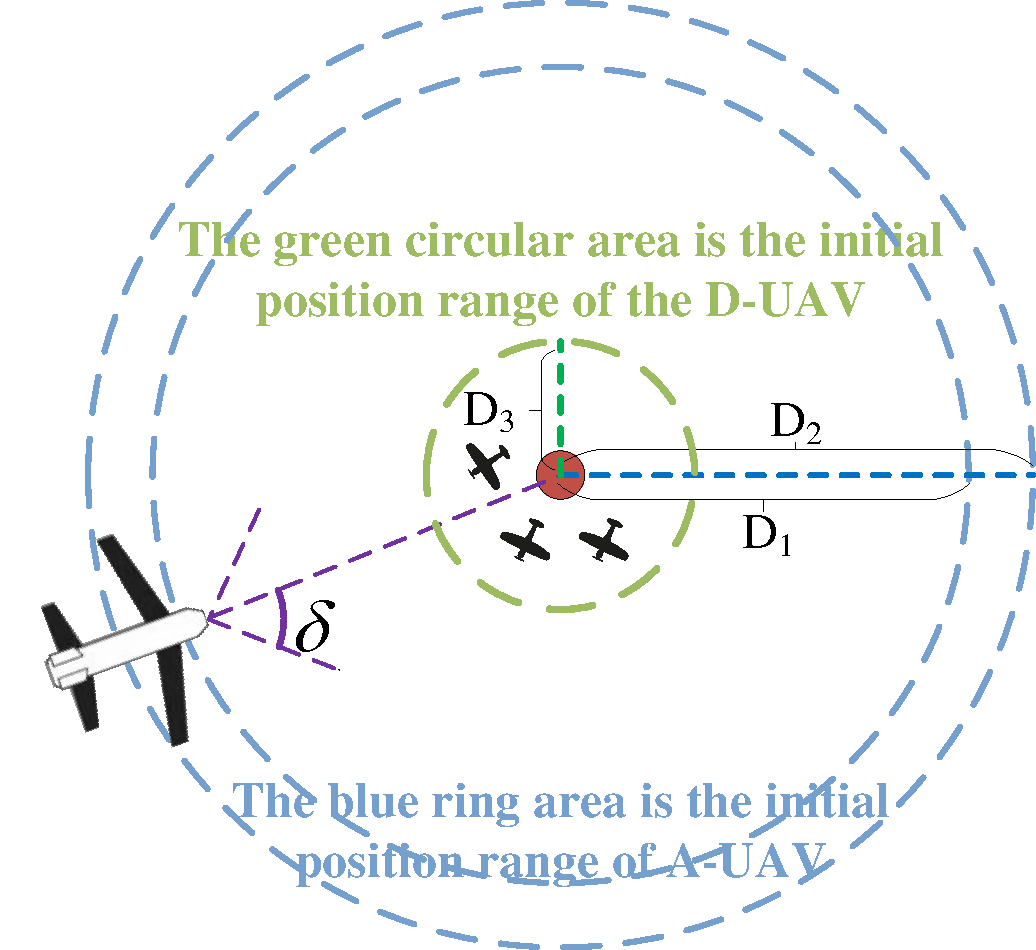
\includegraphics[width=3.0in]{chushi01.pdf}
\caption{Simulation environment configuration for training.}
\label{chushi}
\end{figure}

A representative scenario of 20 $D_{\text{UAV}}$ versus 8 $A_{\text{UAV}}$ is considered, with $D_1=1500$\,m,
$D_2=1600$\,m, and $D_3=100$\,m.
The initial horizontal position is specified by the radial coordinate $r$ and polar angle $\varphi$ about the defended-area center.
Table~\ref{chushicanshu} summarizes the UAV kinematic parameters.

\begin{table*}[!t]
\centering
\caption{UAV Parameters for Attackers and Defenders}
\label{chushicanshu}
\renewcommand{\arraystretch}{1.6}
\footnotesize
\setlength{\tabcolsep}{3pt}
\begin{tabular}{ccccc}
\hline\hline
 & Initial position $(r,\varphi,z)$ & Initial velocity $V$ & \shortstack{Initial heading angle $\gamma$\\ Initial flight-path angle $\theta$} & \shortstack{Maneuverability\\ $(n_x,n_y,n_z)$} \\ \hline
$D_{\text{UAV}}$ & \shortstack{$r\sim U[0,D_3]$, $\varphi_D\sim U[0,2\pi)$\\ $z_D=0$\,m} & $V_D\sim U[10,40]$\,m/s & \shortstack{$\gamma_D\sim U[0,2\pi]$\\ $\theta_D=0$} & \shortstack{$n_x\in[-0.1g,1g]$, $n_y\in[-1g,1g]$\\ $n_z\in[-1g,1g]$} \\
$A_{\text{UAV}}$ & \shortstack{$r\sim U[D_1,D_2]$, $\varphi_A\sim U[0,2\pi)$\\ $z_A=120$\,m} & $V_A\sim U[10,40]$\,m/s & \shortstack{$\gamma_A\sim U[q_A^{\gamma}-\pi/6,q_A^{\gamma}+\pi/6]$\\ $\theta_A=0$} & \shortstack{$n_x=0$, $n_y\in[-1g,1g]$\\ $n_z\in[-1g,1g]$} \\ \hline
\end{tabular}
\end{table*}

Two dynamic engagement scenarios are designed to evaluate cooperative guidance performance.
A third scenario, is used in Section~\ref{subsec:montecarlo} to provide additional validation of the proposed method under an unseen bang--bang attack pattern.
The scenario configurations are listed in Table~\ref{changjingqingkuang}.


\begin{table}[!t]
\centering
\renewcommand{\arraystretch}{1.4}
\caption{Combat Scenario Settings}
\label{changjingqingkuang}
\begin{tabular}{cccc}
\hline\hline
 & $N_{D\text{-UAV}}$ & $N_{A\text{-UAV}}$ & $A_{\text{UAV}}$ Strategy \\ \hline
Case 1 & 20 & 8 & Hybrid Evasion \\
Case 2 & 20 & 8 & Sinusoidal Maneuver \\
Case 3 & 20 & 8 & Bang-Bang Evasion \\ \hline
\end{tabular}
\end{table}


The hardware-in-the-loop (HIL) experimental environment is configured as follows.
\emph{1) Communication Delay and Sensing Uncertainty:}
Communication and sensing nonidealities are incorporated into the
three-dimensional simulation. The position and velocity measurements used to
construct the defender observations are delayed and corrupted by independent
zero-mean Gaussian noise,
\begin{equation}
\label{eq:noise_model}
{
\widehat{\mathbf{p}}(t)
=
\mathbf{p}(t-\tau_s)+\boldsymbol{\eta}_p,
\qquad
\widehat{\mathbf{v}}(t)
=
\mathbf{v}(t-\tau_s)+\boldsymbol{\eta}_v,}
\end{equation}
where
$\boldsymbol{\eta}_p\sim\mathcal{N}(\mathbf{0},\sigma_p^2\mathbf{I}_3)$
and
$\boldsymbol{\eta}_v\sim\mathcal{N}(\mathbf{0},\sigma_v^2\mathbf{I}_3)$.
The nominal settings are
$\tau_s=50$~ms,
$\sigma_p=1$~m, and
$\sigma_v=0.3$~m/s.
All derived observation variables, including the LOS geometry, closing speed,
and time-to-go, are recomputed from the delayed noisy Cartesian states.
The communication process is subject to a $50$~ms communication delay and 
a $1\%$ packet-loss rate, with the latest valid state packet retained 
when a packet is lost.
\emph{2) HIL Platform:}
As shown in Fig.~\ref{fig:hil_platform}, the three-dimensional interception experiment is further implemented on a
HIL platform. The policies of defenders $D_0$--$D_4$ are
deployed on five independent NVIDIA Jetson NX computers, with one defender
assigned to each node. The corresponding target-assignment algorithm is also
executed on the Jetson NX nodes. The engagement dynamics, attacker cluster,
and software policies of the remaining defenders $D_5$--$D_n$ are executed on
the simulation server. The server and Jetson NX nodes exchange observations,
actions, and target-assignment results through a physical TCP Ethernet network
under the communication conditions described above.

\begin{figure}[!t]
\centering
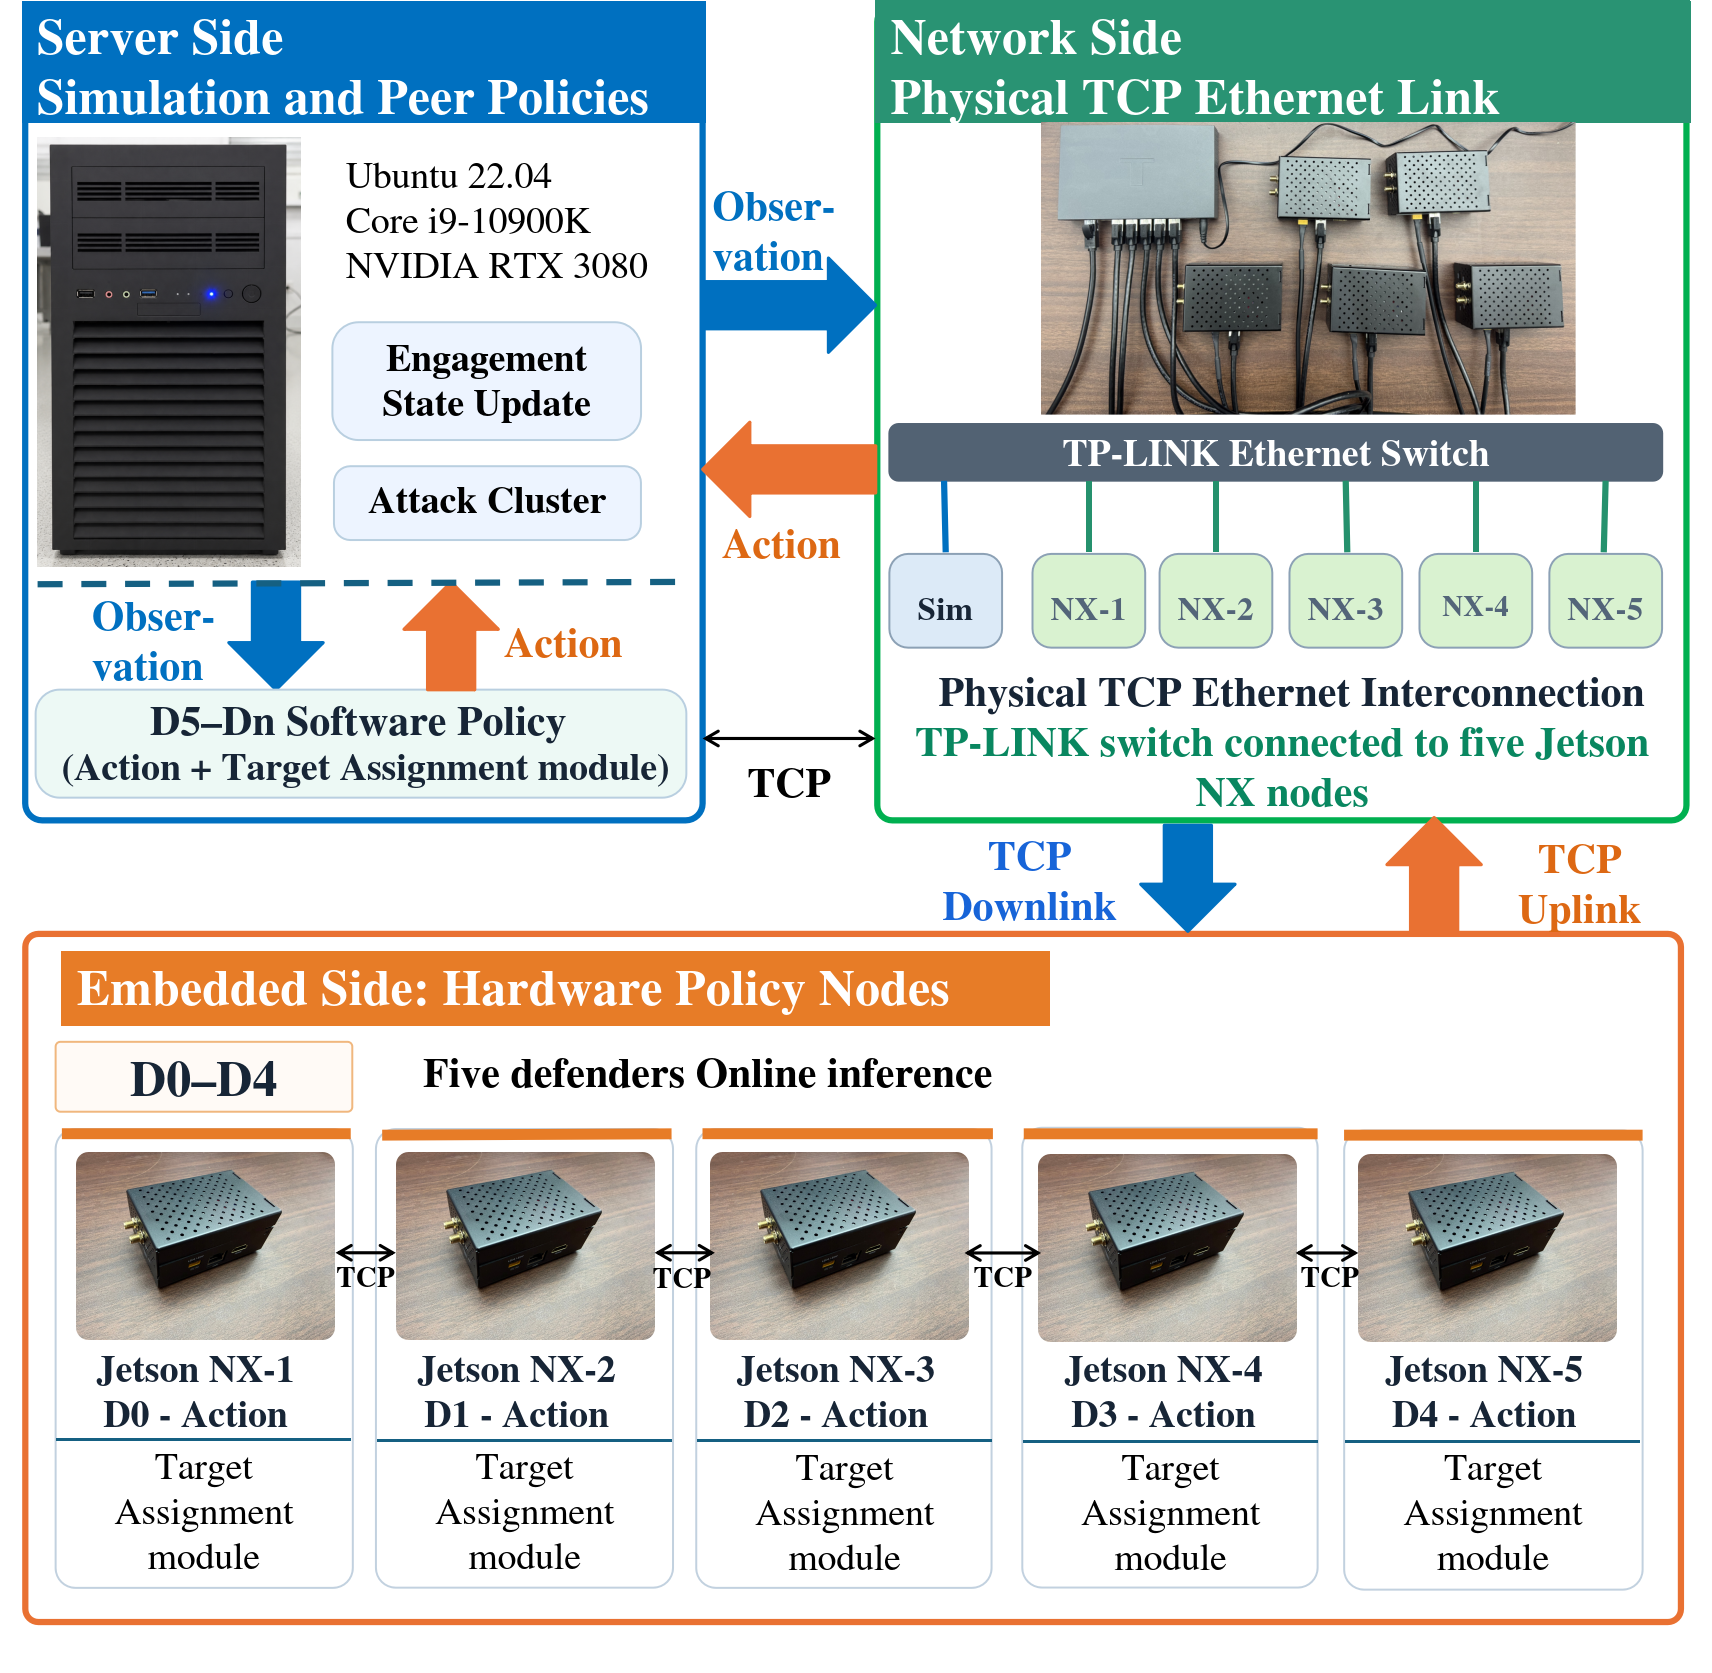
\includegraphics[width=0.48\textwidth]{TASE_HIL.png}
\caption{HIL platform.}
\label{fig:hil_platform}
\end{figure}




\subsection{Target Assignment Performance and Spatial Topology}
\label{subsec:assignment_results}

To evaluate the IDBO algorithm, it is benchmarked against PSO, GWO, SSA, BOA, and standard DBO in case 1. 

Fig.~\ref{fig:convergence} illustrates the statistical performance in terms of average cost convergence over iterations. IDBO significantly outperforms the baselines, reaching the lowest steady-state cost within 100~iterations. 
\begin{figure}[!ht] 
\centering 
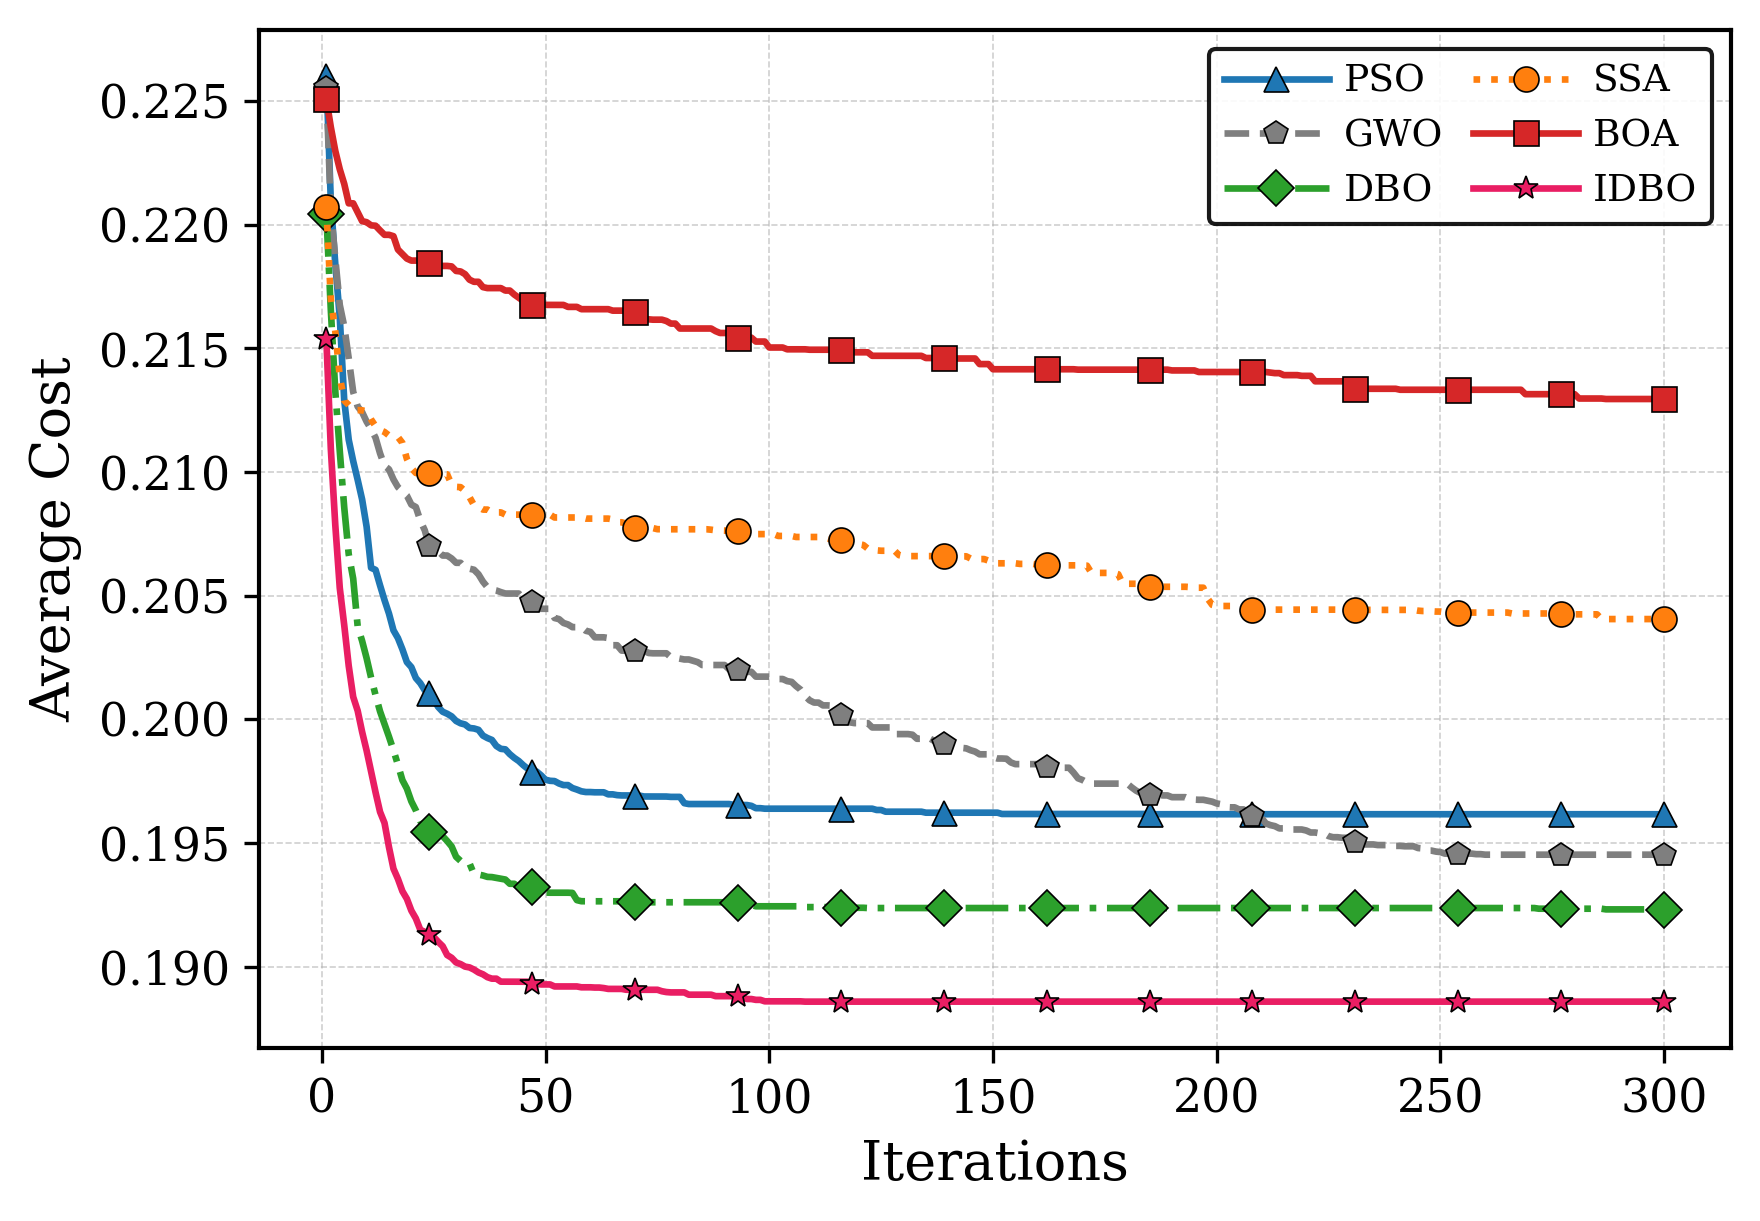
\includegraphics[width=3.25in]{convergence.png} 
\caption{Average cost convergence over iterations for target assignment algorithms.} 
\label{fig:convergence} 
\end{figure}

Furthermore, the violin plot in Fig.~\ref{fig:violin} evaluates the algorithmic robustness across multiple independent runs. It shows IDBO's compact distribution at the lowest median cost, highlighting its superior stability and consistency compared to the other heuristic methods.

\begin{figure}[!ht] 
\centering 
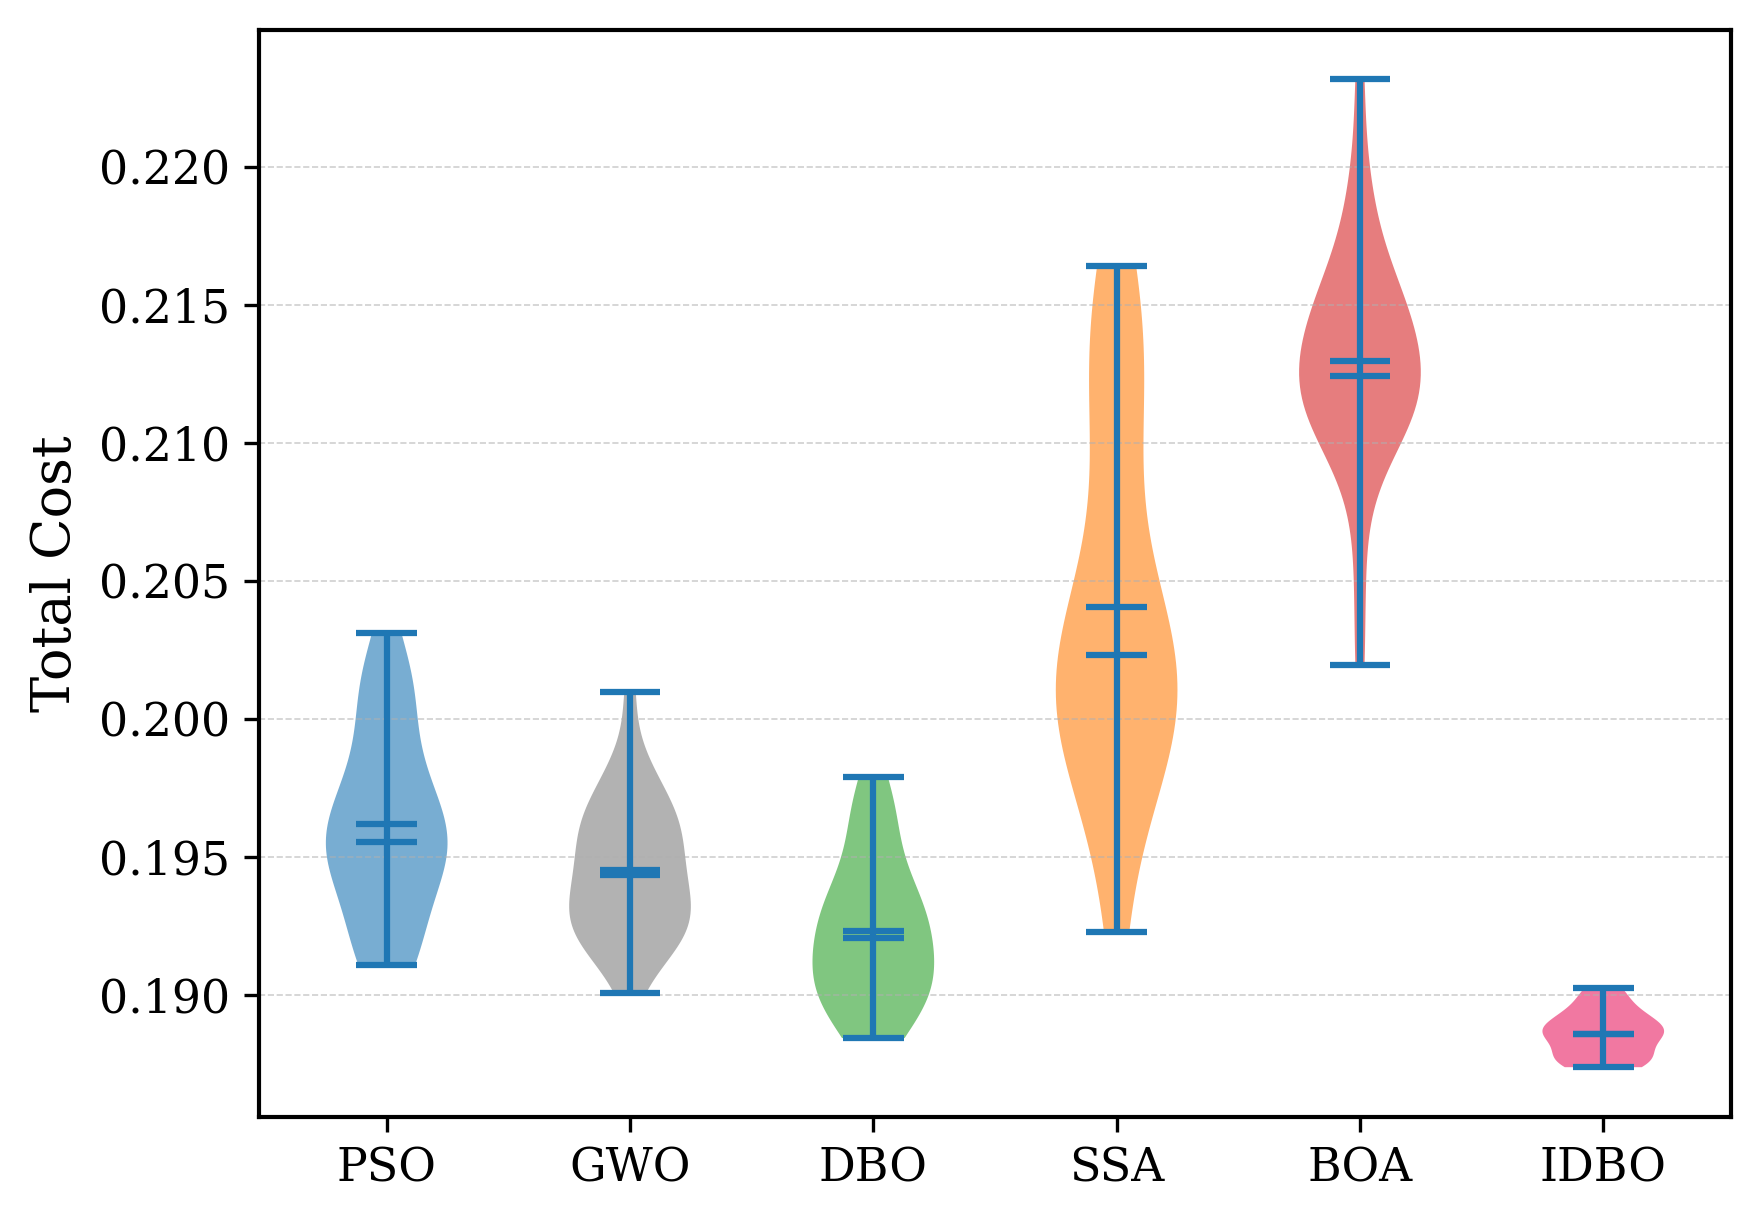
\includegraphics[width=3.2in]{violin.png} 
\caption{Violin plot of total cost distribution evaluating algorithm robustness.} 
\label{fig:violin} 
\end{figure}

The optimal assignment mapping generated by the algorithm is visualized in Fig.~\ref{fig:assignment_topology}. Attackers $A_1$--$A_4$ are each allocated three defenders, while $A_5$--$A_8$ are intercepted by two defenders each, perfectly respecting the per-target capacity constraint $L_{\max}$ and ensuring sufficient numerical superiority for cooperative strikes.

\begin{figure}[!ht]
\centering
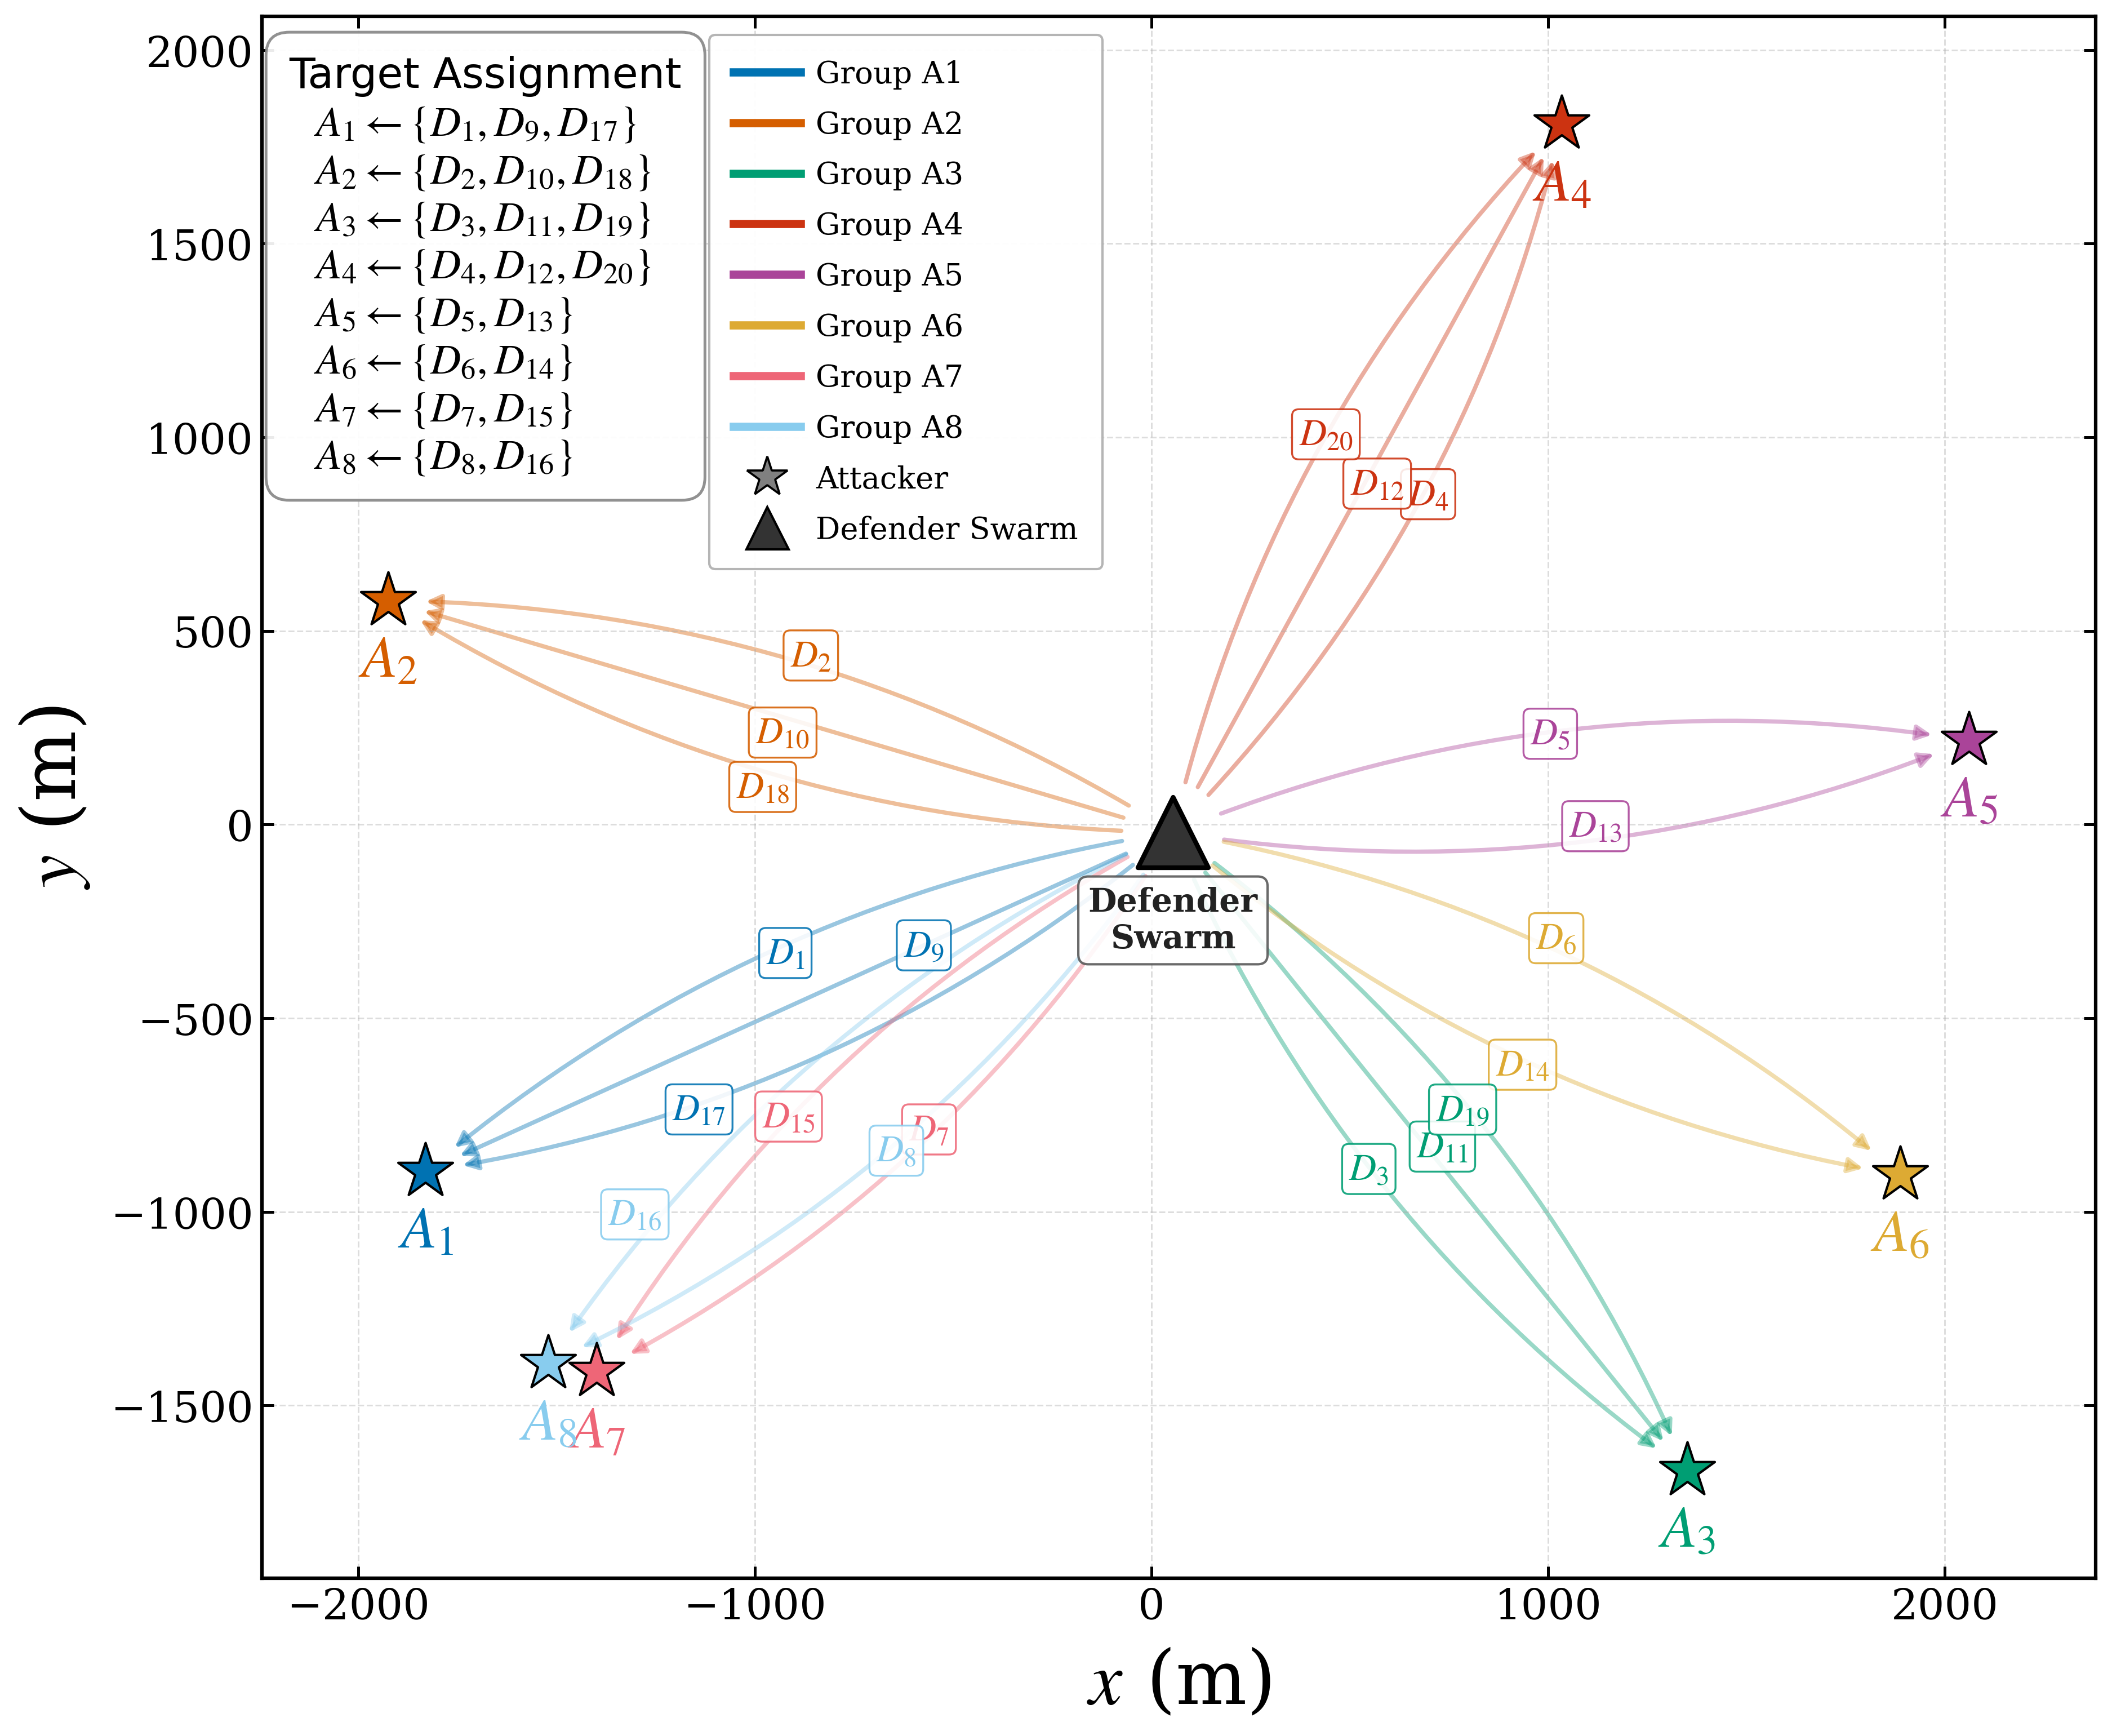
\includegraphics[width=3.2in]{target_assignment_topology.png}
\caption{Visualized spatial topology of the target assignment results.}
\label{fig:assignment_topology}
\end{figure}

To further examine the computational scalability and delay-dependent
consensus efficiency of IDBO, the nominal $20\times8$ configuration is used
as the baseline, and the scale sweep considers $10\times4$, $20\times8$,
$40\times16$, $80\times32$, and $160\times64$. Under a fixed
optimization budget, the mean CPU times are $0.031$~s, $0.048$~s, and
$1.948$~s for the representative $10\times4$, $20\times8$, and
$160\times64$ configurations, respectively. 
The observed runtime scaling is superlinear over the evaluated configurations
when the interceptor and target populations are increased concurrently.
These CPU times quantify the computational cost of
IDBO and exclude distributed communication latency.


\begin{table}[!t]
\centering
\footnotesize
\setlength{\tabcolsep}{2.8pt}
\renewcommand{\arraystretch}{1.12}
\caption{Delay-dependent consensus performance of IDBO for the
nominal $20\times8$ assignment.}
\label{tab:idbo_delay_scalability}
\begin{tabular}{@{}cccc@{}}
\hline\hline
\shortstack{Communication\\delay (ms)} &
\shortstack{Mean communication\\steps} &
\shortstack{Mean consensus\\time (s)} &
\shortstack{Consensus\\success (\%)} \\
\hline
50  & 10.6 & 0.53 & 100 \\
100 & 19.2 & 0.96 & 100 \\
150 & 27.8 & 1.39 & 100 \\
250 & 45.0 & 2.25 & 100 \\
450 & 79.4 & 3.97 & 100 \\
\hline
\end{tabular}
\end{table}

Table~\ref{tab:idbo_delay_scalability} reports the distributed
consensus performance at the nominal assignment scale. The $50$-ms case
corresponds to the nominal communication condition, while the remaining cases
provide an extended-delay evaluation. The communication-step count is measured
on the $50$-ms communication time grid. As the communication delay increased
from $50$ to $450$~ms, the mean number of communication steps required to
reach consensus increased from
$10.6$ to $79.4$, and the corresponding mean consensus time increased from
$0.53$ to $3.97$~s. Nevertheless, the consensus success rate remained
$100\%$ under all tested delays. These results show that bounded communication
delay reduces distributed consensus efficiency but does not prevent convergence
to a common conflict-free assignment under the tested conditions.








\subsection{RL Model Training and Convergence Analysis}
\label{subsec:training}

To evaluate the learning efficiency and robustness of the proposed ART-MAPPO, comparative training experiments were conducted against standard MAPPO, IPPO, IA2C, and IQL. All models were trained over 10,000 episodes with a maximum horizon of 2500 steps per episode. To ensure statistical significance and eliminate the bias of favorable network initialization, all learning curves in Fig.~\ref{fig:training_convergence} are averaged across 5 independent random seeds, with the shaded regions denoting the standard deviation.

As illustrated in Fig.~\ref{fig:training_convergence}(a), ART-MAPPO demonstrates a superior learning paradigm, achieving the highest asymptotic normalized reward of $8.97 \pm 0.64$ (averaged over the final 500 episodes). This represents a notable performance improvement of 8.2\%, 12.3\%, 14.4\%, and 29.8\% over IQL, MAPPO, IPPO, and IA2C, respectively. The advantage of ART-MAPPO is particularly pronounced during the intermediate training phase. By episode 4,000, ART-MAPPO establishes a significant performance leap, outperforming standard MAPPO by 43.6\% and IQL by 16.6\%, highlighting its ability to rapidly escape local optima early in the training process.

Furthermore, the proposed method exhibits accelerated convergence alongside enhanced training stability. When evaluated on a 100-episode smoothed curve, ART-MAPPO reaches 90\% of its optimal asymptotic performance by episode 5,591. In contrast, the most competitive baseline, IQL, requires 6,477 episodes (a 13.7\% delay), while standard MAPPO lags significantly, requiring 7,654 episodes. Regarding algorithmic stability, ART-MAPPO maintains a tight variance across random seeds ($\sigma = 0.64$), whereas standard MAPPO exhibits a standard deviation of 1.34 (approximately twice as large). This confirms that the proposed enhancements effectively mitigate the high-variance gradient updates typical in multi-agent policy-based methods.

These macroscopic performance gains are directly supported by the network-level metrics. The critic loss (Fig.~\ref{fig:training_convergence}(b)) of ART-MAPPO converges to the lowest steady-state error with minimal oscillation, a direct consequence of the dual-clip mechanism and adaptive KL penalty. Concurrently, the policy entropy (Fig.~\ref{fig:training_convergence}(c)) demonstrates an optimal, gradual decay trajectory, validating that the trust-modulated exploration mechanism successfully balances early-stage extensive state-space exploration with late-stage strict policy exploitation.

\begin{figure}[!t]
\centering
\subfloat[Training Reward]{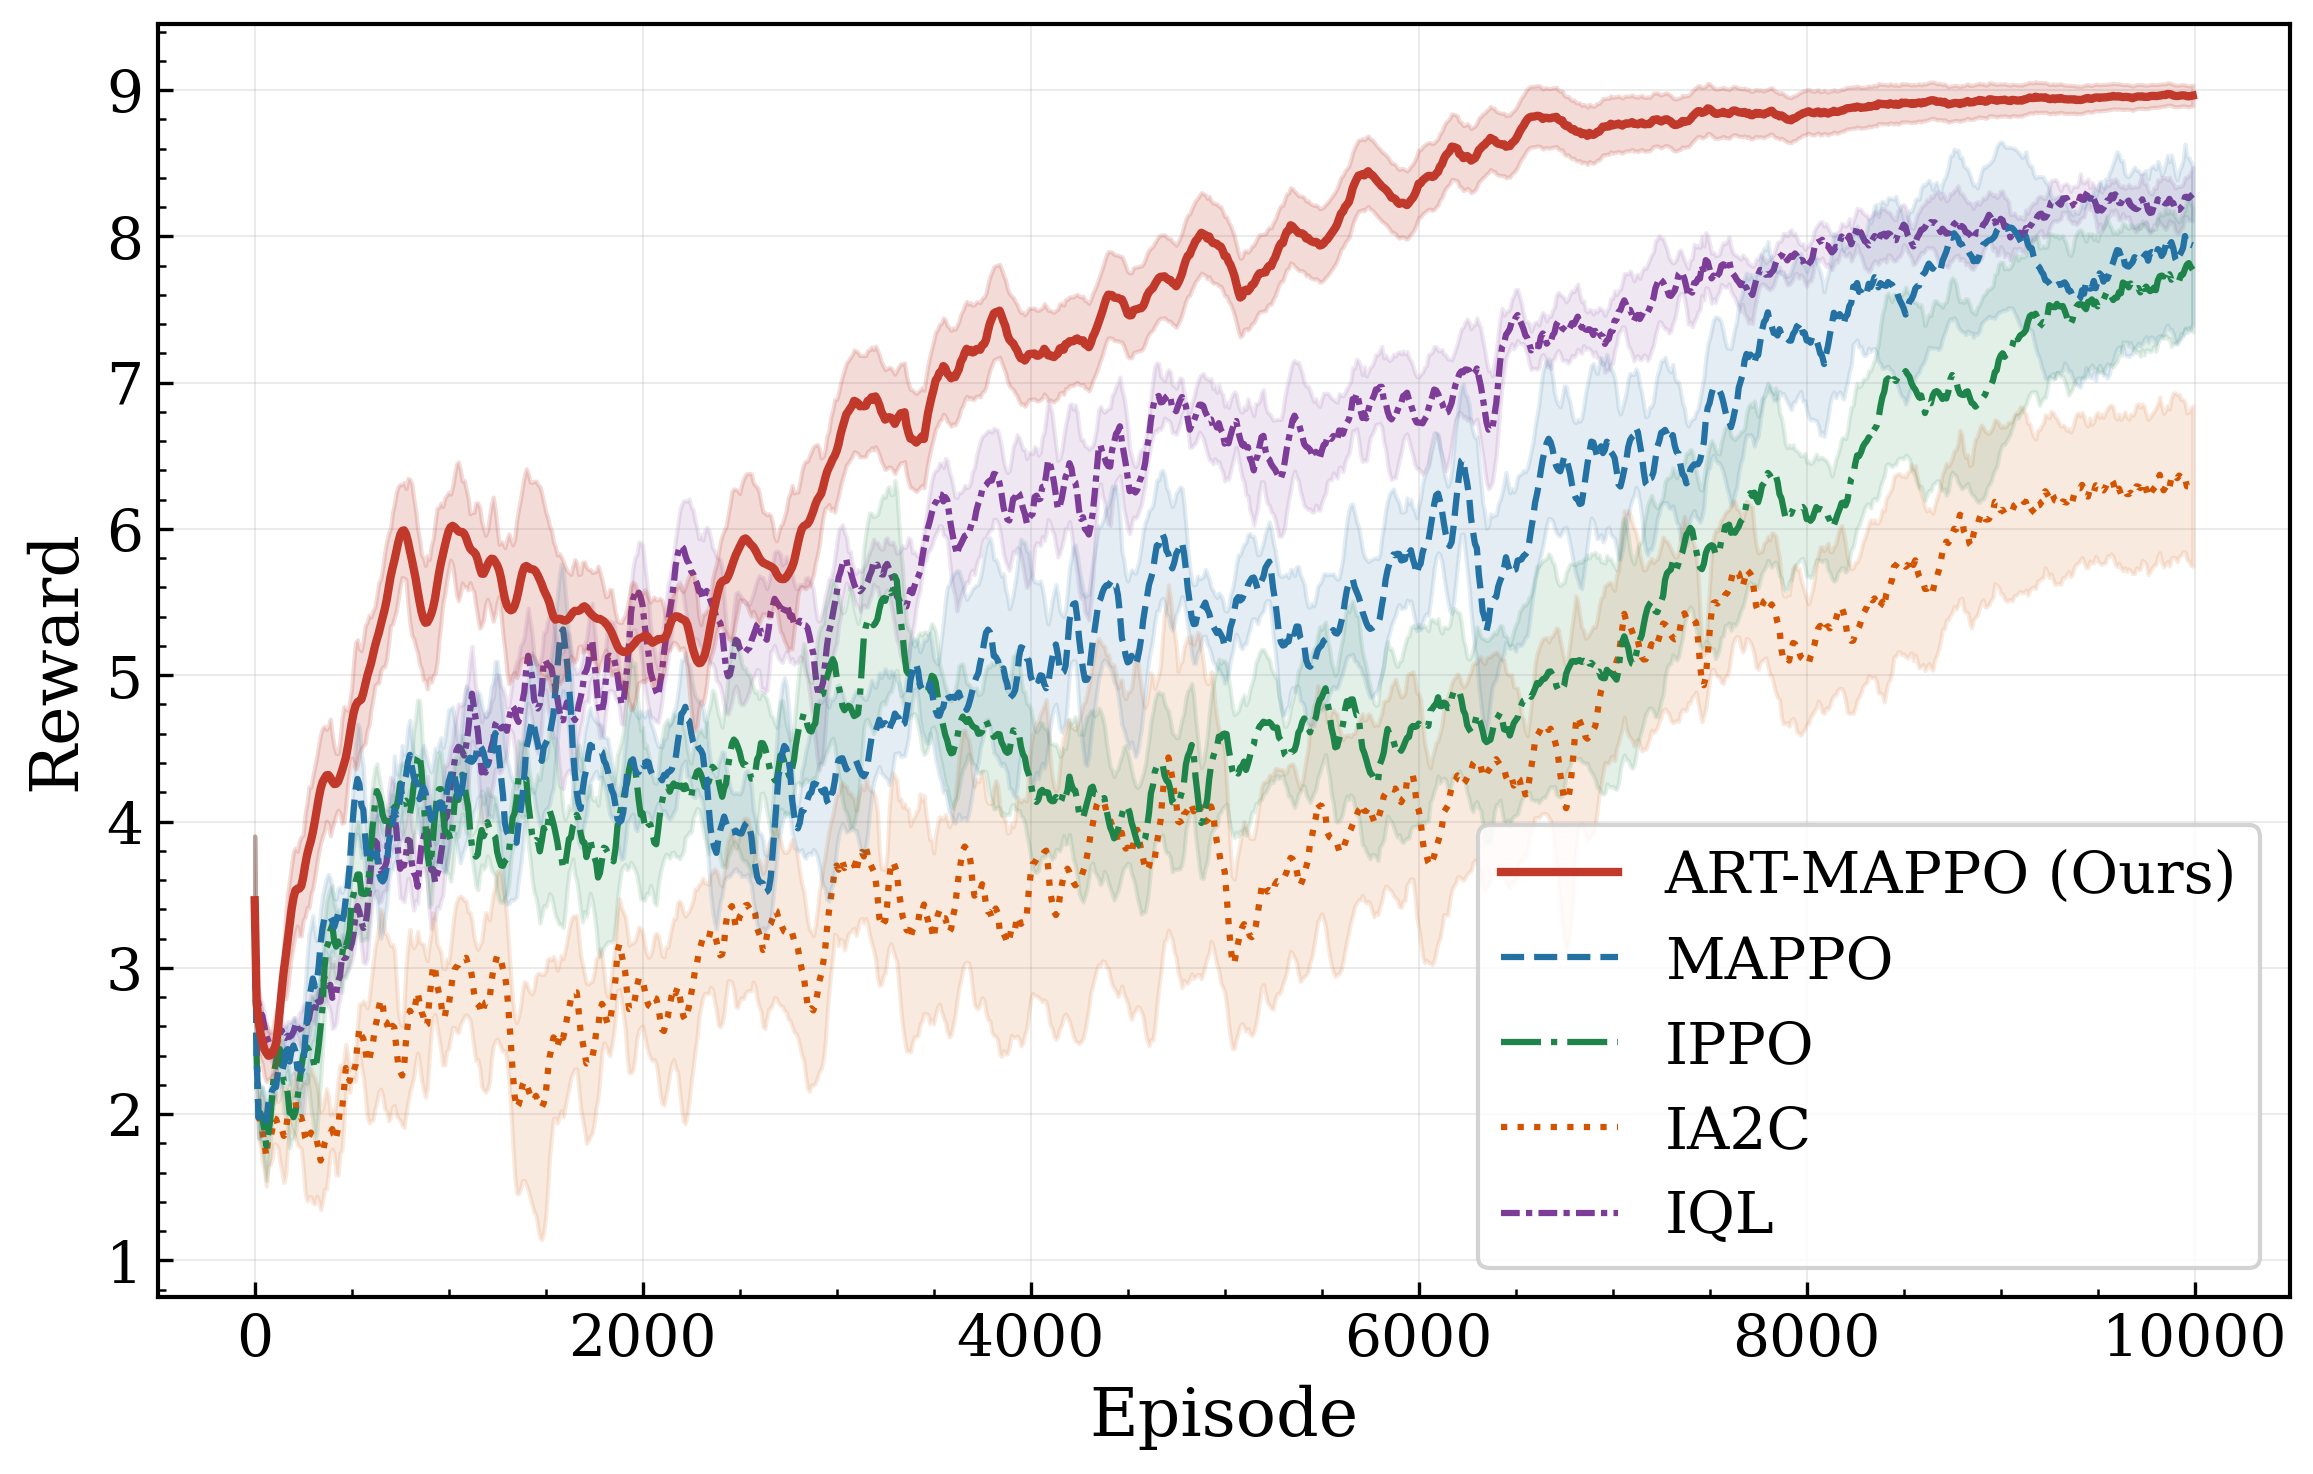
\includegraphics[width=3.0in]{fig_a_reward.png}}
\hfill
\subfloat[Critic Loss]{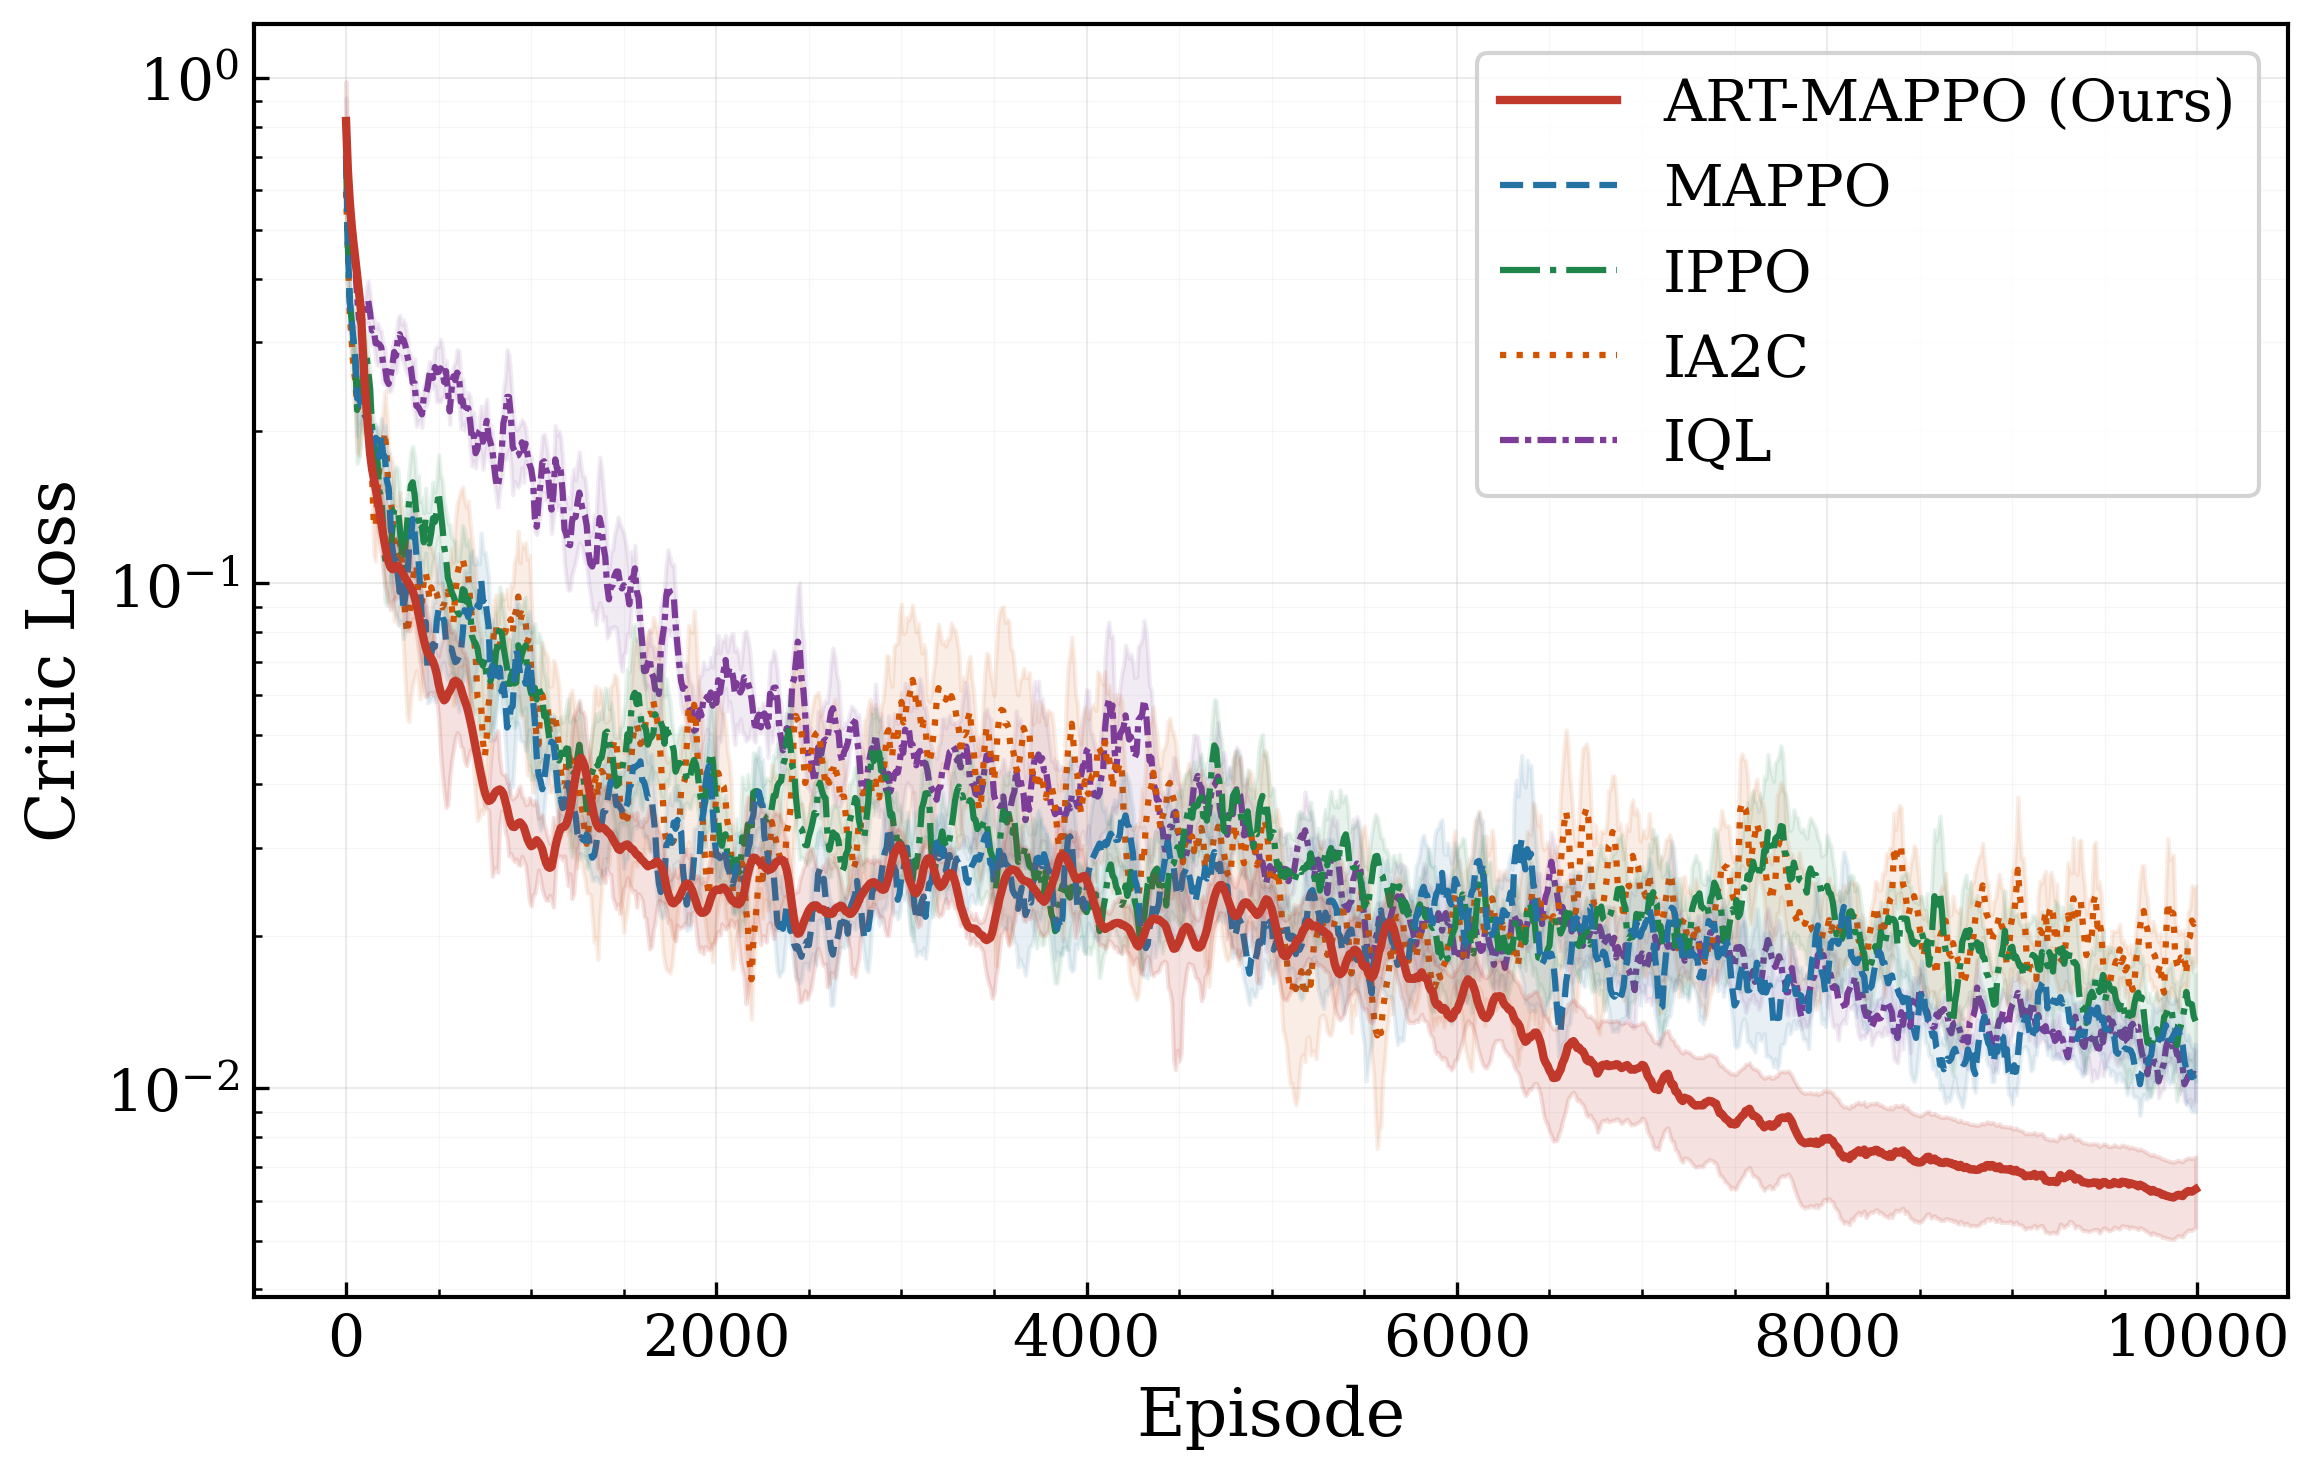
\includegraphics[width=3.0in]{fig_b_critic_loss.png}}
\hfill
\subfloat[Policy Entropy]{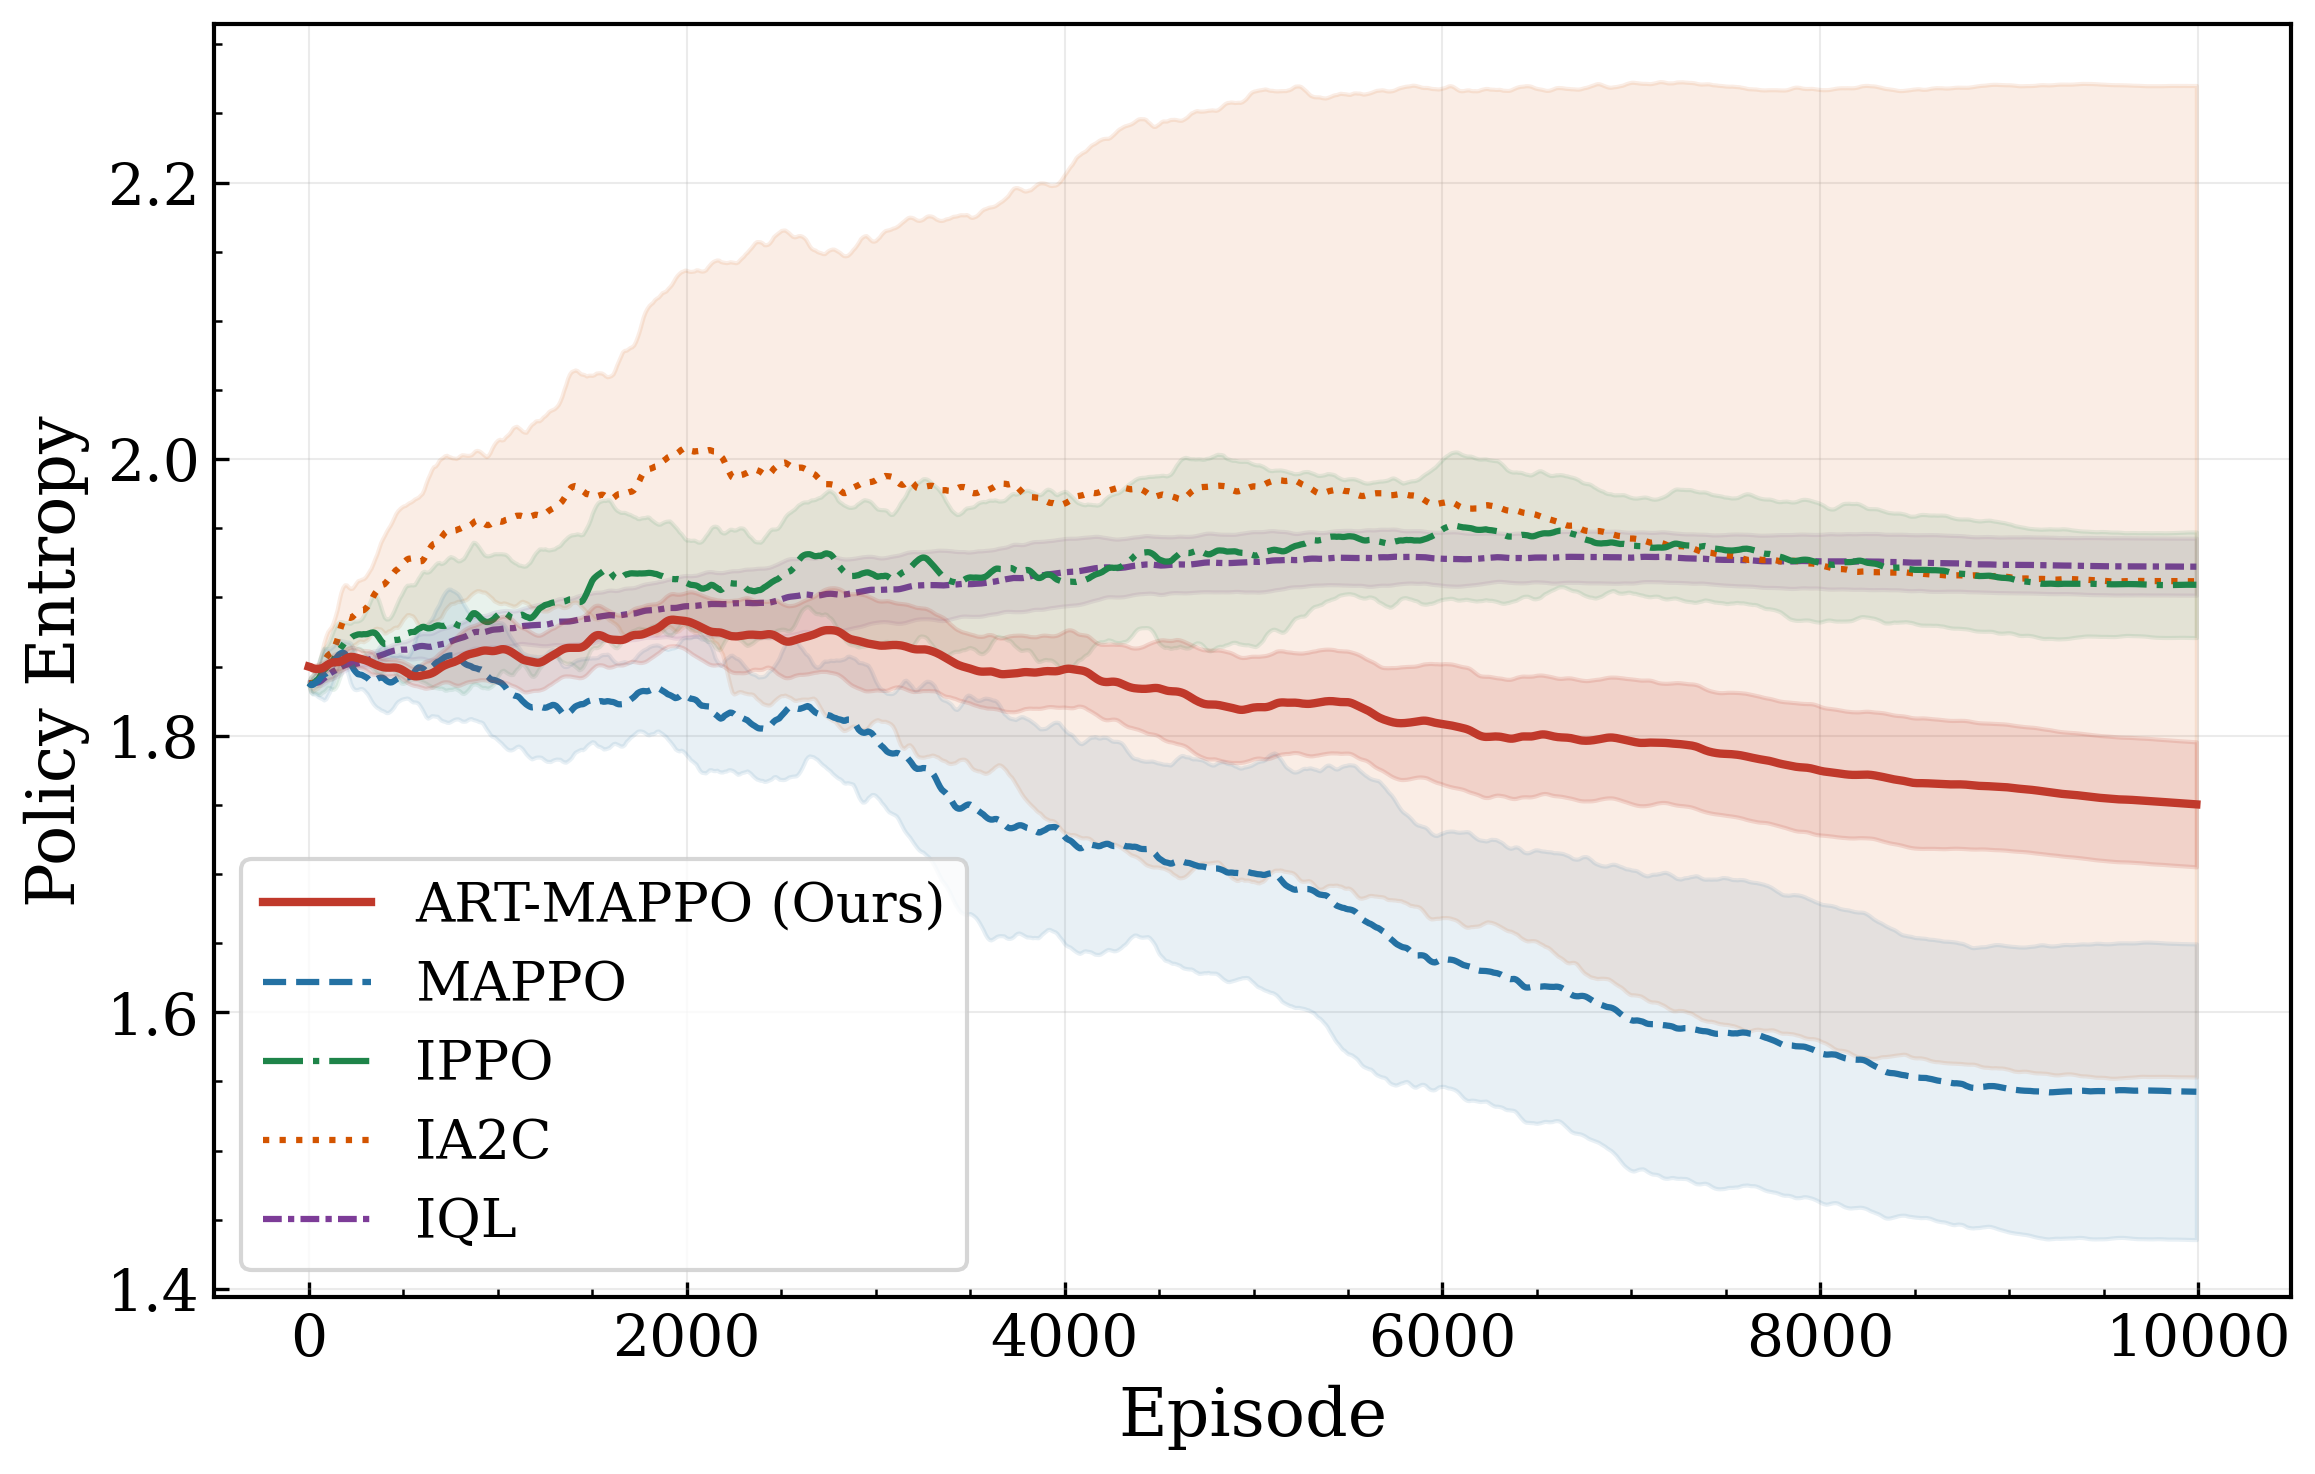
\includegraphics[width=3.0in]{fig_c_entropy.png}}
\caption{Comparative training curves of ART-MAPPO and baseline algorithms over 10,000 episodes. Solid lines and shaded regions represent the mean and standard deviation across 5 independent random seeds, respectively. Notably, ART-MAPPO achieves the highest asymptotic reward (+12.3\% over standard MAPPO) and the fastest convergence rate (reaching 90\% optimality by episode 5,591), while demonstrating significantly enhanced training stability.}
\label{fig:training_convergence}
\end{figure}


%%%%-------------------------------------------------------------------------------------------

\subsection{Cooperative Interception against Maneuvering Targets}
\label{subsec:cases}

We evaluate the complete target-assignment and terminal cooperative-guidance process
against two maneuvering scenarios, each benchmarked against classical PN.
The experiments are conducted on the HIL platform with communication delays, sensing
uncertainty and three-dimensional dynamics. The target-assignment and cooperative-guidance
modules are executed sequentially to provide end-to-end validation of the complete interception
process.



\subsubsection{Case~1: Interception against Evasive Maneuvering Targets}

In this scenario, the attacking UAVs ($A_{\text{UAV}}$) initially execute a constant-$g$ evasive maneuver and transition to proportional navigation (PN) guidance after 15\,s. This case provides an end-to-end validation in which the defending swarm performs target assignment and then executes cooperative guidance against these highly dynamic threats.

Figures~\ref{fig:case1_mappo_traj_3d} and~\ref{fig:case1_mappo_traj} illustrate the three-dimensional engagement trajectories and their two-dimensional top view, respectively. Guided by the proposed target-assignment and guidance framework, the defending swarm effectively divides into eight coordinated combat units. Despite the evasive maneuvers of the targets, ART-MAPPO generates remarkably smooth and direct pursuit curves, enabling all interceptors to successfully converge on their respective targets without unnecessary detours.

\begin{figure}[!ht]
\centering
\includegraphics[width=3.15in]{\vfig{mappo_nopn_trajectory_3d.png}}
\caption{Three-dimensional engagement trajectories of the defending swarm using ART-MAPPO
in Case~1.}
\label{fig:case1_mappo_traj_3d}
\end{figure}

\begin{figure}[!ht]
\centering
\includegraphics[width=3.15in]{\vfig{mappo_nopn_trajectory.png}}
\caption{Engagement trajectories of the defending swarm using ART-MAPPO in Case~1.}
\label{fig:case1_mappo_traj}
\end{figure}

To analyze operational efficiency and constraint adherence, Figs.~\ref{fig:case1_mappo_yaw}--\ref{fig:case1_mappo_axial} present the kinematic and control profiles of ART-MAPPO. The lateral acceleration $n_y$ in Fig.~\ref{fig:case1_mappo_yaw}(a) remains within the physical $\pm1$\,g limit throughout the mid-course and terminal phases, avoiding actuator saturation, while the heading angles smoothly approach the collision course in Fig.~\ref{fig:case1_mappo_yaw}(b). The small variations in $n_z$ and $\theta_D$ in Fig.~\ref{fig:case1_mappo_pitch} show that modest vertical corrections are sufficient to meet the three-dimensional interception requirement. The speed $V_D$ and axial acceleration $n_x$ in Fig.~\ref{fig:case1_mappo_axial} show that ART-MAPPO commands high axial acceleration early in the engagement to approach the 40\,m/s speed limit and shorten the interception duration.

\begin{figure}[!ht]
\centering
\includegraphics[width=3.1in]{\vfig{standalone_duav_legend.png}}\\[-2pt]
\subfloat[Lateral acceleration $n_y$]{\includegraphics[width=3.15in]{\vfig{mappo_nopn_ny.png}}}\\[-2pt]
\subfloat[Heading angle $\gamma_D$]{\includegraphics[width=3.15in]{\vfig{mappo_nopn_heading.png}}}
\caption{Lateral acceleration and heading-angle response of ART-MAPPO in Case~1.}
\label{fig:case1_mappo_yaw}
\end{figure}

\begin{figure}[!ht]
\centering
\includegraphics[width=3.1in]{\vfig{standalone_duav_legend.png}}\\[-2pt]
\subfloat[Normal acceleration $n_z$]{\includegraphics[width=3.15in]{\vfig{mappo_nopn_nz.png}}}\\[-2pt]
\subfloat[Flight-path angle $\theta_D$]{\includegraphics[width=3.15in]{\vfig{mappo_nopn_pitch.png}}}
\caption{Normal acceleration and flight-path-angle response of ART-MAPPO in Case~1.}
\label{fig:case1_mappo_pitch}
\end{figure}

\begin{figure}[!ht]
\centering
\includegraphics[width=3.1in]{\vfig{standalone_duav_legend.png}}\\[-2pt]
\subfloat[Axial acceleration $n_x$]{\includegraphics[width=3.15in]{\vfig{mappo_nopn_nx.png}}}\\[-2pt]
\subfloat[Velocity $V_D$]{\includegraphics[width=3.15in]{\vfig{mappo_nopn_velocity.png}}}
\caption{Axial acceleration and speed response of ART-MAPPO in Case~1.}
\label{fig:case1_mappo_axial}
\end{figure}

In stark contrast, the performance of the baseline PN guidance is presented in
Figs.~\ref{fig:case1_pn_traj_3d}--\ref{fig:case1_pn_axial}. While PN eventually
intercepts the targets (Fig.~\ref{fig:case1_pn_traj}), its purely reactive nature leads to a
highly inefficient pursuit strategy. As clearly depicted in
Fig.~\ref{fig:case1_pn_yaw}(a), the lateral acceleration ($n_y$) of PN drastically
diverges, severely violating the $\pm1$\,g physical limit because the algorithm lacks predictive
capability against evasive maneuvers, thus demanding excessive and sudden control efforts in the
terminal phase. In realistic flight conditions, such catastrophic actuator saturation would
inevitably result in structural damage or loss of control, rendering the interception a failure.
Consequently, the velocity decays significantly over time
(Fig.~\ref{fig:case1_pn_axial}(b)), dragging out the interception duration.

\begin{figure}[!ht]
\centering
\includegraphics[width=3.15in]{\pncasefig{pn_nopn_trajectory_3d.png}}
\caption{Three-dimensional engagement trajectories of the defending swarm using the PN
baseline in Case~1.}
\label{fig:case1_pn_traj_3d}
\end{figure}

\begin{figure}[!ht]
\centering
\includegraphics[width=3.15in]{\pncasefig{pn_nopn_trajectory.png}}
\caption{Engagement trajectories of the defending swarm using the PN baseline in Case~1.}
\label{fig:case1_pn_traj}
\end{figure}

\begin{figure}[!ht]
\centering
\includegraphics[width=3.1in]{\pncasefig{standalone_duav_legend.png}}\\[-2pt]
\subfloat[Lateral acceleration $n_y$]{\includegraphics[width=3.15in]{\pncasefig{pn_nopn_ny.png}}}\\[-2pt]
\subfloat[Heading angle $\gamma_D$]{\includegraphics[width=3.15in]{\pncasefig{pn_nopn_heading.png}}}
\caption{Lateral acceleration and heading-angle response of the PN baseline in Case~1.}
\label{fig:case1_pn_yaw}
\end{figure}

\begin{figure}[!ht]
\centering
\includegraphics[width=3.1in]{\pncasefig{standalone_duav_legend.png}}\\[-2pt]
\subfloat[Normal acceleration $n_z$]{\includegraphics[width=3.15in]{\pncasefig{pn_nopn_nz.png}}}\\[-2pt]
\subfloat[Flight-path angle $\theta_D$]{\includegraphics[width=3.15in]{\pncasefig{pn_nopn_pitch.png}}}
\caption{Normal acceleration and flight-path-angle response of the PN baseline in Case~1.}
\label{fig:case1_pn_pitch}
\end{figure}

\begin{figure}[!ht]
\centering
\includegraphics[width=3.1in]{\pncasefig{standalone_duav_legend.png}}\\[-2pt]
\subfloat[Axial acceleration $n_x$]{\includegraphics[width=3.15in]{\pncasefig{pn_nopn_nx.png}}}\\[-2pt]
\subfloat[Velocity $V_D$]{\includegraphics[width=3.15in]{\pncasefig{pn_nopn_velocity.png}}}
\caption{Axial acceleration and speed response of the PN baseline in Case~1.}
\label{fig:case1_pn_axial}
\end{figure}


Beyond individual interception capabilities, a core requirement of swarm defense is the execution of a simultaneous saturation strike to prevent the targets from defeating the interceptors piecemeal. This vital temporal coordination is dynamically achieved during the flight, as evidenced by the time-to-go ($t_{go}$) profiles in Fig.~\ref{fig:case1_mappo_tgo}. The $t_{go}$ curves of interceptors assigned to the same target rapidly converge as the engagement progresses. This explicitly demonstrates that ART-MAPPO actively shapes the velocity distribution of the swarm to synchronize the remaining flight times long before the actual impact.

\begin{figure}[!ht]
\centering
\includegraphics[width=3.2in]{\vfig{mappo_nopn_tgo.png}}
\caption{Time-to-go ($t_{go}$) profiles of the defending swarm using ART-MAPPO in Case~1. Interceptors assigned to the same target actively synchronize their remaining flight times to guarantee a simultaneous saturation strike.}
\label{fig:case1_mappo_tgo}
\end{figure}

Consequently, Fig.~\ref{fig:case1_time_sync} explicitly validates the ultimate temporal coordination capability by displaying the terminal arrival time difference ($\Delta t$) among the interceptors assigned to each respective target group. The maximum $\Delta t$ across all eight coordinated groups is remarkably tight, bounded to merely 0.25\,s. This quantitatively proves that the proposed framework perfectly bridges the target assignment and the trust-modulated exploration mechanisms, ensuring a strictly temporally coordinated saturation strike against the swarm threat.

\begin{figure}[!ht]
\centering
\includegraphics[width=3.0in]{\vfig{mappo_nopn_time_sync.png}}
\caption{Terminal arrival time differences $\Delta t$ within each coordinated interceptor group under ART-MAPPO. The near-zero $\Delta t$ values explicitly validate the successful execution of temporally synchronized saturation strikes.}
\label{fig:case1_time_sync}
\end{figure}







\subsubsection{Case~2: Interception against Continuous Weaving Targets}

This scenario evaluates the robustness of the proposed framework against the sinusoidal penetration maneuver~\cite{Zarchan1995969}, which represents a highly agile and continuous weaving threat. Such maneuvers induce high-frequency oscillations in the line-of-sight (LOS) rate, severely challenging both the guidance stability and the temporal coordination of the defending swarm. This case provides an end-to-end validation in which target assignment is followed by cooperative guidance against the three-dimensional weaving threats.

Figures~\ref{fig:case2_mappo_traj_3d} and~\ref{fig:case2_mappo_traj} illustrate the three-dimensional engagement trajectories and their two-dimensional top view, respectively. Despite the continuous lateral oscillations of the $A_{\text{UAV}}$, ART-MAPPO explicitly predicts and accommodates the target's weaving motion. The proposed algorithm assigns the defending UAVs to the attacking targets, forming eight coordinated combat units that successfully intercept every target with smooth pursuit curves.

\begin{figure}[!ht]
\centering
\includegraphics[width=3.15in]{\vfig{mappo_sin_trajectory_3d.png}}
\caption{Three-dimensional ART-MAPPO engagement trajectories against continuous weaving
targets in Case~2.}
\label{fig:case2_mappo_traj_3d}
\end{figure}

\begin{figure}[!ht]
\centering
\includegraphics[width=3.15in]{\vfig{mappo_sin_trajectory.png}}
\caption{Engagement trajectories of the defending swarm using ART-MAPPO against continuous weaving targets in Case~2.}
\label{fig:case2_mappo_traj}
\end{figure}

The kinematic and control responses of ART-MAPPO are further detailed in Figs.~\ref{fig:case2_mappo_yaw}--\ref{fig:case2_mappo_axial}. To counter the weaving targets, ART-MAPPO generates an adaptive oscillatory lateral-acceleration command $n_y$ while remaining within the safe $\pm1$\,g envelope, and it adjusts the heading angle smoothly, as shown in Fig.~\ref{fig:case2_mappo_yaw}. The small variations in $n_z$ and $\theta_D$ in Fig.~\ref{fig:case2_mappo_pitch} show that modest vertical corrections are sufficient to meet the three-dimensional interception requirement. As in Case~1, the axial acceleration $n_x$ is used to increase the approach speed, as shown in Fig.~\ref{fig:case2_mappo_axial}.

\begin{figure}[!ht]
\centering
\includegraphics[width=3.1in]{\vfig{standalone_duav_legend.png}}\\[-2pt]
\subfloat[Lateral acceleration $n_y$]{\includegraphics[width=3.15in]{\vfig{mappo_sin_ny.png}}}\\[-2pt]
\subfloat[Heading angle $\gamma_D$]{\includegraphics[width=3.15in]{\vfig{mappo_sin_heading.png}}}
\caption{Lateral acceleration and heading-angle response of ART-MAPPO in Case~2.}
\label{fig:case2_mappo_yaw}
\end{figure}

\begin{figure}[!ht]
\centering
\includegraphics[width=3.1in]{\vfig{standalone_duav_legend.png}}\\[-2pt]
\subfloat[Normal acceleration $n_z$]{\includegraphics[width=3.15in]{\vfig{mappo_sin_nz.png}}}\\[-2pt]
\subfloat[Flight-path angle $\theta_D$]{\includegraphics[width=3.15in]{\vfig{mappo_sin_pitch.png}}}
\caption{Normal acceleration and flight-path-angle response of ART-MAPPO in Case~2.}
\label{fig:case2_mappo_pitch}
\end{figure}

\begin{figure}[!ht]
\centering
\includegraphics[width=3.1in]{\vfig{standalone_duav_legend.png}}\\[-2pt]
\subfloat[Axial acceleration $n_x$]{\includegraphics[width=3.15in]{\vfig{mappo_sin_nx.png}}}\\[-2pt]
\subfloat[Velocity $V_D$]{\includegraphics[width=3.15in]{\vfig{mappo_sin_velocity.png}}}
\caption{Axial acceleration and speed response of ART-MAPPO in Case~2.}
\label{fig:case2_mappo_axial}
\end{figure}

Conversely, the PN baseline completely fails to handle the high-frequency dynamic engagement
geometry. The reactive nature of PN results in phase-lagged trajectories that struggle to close
the distance (Fig.~\ref{fig:case2_pn_traj}). As revealed in the control profiles
(Figs.~\ref{fig:case2_pn_yaw}--\ref{fig:case2_pn_axial}), the PN guidance law
suffers from catastrophic actuator saturation during the terminal phase. Specifically, the
lateral-acceleration commands ($n_y$) frequently breach the $\pm 1$\,g limit
(Fig.~\ref{fig:case2_pn_yaw}(a)), which would severely compromise flight safety
and render the interception a failure in real-world applications.

\begin{figure}[!ht]
\centering
\includegraphics[width=3.15in]{\pncasefig{pn_sin_trajectory_3d.png}}
\caption{Three-dimensional engagement trajectories of the defending swarm using the PN
baseline in Case~2.}
\label{fig:case2_pn_traj_3d}
\end{figure}

\begin{figure}[!ht]
\centering
\includegraphics[width=3.15in]{\pncasefig{pn_sin_trajectory.png}}
\caption{Engagement trajectories of the defending swarm using the PN baseline in Case~2.}
\label{fig:case2_pn_traj}
\end{figure}

\begin{figure}[!ht]
\centering
\includegraphics[width=3.1in]{\pncasefig{standalone_duav_legend.png}}\\[-2pt]
\subfloat[Lateral acceleration $n_y$]{\includegraphics[width=3.15in]{\pncasefig{pn_sin_ny.png}}}\\[-2pt]
\subfloat[Heading angle $\gamma_D$]{\includegraphics[width=3.15in]{\pncasefig{pn_sin_heading.png}}}
\caption{Lateral acceleration and heading-angle response of the PN baseline in Case~2.}
\label{fig:case2_pn_yaw}
\end{figure}

\begin{figure}[!ht]
\centering
\includegraphics[width=3.1in]{\pncasefig{standalone_duav_legend.png}}\\[-2pt]
\subfloat[Normal acceleration $n_z$]{\includegraphics[width=3.15in]{\pncasefig{pn_sin_nz.png}}}\\[-2pt]
\subfloat[Flight-path angle $\theta_D$]{\includegraphics[width=3.15in]{\pncasefig{pn_sin_pitch.png}}}
\caption{Normal acceleration and flight-path-angle response of the PN baseline in Case~2.}
\label{fig:case2_pn_pitch}
\end{figure}

\begin{figure}[!ht]
\centering
\includegraphics[width=3.1in]{\pncasefig{standalone_duav_legend.png}}\\[-2pt]
\subfloat[Axial acceleration $n_x$]{\includegraphics[width=3.15in]{\pncasefig{pn_sin_nx.png}}}\\[-2pt]
\subfloat[Velocity $V_D$]{\includegraphics[width=3.15in]{\pncasefig{pn_sin_velocity.png}}}
\caption{Axial acceleration and speed response of the PN baseline in Case~2.}
\label{fig:case2_pn_axial}
\end{figure}

The continuous maneuvering of the targets also disrupts conventional coordination mechanisms. However, this vital temporal synchronization is dynamically sustained by ART-MAPPO during the flight, as evidenced by the time-to-go ($t_{go}$) profiles in Fig.~\ref{fig:case2_mappo_tgo}. Even against severe LOS oscillations, the $t_{go}$ curves of interceptors assigned to the same target smoothly converge. This demonstrates that the algorithm continuously and intelligently adapts the swarm's velocity distribution to lock in synchronized impact times, despite the highly dynamic nature of the weaving threats.

\begin{figure}[!ht]
\centering
\includegraphics[width=3.2in]{\vfig{mappo_sin_tgo.png}}
\caption{Time-to-go ($t_{go}$) profiles of the defending swarm using ART-MAPPO in Case~2. Interceptors actively synchronize their remaining flight times despite the continuous high-G maneuvers of the targets.}
\label{fig:case2_mappo_tgo}
\end{figure}

Consequently, the ultimate validation of ART-MAPPO's saturation strike capability under extreme dynamic conditions is explicitly presented in Fig.~\ref{fig:case2_time_sync}. Even against highly evasive sinusoidal targets, the maximum terminal arrival time difference ($\Delta t$) among the coordinated groups is strictly bounded to 0.30\,s. This exceptional synchronization quantitatively confirms the superiority of the ART-MAPPO framework in executing temporally coordinated saturation strikes in highly complex adversarial environments.

\begin{figure}[!ht]
\centering
\includegraphics[width=3.0in]{\vfig{mappo_sin_time_sync.png}}
\caption{Terminal arrival time differences $\Delta t$ for Case~2. The remarkably low variance ($\le 0.30$\,s) proves that ART-MAPPO preserves strict temporal synchronization even against continuous weaving targets.}
\label{fig:case2_time_sync}
\end{figure}

% \FloatBarrier

% Component Ablation Study — Re2_6
\subsection{Component Ablation Study}
\label{subsec:ablation}

To isolate the independent contribution of each proposed component, we construct three
one-at-a-time ablation controls alongside the complete ART-MAPPO model.
\emph{``w/o trust-aware mechanism''} disables the trust-modulated fusion of the analytical
guidance prior and the learned action; \emph{``w/o GRU temporal encoder''} replaces recurrent
state encoding with a memoryless feedforward layer; \emph{``w/o attention--residual backbone''}
substitutes a parameter-matched feedforward network while retaining the trust and GRU modules.
All variants share the same reward, dynamics, optimiser, training seed, and budget, and are
evaluated in 1000 frozen-policy Case~1 Monte Carlo trials.  Table~\ref{tab:ablation_case1}
summarises the results.  Critically, the three controls exhibit \emph{module-specific} rather
than uniformly ordered degradation, providing direct evidence that each component carries a
distinct and non-redundant role.

\begin{table*}[!t]
\centering

\small
\caption{Component ablation of ART-MAPPO: 1000-trial Case~1 Monte Carlo evaluation.}
\label{tab:ablation_case1}
\renewcommand{\arraystretch}{1.12}
\setlength{\tabcolsep}{3.5pt}
\begin{tabular}{lccccccc}
\toprule
Variant
  & Training AUC ($10^4$) $\uparrow$
  & Final reward $\uparrow$
  & ISR (\%) $\uparrow$
  & $E_{co\text{-}time}$ (s) $\downarrow$
  & $E_n$ (g) $\downarrow$
  & $E_t$ (s) $\downarrow$
  & $E_{miss}$ (m) $\downarrow$ \\
\midrule
Full ART-MAPPO                   & 7.354 & 8.958 & \textbf{98.7} & 0.0505 & 0.0718 & 28.843 & 2.997 \\
w/o trust-aware mechanism        & 6.037 & 8.683 & 97.2          & 0.0545 & 0.0739 & 29.132 & 3.087 \\
w/o GRU temporal encoder         & 6.388 & 8.134 & 95.8          & 0.0732 & 0.0782 & 30.574 & 3.297 \\
w/o attention--residual backbone & 6.651 & 8.353 & 96.1          & 0.0606 & 0.0847 & 29.853 & 3.507 \\
\bottomrule
\end{tabular}
\end{table*}

\emph{(i) Trust-aware mechanism.}  Removing trust produces the largest training-AUC
reduction among the three controls ($-17.9\%$, from $7.354\!\times\!10^4$ to
$6.037\!\times\!10^4$), yet the final reward falls by only $3.1\%$ and ISR drops by
$1.5$~pp.  The pronounced gap between cumulative-AUC loss and end-of-training reward confirms
that the trust-aware mechanism primarily accelerates learning efficiency throughout training,
not merely raises the asymptotic policy ceiling---consistent with its design role of
dynamically regulating exploration--exploitation balance.

\emph{(ii) GRU temporal encoder.}  The GRU removal yields the lowest final reward
($-9.2\%$) and the largest ISR degradation ($-2.9$~pp) among all controls.  Most
distinctively, $E_{co\text{-}time}$ increases by $45\%$ (from $0.0505$~s to $0.0732$~s),
far exceeding the $6\%$ increase in $E_t$.  Without temporal history, the policy can no
longer reliably track target manoeuvres or reconcile interceptor time-to-go estimates,
leading to simultaneous degradation in both final policy quality and cooperative timing
precision.

\emph{(iii) Attention--residual backbone.}  Removing the attentive backbone yields the
largest increases in $E_n$ ($+18\%$, from $0.0718$~g to $0.0847$~g) and $E_{miss}$
($+17\%$, from $2.997$~m to $3.507$~m) across all three ablations, while $E_t$ changes by
only $3.5\%$.  This non-uniform degradation demonstrates that the backbone contributes
primarily to control-relevant feature extraction and terminal precision rather than
engagement duration---matching its theoretical role of resolving the coupled LOS,
relative-motion, and time-to-go state features needed for low-lateral-acceleration precision guidance.

\subsection{Monte Carlo Statistical Analysis and Robustness}
\label{subsec:montecarlo}

To rigorously quantify the robustness of the proposed framework, 1000 independent Monte Carlo trials are conducted for each case. It is important to note that the statistical distributions presented in Fig.~\ref{fig:mc_boxplots} ($E_{co\text{-}time}$, $E_n$, $E_{miss}$, and $E_t$) are exclusively derived from the successful interception trials. Specifically, out of the 1000 trials in Case~1, ART-MAPPO and PN successfully intercepted the targets 987 and 944 times, respectively. In the highly dynamic Case~2, ART-MAPPO maintained a remarkable 971 successful interceptions, whereas the baseline PN succeeded only 175 times.
% It is worth noting that under combined observation delay ($0.3$~s) and measurement noise ($\sigma_p{=}3$~m, $\sigma_v{=}0.3$~m/s), the cooperative interception success rates decrease to $42.5\%$ (Case~1) and $39.8\%$ (Case~2), indicating the sensitivity limit of the framework under coupled sensor and actuator imperfections.}

\begin{figure}[!t]
\centering
\subfloat[Case~1]{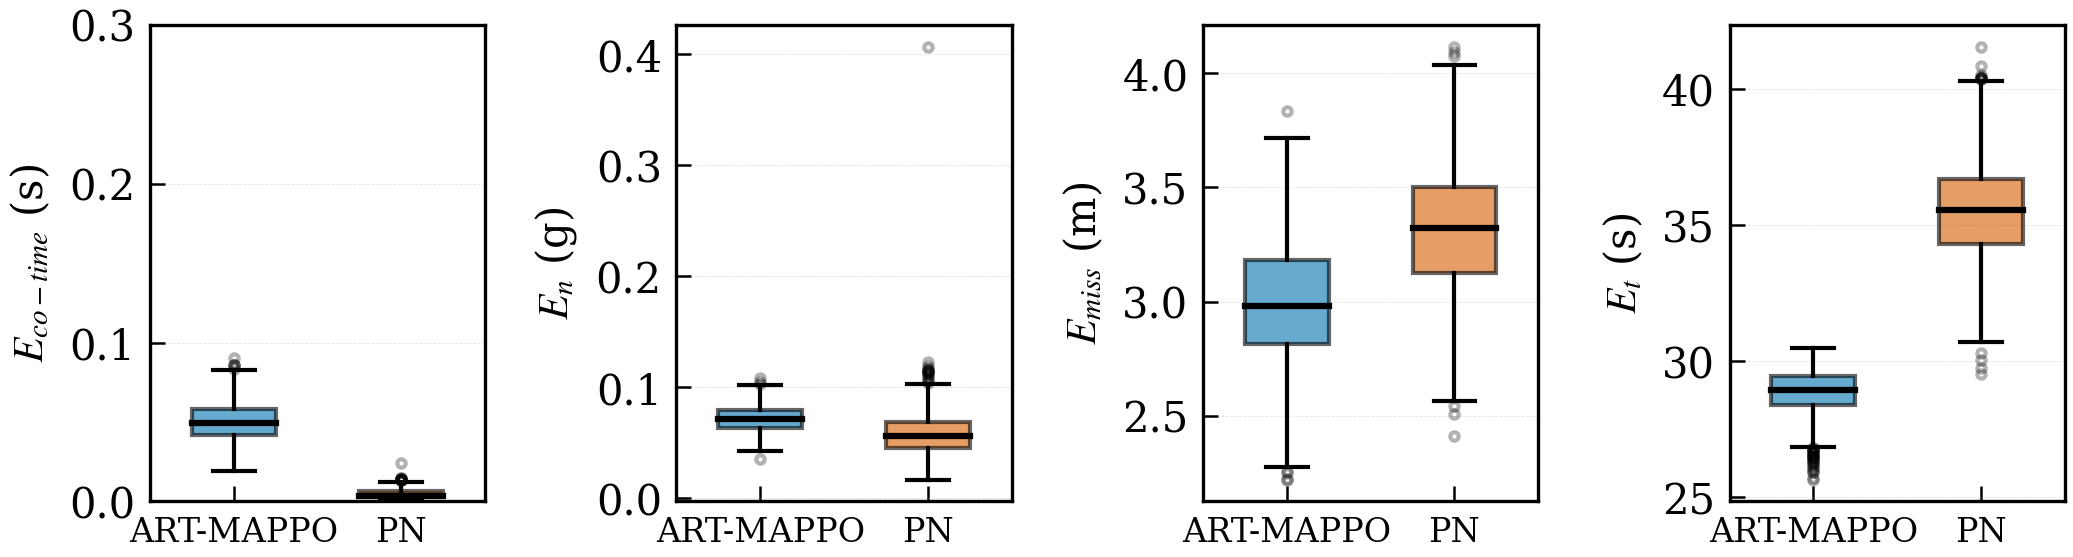
\includegraphics[width=3.5in]{nopn_mc_boxplot_compare.png}}\\
\subfloat[Case~2]{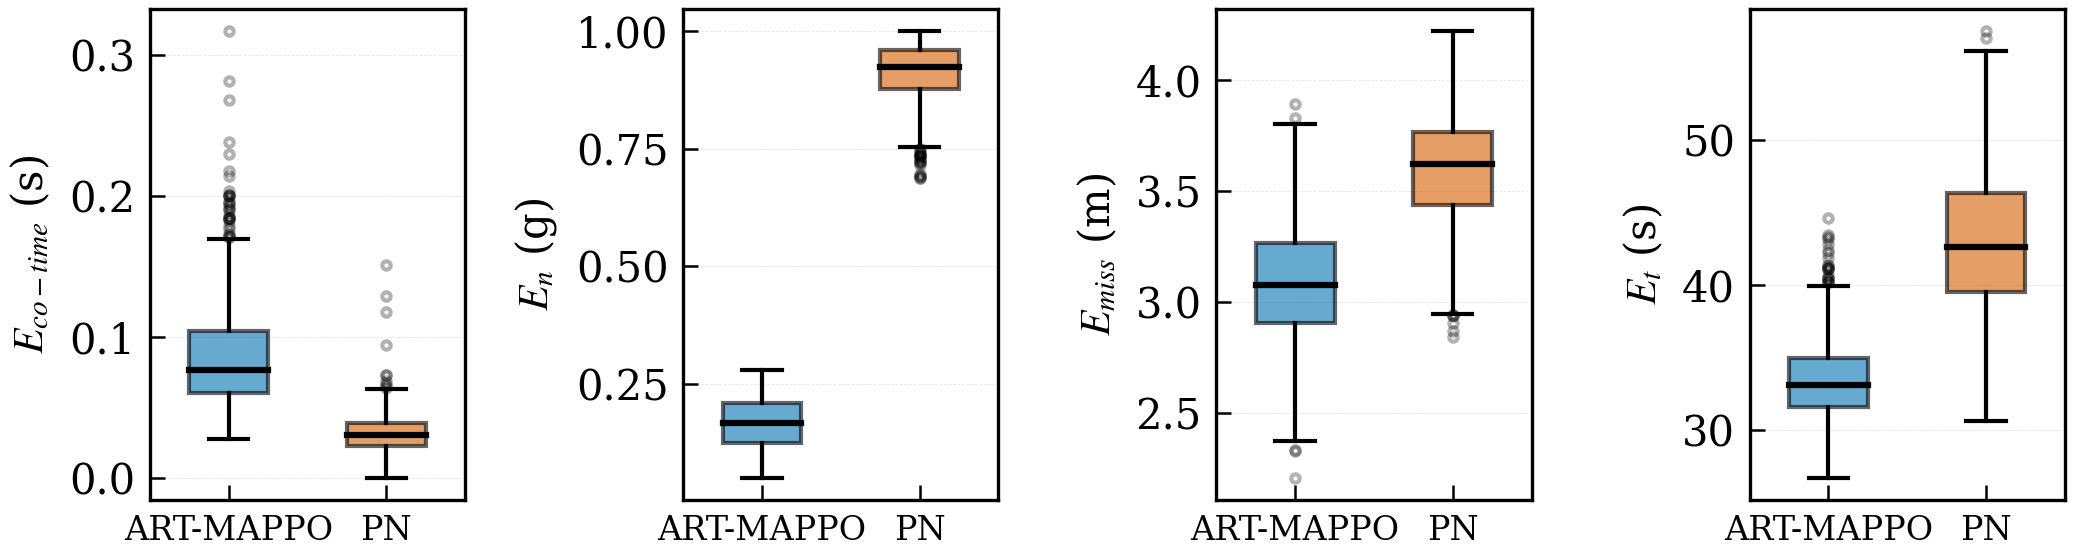
\includegraphics[width=3.5in]{sin_mc_boxplot_compare.png}}
\caption{Boxplots of Monte Carlo trials comparing ART-MAPPO and PN (data derived from successful interceptions).}
\label{fig:mc_boxplots}
\end{figure}

Based on the statistical distributions, three key findings emerge:

\emph{(i) Interception reliability and precision.} The Interception Success Rates (ISRs) directly reflect the algorithms' adaptability to aggressive target maneuvers. While PN achieves a respectable 94.40\% against the evasive target (Case~1), its performance precipitously degrades to 17.50\% when facing the continuous weaving target (Case~2). Conversely, ART-MAPPO sustains exceptional ISRs of 98.7\% and 97.1\%, demonstrating profound robustness against continuous, high-frequency line-of-sight (LOS) oscillations. Furthermore, the $E_{miss}$ boxplots confirm that ART-MAPPO consistently achieves a lower median miss distance with a significantly narrower interquartile range (IQR), ensuring lethal precision even under worst-case initializations.
Failure-case analysis was conducted on the 13 unsuccessful trials in
Case~1 and 29 in Case~2. For unsuccessful interception, the interceptor
swarm starts from an unfavorable engagement geometry, with its initial flight
direction differing substantially from the incoming direction of the
attacking swarm. Sustained target maneuvering further prolongs the required
trajectory correction and reduces the effective closing rate, preventing an
interceptor from intercepting the incoming target before it reaches the
high-value target area. For delayed cooperative engagement, differences in
path length and maneuver-induced detours maintain the time-to-go dispersion
within a target group, causing one interceptor to arrive late although the
target is eventually intercepted. The former results from the loss of
effective closure under unfavorable initial heading geometry and sustained
target maneuvering, whereas the latter results from persistent within-group
time-to-go differences caused by path asymmetry.

\emph{(ii) Terminal lateral acceleration and operational efficiency.} The metric $E_n$ denotes the terminal lateral acceleration, which is a critical constraint for flight safety. As depicted in the boxplots, ART-MAPPO's $E_n$ is tightly clustered around a safe median of $\approx0.08$\,g (Case~1) and $\approx0.20$\,g (Case~2). In contrast, particularly in Case~2, PN's $E_n$ distribution is concentrated near the 1.0\,g upper bound, exposing severe terminal actuator saturation as PN reacts to the sinusoidal maneuvers. Additionally, ART-MAPPO bounds the engagement duration $E_t$ within a tight and predictable time window, reflecting effective forward-energy management and rapid closure.

\emph{(iii) Robust temporal coordination.} The metric $E_{co\text{-}time}$ evaluates the temporal synchronization of the defending swarm. Across the successful Monte Carlo trials in both highly dynamic scenarios, ART-MAPPO maintains a median $E_{co\text{-}time}$ well below 0.10\,s. This consistently tight distribution confirms that the proposed algorithm can reliably shape the swarm's velocity profile to satisfy the strict temporal requirements for simultaneous saturation strikes, effectively neutralizing the risk of sequential piecemeal defeat.

\emph{(iv) Generalization to unseen attack patterns.} To further evaluate the proposed method under unseen attack patterns, additional Monte Carlo experiments were conducted in Case~3, where the attackers adopted bang--bang evasion. Over $1{,}000$ independent trials, the proposed method achieves a cooperative interception success rate of $96.4\%$, with $E_{co\text{-}time}=0.051$~s and $E_{miss}=1.44$~m, demonstrating effective temporal coordination and terminal accuracy under this additional maneuvering threat (Fig.~\ref{fig:case4_metrics}).

\begin{figure}[!t]
\centering
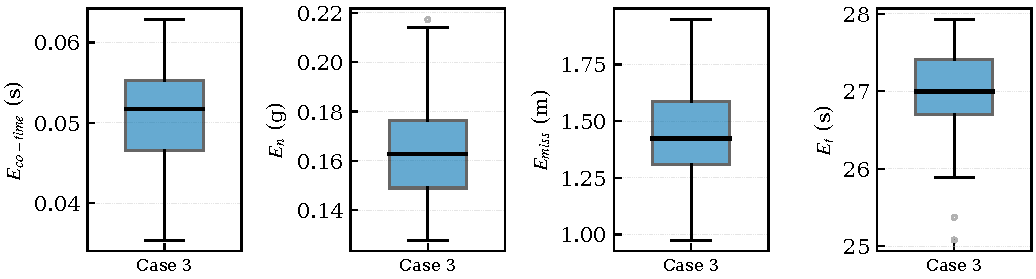
\includegraphics[width=3.5in]{case3_bangbang_metrics_box4.pdf}
\caption{Guidance-quality metric distributions for the unseen Case~3 bang-bang scenario
($1{,}000$~trials, $96.4\%$ ISR): (a)~$E_{co\text{-}time}$, (b)~$E_n$, (c)~$E_{miss}$,
(d)~$E_t$. Diamonds mark means.}
\label{fig:case4_metrics}
\end{figure}


\emph{(v) Robustness to partial interceptor failures.}
To evaluate robustness to partial interceptor failures, 1,000 end-to-end
Monte Carlo trials are conducted for each case. In each trial, two
interceptors are randomly designated as failed, and the IDBO module
constructs a new assignment using the remaining interceptors. The resulting
allocation preserves complete target coverage, after which the surviving
interceptor swarm performs cooperative guidance using ART-MAPPO.

Despite the reduced number of available interceptors, the proposed algorithm
achieves ISRs of $95.4\%$ in Case~1 and $93.9\%$ in Case~2. The statistical
distributions in Fig.~\ref{fig:partial_failure_metrics} further show that
the surviving swarm retains terminal accuracy and effective temporal
coordination while requiring relatively low terminal lateral acceleration.
These results demonstrate that the proposed algorithm maintains stable
cooperative interception performance under partial interceptor failures.

\begin{figure}[!t]
\centering
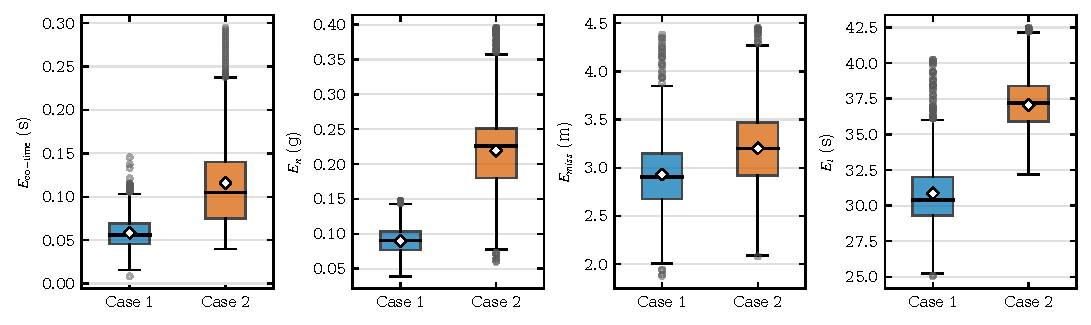
\includegraphics[width=3.5in]{partial_interceptor_failure_reference_v5_boxplots_real.pdf}
\caption{Performance distributions under two-interceptor failures in Cases~1 and~2.}
\label{fig:partial_failure_metrics}
\end{figure}




%% ===========================================================
\subsection{Parameter Sensitivity Analysis}
\label{subsec:parameter_sensitivity}

% \emph{1) IDBO Assignment-Weight Sensitivity.}
% The interception probability is $P_{ij}=w_1 P_{\mathrm{ZEM}}(i,j)+w_2 P_{\sigma}(i,j)$
% with $w_1+w_2=1$, so a single scalar $w_1$ determines the tactical priority.
% To quantify this trade-off, $w_1$ is swept over $21$ equally-spaced points in $[0,1]$
% (step $0.05$) with $12$ independent random engagement geometries ($20$ defenders,
% $8$ attackers, following the scenario in Table~\ref{chushicanshu}), and the results
% are averaged. Table~\ref{tab:sensitivity_assign} reports a representative subsample
% of the sweep. Increasing $w_1$ drives reachability: the mean selected ZEM drops from
% $1{,}152$\,m at $w_1{=}0$ to $676$\,m at $w_1{=}1.0$ (a $41.3\%$ reduction), while the
% mean three-dimensional angular error of the selected interceptor--target pairs rises
% from $65.3^{\circ}$ to $93.5^{\circ}$, passing through a shallow minimum of
% $61.6^{\circ}$ near $w_1{\approx}0.15$. The aggregate effectiveness stays robust: the
% expected number of surviving targets $J$ remains within $[0.032,0.178]$ across the
% entire sweep ($\geq\!97.8\%$ expected neutralization everywhere). The nominal setting
% $w_1{=}0.55$ is chosen as the min--max balance of the two normalized tactical costs,
% yielding a favorable compromise ($J{=}0.164$, mean ZEM $785$\,m, mean angular error
% $71.8^{\circ}$) rather than optimizing either cost alone.}

% \begin{table}[!t]
% \centering
% \renewcommand{\arraystretch}{1.15}
% \caption{IDBO Assignment-Weight Sensitivity vs.\ $w_1$ ($w_2{=}1{-}w_1$;
% Subsampled From the 21-Point Sweep; Nominal $w_1{=}0.55$ in Bold)}}
% \label{tab:sensitivity_assign}
% {
% \begin{tabular}{cccc}
% \hline\hline
% $w_1$ & Mean ZEM (m) & Mean 3-D ang.\ err.\ ($^{\circ}$) & $J$ (of $8$) \\ \hline
% 0.00 & 1152 & 65.3 & 0.066 \\
% 0.10 & 1061 & 62.1 & 0.101 \\
% 0.20 & 1004 & 63.0 & 0.131 \\
% 0.30 & 936  & 63.3 & 0.146 \\
% 0.40 & 889  & 65.9 & 0.168 \\
% 0.50 & 827  & 69.3 & 0.176 \\
% \textbf{0.55} & \textbf{785} & \textbf{71.8} & \textbf{0.164} \\
% 0.60 & 762  & 73.8 & 0.157 \\
% 0.70 & 755  & 77.0 & 0.144 \\
% 0.80 & 701  & 79.7 & 0.102 \\
% 0.90 & 667  & 84.1 & 0.066 \\
% 1.00 & 676  & 93.5 & 0.032 \\
% \hline
% \end{tabular}
% }
% \end{table}






\emph{1) IDBO Assignment-Weight Sensitivity.}
The coefficients $w_{1,\mathrm{IDBO}}$ and $w_{2,\mathrm{IDBO}}$ represent
the relative emphasis on interception reachability and three-dimensional
engagement geometry, respectively. The sensitivity analysis is conducted in
Case~1 using 1,000 end-to-end Monte Carlo trials for each setting. As shown
in Table~\ref{tab:sensitivity_assign}, larger $w_{1,\mathrm{IDBO}}$ tends
to reduce $E_{co\text{-}time}$ because reachability-oriented assignments
require less arrival-time adjustment, although the resulting engagement
geometry may demand greater terminal acceleration and prolong the
interception. Increasing $w_{2,\mathrm{IDBO}}$ improves the approach
geometry and reduces the maneuvering demand, but the weaker emphasis on
reachability increases the difficulty of temporal coordination. The growth
of $E_{miss}$ toward either end of the weighting range shows that terminal
accuracy deteriorates when either assignment criterion is excessively
emphasized.


\begin{table}[!t]
\centering
\scriptsize
\setlength{\tabcolsep}{1.8pt}
\renewcommand{\arraystretch}{1.15}
\caption{Sensitivity Analysis of the IDBO Assignment-Probability
Weighting Coefficients.}
\label{tab:sensitivity_assign}
{
\resizebox{\columnwidth}{!}{%
\begin{tabular}{@{}cccccccc@{}}
\hline\hline
\shortstack{\phantom{X}\\$w_{1,\mathrm{IDBO}}$\\\phantom{X}}
&
\shortstack{\phantom{X}\\$w_{2,\mathrm{IDBO}}$\\\phantom{X}}
&
\shortstack{Mean\\ZEM (m)\\$\downarrow$}
&
\shortstack{Mean 3-D\\angular error ($^\circ$)\\$\downarrow$}
&
\shortstack{$E_{co\text{-}time}$\\(s)\\$\downarrow$}
&
\shortstack{$E_n$\\(g)\\$\downarrow$}
&
\shortstack{$E_t$\\(s)\\$\downarrow$}
&
\shortstack{$E_{miss}$\\(m)\\$\downarrow$}
\\
\hline
0.10 & 0.90 & 168.0 &  9.4 & 0.0718 & 0.0582 & 27.980 & 3.460 \\
0.15 & 0.85 & 164.8 &  9.6 & 0.0704 & 0.0576 & 28.110 & 3.430 \\
0.20 & 0.80 & 161.5 &  9.8 & 0.0669 & 0.0613 & 28.060 & 3.310 \\
0.25 & 0.75 & 158.4 & 10.0 & 0.0643 & 0.0630 & 28.260 & 3.280 \\
0.30 & 0.70 & 155.5 & 10.3 & 0.0631 & 0.0624 & 28.190 & 3.200 \\
0.35 & 0.65 & 152.8 & 10.7 & 0.0598 & 0.0667 & 28.500 & 3.140 \\
0.40 & 0.60 & 150.4 & 11.0 & 0.0584 & 0.0681 & 28.610 & 3.110 \\
0.45 & 0.55 & 148.4 & 11.2 & 0.0549 & 0.0675 & 28.570 & 3.050 \\
0.50 & 0.50 & 147.2 & 11.4 & 0.0535 & 0.0712 & 28.790 & 3.030 \\
\textbf{0.55} & \textbf{0.45} & \textbf{146.4} & \textbf{11.5}
& \textbf{0.0505} & \textbf{0.0718}
& \textbf{28.843} & \textbf{2.997} \\
0.60 & 0.40 & 145.4 & 11.6 & 0.0491 & 0.0746 & 29.020 & 3.040 \\
0.65 & 0.35 & 143.8 & 11.8 & 0.0497 & 0.0760 & 28.960 & 3.010 \\
0.70 & 0.30 & 141.4 & 12.1 & 0.0470 & 0.0787 & 29.240 & 3.100 \\
0.75 & 0.25 & 138.3 & 12.5 & 0.0465 & 0.0829 & 29.180 & 3.080 \\
0.80 & 0.20 & 134.5 & 12.9 & 0.0469 & 0.0815 & 29.470 & 3.210 \\
0.85 & 0.15 & 130.3 & 13.3 & 0.0440 & 0.0897 & 29.730 & 3.270 \\
0.90 & 0.10 & 126.0 & 13.7 & 0.0448 & 0.0952 & 29.690 & 3.420 \\
\hline
\end{tabular}%
}}
\end{table}






\emph{2) ART-MAPPO Reward-Weight Sensitivity.}
The sensitivity of the reward design is evaluated in Case~1 using a
one-at-a-time perturbation of the five weights in
\eqref{eq:reward_function}. Each weight is scaled by
$s\in{0.50,0.75,1.00,1.25,1.50}$, while the remaining weights are fixed at
their nominal values. Table~\ref{tab:sensitivity_reward} reports the resulting
ISR, temporal-coordination error, terminal lateral acceleration, interception time, and
miss distance. The results reveal clear and physically interpretable
metric--weight relationships. Increasing $w_1$ improves terminal accuracy but
requires moderately higher terminal lateral acceleration, whereas $w_2$ has a comparatively
mild effect and mainly refines the interception geometry. The terminal-hit
weight $w_3$ primarily governs interception reliability; reducing it to half
of its nominal value decreases ISR to $93.8\%$, while further increasing it
provides only marginal reliability improvement at the cost of higher lateral acceleration.
The coordination weight $w_4$ most strongly affects
$E_{co\text{-}time}$, which decreases from $0.0830$~s to $0.0375$~s as the
weight increases. In contrast, $w_5$ directly regulates control effort,
reducing $E_n$ from $0.0910$~g to $0.0560$~g, with a moderate loss in terminal
accuracy and interception efficiency. Overall, the nominal configuration
provides a balanced operating point among interception reliability, terminal
accuracy, temporal coordination, and control economy.



\begin{table}[!t]
\centering
\scriptsize
\setlength{\tabcolsep}{3.5pt}
\renewcommand{\arraystretch}{1.15}
% \caption{ART-MAPPO Reward-Weight OAT Sensitivity of the Four Evaluation
% Metrics and the Interception Success Rate (Case~1). Each Weight is Scaled by $s$
% About its Nominal Value; the Nominal Row ($s{=}1.00$, Boldface) Reproduces the Full
% ART-MAPPO Result of Table~\ref{tab:ablation_case1}.}}
\caption{Sensitivity Analysis of ART-MAPPO Reward-Function Weighting
Coefficients.}
\label{tab:sensitivity_reward}
{
\begin{tabular}{@{}llccccc@{}}
\hline\hline
Weight & $s$ & ISR (\%) $\uparrow$ & $E_{co\text{-}time}$ (s) $\downarrow$
 & $E_n$ (g) $\downarrow$ & $E_t$ (s) $\downarrow$ & $E_{miss}$ (m) $\downarrow$ \\
\midrule
\multirow{5}{*}{\shortstack[l]{$w_1$\\(dist.)}}
 & 0.50          & 96.2          & 0.0568          & 0.0675          & 30.120          & 3.420 \\
 & 0.75          & 97.8          & 0.0530          & 0.0696          & 29.350          & 3.170 \\
 & \textbf{1.00} & \textbf{98.7} & \textbf{0.0505} & \textbf{0.0718} & \textbf{28.843} & \textbf{2.997} \\
 & 1.25          & 98.9          & 0.0493          & 0.0750          & 28.340          & 2.860 \\
 & 1.50          & 98.8          & 0.0490          & 0.0808          & 28.100          & 2.830 \\
\midrule
\multirow{5}{*}{\shortstack[l]{$w_2$\\(head.)}}
 & 0.50          & 97.1          & 0.0528          & 0.0785          & 29.250          & 3.340 \\
 & 0.75          & 98.0          & 0.0517          & 0.0748          & 29.020          & 3.130 \\
 & \textbf{1.00} & \textbf{98.7} & \textbf{0.0505} & \textbf{0.0718} & \textbf{28.843} & \textbf{2.997} \\
 & 1.25          & 98.8          & 0.0500          & 0.0698          & 28.750          & 2.890 \\
 & 1.50          & 98.7          & 0.0502          & 0.0689          & 28.760          & 2.870 \\
\midrule
\multirow{5}{*}{\shortstack[l]{$w_3$\\(hit)}}
 & 0.50          & 93.8          & 0.0585          & 0.0645          & 30.500          & 3.580 \\
 & 0.75          & 97.0          & 0.0538          & 0.0687          & 29.450          & 3.230 \\
 & \textbf{1.00} & \textbf{98.7} & \textbf{0.0505} & \textbf{0.0718} & \textbf{28.843} & \textbf{2.997} \\
 & 1.25          & 99.0          & 0.0518          & 0.0780          & 28.400          & 2.900 \\
 & 1.50          & 99.1          & 0.0540          & 0.0855          & 28.100          & 2.870 \\
\midrule
\multirow{5}{*}{\shortstack[l]{$w_4$\\(coord.)}}
 & 0.50          & 96.8          & 0.0830          & 0.0670          & 28.300          & 3.150 \\
 & 0.75          & 98.0          & 0.0630          & 0.0695          & 28.550          & 3.060 \\
 & \textbf{1.00} & \textbf{98.7} & \textbf{0.0505} & \textbf{0.0718} & \textbf{28.843} & \textbf{2.997} \\
 & 1.25          & 98.9          & 0.0430          & 0.0750          & 29.050          & 3.020 \\
 & 1.50          & 98.8          & 0.0375          & 0.0810          & 29.550          & 3.100 \\
\midrule
\multirow{5}{*}{\shortstack[l]{$w_5$\\(energy)}}
 & 0.50          & 98.9          & 0.0495          & 0.0910          & 28.350          & 2.880 \\
 & 0.75          & 98.8          & 0.0500          & 0.0800          & 28.550          & 2.930 \\
 & \textbf{1.00} & \textbf{98.7} & \textbf{0.0505} & \textbf{0.0718} & \textbf{28.843} & \textbf{2.997} \\
 & 1.25          & 98.3          & 0.0518          & 0.0630          & 29.200          & 3.120 \\
 & 1.50          & 97.5          & 0.0545          & 0.0560          & 29.850          & 3.350 \\
\bottomrule
\end{tabular}
}
\end{table}




\emph{3) Training-Hyperparameter Sensitivity.}
The initial learning rate $\eta_0$, PPO clipping factor $\epsilon$, and
target KL divergence $\delta_{\mathrm{targ}}$ are independently varied to
evaluate the sensitivity of ART-MAPPO to its principal training
hyperparameters. As shown in Table~\ref{tab:hyperparameter_sensitivity}, the
performance remains comparatively stable around the nominal settings, whereas
larger deviations generally reduce the Training AUC and final reward. The
learning rate shows the most pronounced sensitivity, while the clipping factor
maintains similar performance over $\epsilon\in[0.15,0.25]$. Smaller target-KL
values lead to more conservative learning, whereas an overly permissive target
KL degrades both metrics. These results indicate that ART-MAPPO is not overly
sensitive to moderate hyperparameter variations and that the nominal
configuration provides a robust balance between learning efficiency and
converged performance.

\begin{table}[!t]
\centering
\scriptsize
\setlength{\tabcolsep}{4.0pt}
\renewcommand{\arraystretch}{1.10}
\caption{Sensitivity analysis of ART-MAPPO training hyperparameters.}
\label{tab:hyperparameter_sensitivity}
{
\begin{tabular}{@{}lccc@{}}
% \toprule
\hline\hline
\multirow{2}{*}{Hyperparameter}
& \multirow{2}{*}{Value}
& Training AUC
& Final reward
\\
&
& ($10^4$) $\uparrow$
& $\uparrow$
\\
\midrule
\multirow{5}{*}{\shortstack[l]{Initial learning\\rate $\eta_0$}}
& $1\times10^{-4}$          & 6.656          & 8.850 \\
& $2\times10^{-4}$          & 7.111          & 8.931 \\
& $\mathbf{3\times10^{-4}}$ & $\mathbf{7.354}$ & $\mathbf{8.958}$ \\
& $6\times10^{-4}$          & 6.979          & 8.770 \\
& $1\times10^{-3}$          & 6.331          & 8.438 \\
\midrule
\multirow{5}{*}{\shortstack[l]{PPO clipping\\factor $\epsilon$}}
& 0.10          & 7.014          & 8.871 \\
& 0.15          & 7.354          & 8.958 \\
& $\mathbf{0.20}$ & $\mathbf{7.354}$ & $\mathbf{8.958}$ \\
& 0.25          & 7.310          & 8.930 \\
& 0.30          & 7.110          & 8.820 \\
\midrule
\multirow{5}{*}{\shortstack[l]{Target KL\\$\delta_{\mathrm{targ}}$}}
& 0.010          & 7.080          & 8.998 \\
& 0.015          & 7.230          & 8.978 \\
& $\mathbf{0.020}$ & $\mathbf{7.354}$ & $\mathbf{8.958}$ \\
& 0.030          & 7.160          & 8.868 \\
& 0.040          & 6.940          & 8.728 \\
\hline
\end{tabular}
}
\end{table}






% \emph{3) Training-Hyperparameter Robustness.}
% To evaluate the sensitivity of ART-MAPPO to its principal optimization
% hyperparameters, the initial learning rate $\eta_0$, PPO clipping factor
% $\epsilon$, and target KL divergence $\delta_{\mathrm{targ}}$ are varied
% independently using a one-at-a-time protocol. For each configuration, the
% policy is retrained under the same training budget, while all unexamined
% parameters are fixed at their nominal values. Training AUC is computed over
% the complete normalized-reward curve and reported in units of $10^4$, whereas
% the final normalized reward is averaged over the last $500$ training episodes.}

% \begin{table*}[!t]
% \centering
% \scriptsize
% \setlength{\tabcolsep}{4.2pt}
% \renewcommand{\arraystretch}{1.12}
% \caption{One-at-a-time sensitivity of ART-MAPPO to the principal
% training hyperparameters. Boldface denotes the nominal setting.}}
% \label{tab:hyperparameter_sensitivity}
% {
% \begin{tabular}{@{}ccc@{\hspace{8pt}}ccc@{\hspace{8pt}}ccc@{}}
% \toprule
% \multicolumn{3}{c}{Initial learning rate $\eta_0$}
% & \multicolumn{3}{c}{PPO clipping factor $\epsilon$}
% & \multicolumn{3}{c}{Target KL $\delta_{\mathrm{targ}}$}
% \\
% \cmidrule(lr){1-3}\cmidrule(lr){4-6}\cmidrule(lr){7-9}
% Value
% & \shortstack{Training AUC\\($10^4$) $\uparrow$}
% & \shortstack{Final reward\\$\uparrow$}
% & Value
% & \shortstack{Training AUC\\($10^4$) $\uparrow$}
% & \shortstack{Final reward\\$\uparrow$}
% & Value
% & \shortstack{Training AUC\\($10^4$) $\uparrow$}
% & \shortstack{Final reward\\$\uparrow$}
% \\
% \midrule
% $1\times10^{-4}$ & 6.656 & 8.850
% & 0.10 & 7.014 & 8.871
% & 0.010 & 7.080 & 8.998
% \\
% $2\times10^{-4}$ & 7.111 & 8.931
% & 0.15 & 7.354 & 8.958
% & 0.015 & 7.230 & 8.978
% \\
% $\mathbf{3\times10^{-4}}$ & $\mathbf{7.354}$ & $\mathbf{8.958}$
% & $\mathbf{0.20}$ & $\mathbf{7.354}$ & $\mathbf{8.958}$
% & $\mathbf{0.020}$ & $\mathbf{7.354}$ & $\mathbf{8.958}$
% \\
% $6\times10^{-4}$ & 6.979 & 8.770
% & 0.25 & 7.310 & 8.930
% & 0.030 & 7.160 & 8.868
% \\
% $1\times10^{-3}$ & 6.331 & 8.438
% & 0.30 & 7.110 & 8.820
% & 0.040 & 6.940 & 8.728
% \\
% \bottomrule
% \end{tabular}
% }
% \end{table*}

% As shown in Table~\ref{tab:hyperparameter_sensitivity}, the learning
% rate has the strongest influence on both learning efficiency and final policy
% quality. Increasing $\eta_0$ from the nominal $3\times10^{-4}$ to
% $1\times10^{-3}$ reduces the Training AUC and final reward by $13.9\%$ and
% $5.8\%$, respectively, whereas the neighboring value $2\times10^{-4}$
% produces reductions of only $3.3\%$ and $0.3\%$. The clipping factor exhibits
% a comparatively flat region over $\epsilon\in[0.15,0.25]$, within which the
% Training AUC and final reward vary by no more than $0.60\%$ and $0.31\%$
% relative to the nominal result; more restrictive or permissive clipping causes
% larger performance losses. For the adaptive-KL update, reducing
% $\delta_{\mathrm{targ}}$ to $0.010$--$0.015$ preserves the final reward but
% lowers the Training AUC, indicating more conservative learning, whereas
% increasing it to $0.040$ reduces the two metrics by $5.63\%$ and $2.57\%$.
% Hence, $\delta_{\mathrm{targ}}=0.020$ provides a favorable balance between
% training efficiency and converged performance. Overall, the nominal
% configuration lies within a stable high-performance neighborhood rather than
% at an isolated favorable point, although excessive deviations, particularly
% in the learning rate, degrade the learned policy.}

%% ===========================================================
\section{Conclusion}
\label{sec:conclusion}

In this paper, the cooperative interception problem of UAV swarms against highly dynamic and
maneuverable attacking UAV swarms has been investigated, explicitly accounting for real-time
decision requirements, coordinated engagement effectiveness, and terminal lateral-acceleration risk.
The problem is formulated by jointly considering target assignment and cooperative guidance,
and an intelligent temporally coordinated interception framework is developed.
A fast IDBO-based target assignment mechanism enables efficient and accurate resource
allocation in dynamic environments.
The ART-MAPPO cooperative guidance strategy under the CTDE paradigm improves learning
stability and training efficiency in large-scale adversarial settings.
Extensive simulations demonstrate accelerated target assignment, enhanced interception efficiency, improved
interception success rates, and effective alleviation of terminal acceleration saturation.

For future work, promising directions include cooperative interception under incomplete
information, dynamic target reassignment in unknown environments, time-constrained assignment
with explicit completion deadlines, and integration with realistic constraints such as
limited bandwidth and heterogeneous UAV capabilities.


% ---- Bibliography ----
\bibliographystyle{IEEEtran}
\bibliography{cja-template}





\appendices
\section{Summary of Key Variables and Symbols}
\label{app:notation}

Table~\ref{tab:notation} consolidates the principal variables and symbols used throughout the paper.

\begin{table}[!hbt]
\centering
\caption{Key Variables and Symbols}
\label{tab:notation}
{
\scriptsize
\setlength{\tabcolsep}{1.8pt}
\renewcommand{\arraystretch}{1.10}
\begin{tabular}{@{}
>{\centering\arraybackslash}m{0.70in}
>{\raggedright\arraybackslash}m{0.92in}
>{\centering\arraybackslash}m{0.70in}
>{\raggedright\arraybackslash}m{0.92in}@{}}
\toprule
\textbf{Symbol} & \textbf{Description}
& \textbf{Symbol} & \textbf{Description} \\
\midrule

\multicolumn{4}{@{}l}{\textit{Engagement model}}\\[1pt]

$(x,y,z)$
& UAV position coordinates
& $V,\gamma,\theta$
& Speed, heading, and flight-path angle \\

\shortstack{$\mathbf{p}_A,\mathbf{p}_D$\\
$\mathbf{v}_A,\mathbf{v}_D$}
& Attacker/defender positions and velocities
& $\mathbf{r}_{AD},\boldsymbol{\ell}_{AD}$
& Relative-position vector and LOS unit vector \\

$r,\dot r$
& Relative range and range rate
& $q^\gamma,q^\theta$
& LOS azimuth and elevation \\

$n_x,n_y,n_z$
& Axial, lateral, and normal accelerations
& $t_{go}$
& Estimated time-to-go \\

$\operatorname{ZEM}$
& Zero-effort-miss distance
& 
&  \\[2pt]

\multicolumn{4}{@{}l}{\textit{IDBO target assignment}}\\[1pt]

$\mathcal{U},\mathcal{T}$
& Interceptor and target sets
& $M,N$
& Numbers of interceptors and targets \\

$X_{ij}$
& Binary assignment of $u_i$ to $t_j$
& $P_{ij}$
& Composite interception probability \\

\shortstack{$w_{1,\mathrm{IDBO}}$\\
$w_{2,\mathrm{IDBO}}$}
& Reachability and geometry weights
& $L_{\max}$
& Per-target interceptor capacity \\

$\mathbf{x}_i$
& Target-preference vector of $u_i$
& $\mathcal{F}_i$
& Local IDBO fitness \\

$A_{ij}$
& Adversarial advantage for pair $(i,j)$
& $\Psi_{ij}$
& Assignment-saturation penalty \\

$\mathcal{N}_i$
& Communication-neighbor set of $u_i$
& \shortstack{$c_{ij}$\\$\mathcal{Z}_j$}
& Bid and winner list for target $t_j$ \\

$c_t$
& Common IDBO decay schedule
& \shortstack{$\Gamma^{(k)}$\\$\epsilon_{\mathrm{IDBO}}$}
& Swarm disagreement and convergence tolerance \\[2pt]

\multicolumn{4}{@{}l}{\textit{ART-MAPPO cooperative guidance}}\\[1pt]

$\mathbf{o}_i^{(t)}$
& Local observation of interceptor $i$
& $s_t$
& Centralized global state \\

$\mathbf{A}_j$
& Attention matrix of head $j$
& $\mathbf{c}_t$
& GRU hidden state \\

$\pi_{\boldsymbol{\vartheta}_i}$
& Decentralized actor policy
& $V_\phi(s_t)$
& Centralized critic value \\

$\mathbf{a}_i$
& Three-axis acceleration command
& $\mathcal{T}_i^{(k)}$
& Smoothed trust level \\

$\tilde{R}_i^{(k)}$
& Normalized relative return
& \shortstack{$\beta(\mathcal{T}_i)$\\
$\pi_{\mathrm{guided}}^i$}
& Guided-policy weight and distribution \\

$\hat{A}_t$
& GAE advantage estimate
& \shortstack{$r_t(\boldsymbol{\vartheta})$\\$\epsilon$}
& Probability ratio and PPO clip threshold \\

$J^{\mathrm{DC}},c$
& Dual-Clip objective and floor
& \shortstack{$\hat{D}_{\mathrm{KL}}$\\
$\beta_{\mathrm{KL}},\delta_{\mathrm{targ}}$}
& KL estimate, penalty coefficient, and target \\

$r_i^{(t)}$
& Per-step composite reward
& $w_1,\ldots,w_5$
& Reward-component weights \\

$\mathcal{G}_i$
& Same-target interceptor group
& $\bar{t}_{go}^{(t)}$
& Group mean time-to-go \\

$L_V(\phi)$
& Centralized critic value loss
& $\mathcal{L}(\boldsymbol{\vartheta},\phi)$
& Overall training loss \\

\bottomrule
\end{tabular}
}
\end{table}




\end{document}
